% 独自のコマンド

% ■ アブストラクト
%  \begin{jabstract} 〜 \end{jabstract}  :日本語のアブストラクト
%  \begin{eabstract} 〜 \end{eabstract}  :英語のアブストラクト

% ■ 謝辞
%  \begin{acknowledgment} 〜 \end{acknowledgment}

\newif\ifjapanese

\japanesetrue  % 論文全体を日本語で書く(英語で書くならコメントアウト)

\ifjapanese
  \documentclass[a4j,twoside,openright,11pt]{jreport} % 両面印刷の場合。余白を綴じ側に作って右起こし。
  % \documentclass[a4j,11pt]{jreport}                  % 片面印刷の場合。
  \renewcommand{\bibname}{参考文献}
  \newcommand{\acknowledgmentname}{謝辞}
\else
  \documentclass[a4paper,11pt]{report}
  \newcommand{\acknowledgmentname}{Acknowledgment}
\fi
\usepackage[dvipdfmx]{graphicx}
\usepackage{thesis}
\usepackage{ascmac}
\usepackage{graphicx}
\usepackage{multirow}
\usepackage{url}
\usepackage{latexsym}
\usepackage{here}
\usepackage{listings,jlisting}

\lstset{%
  language={C},
  basicstyle={\small\ttfamily\footnotesize},%
  breaklines=true,%
  identifierstyle={\small},%
  commentstyle={\small\itshape},%
  keywordstyle={\small\bfseries},%
  ndkeywordstyle={\small},%
  stringstyle={\small\ttfamily},
  frame={tb},
  breaklines=true,
  columns=[l]{fullflexible},%
  numbers=left,%
  xrightmargin=0zw,%
  xleftmargin=3zw,%
  numberstyle={\scriptsize},%
  stepnumber=1,
  numbersep=1zw,%
  lineskip=-0.5ex%
}
\bibliographystyle{jplain}

% ファイル綴じ用余白設定
% 左右対称にしたいので一旦コメントアウト
% \bindermode  

% 日本語情報(必要なら)
\jclass  {修士論文}                             % 論文種別
\jtitle  {次世代ARナビゲーションの研究}      % タイトル。改行する場合は\\を入れる
\juniv   {慶應義塾大学大学院}                   % 大学名
\jfaculty{政策・メディア研究科}                 % 学部、学科
\jauthor {左治木 隆成}                            % 著者
\jhyear  {2}                                   % 平成○年度
\jsyear  {2020}                                 % 西暦○年度
\jkeyword{AR、ナビゲーション、NFC、Wiki、ハイパーリンク}       % 論文のキーワード
\jproject{} % プロジェクト名
\jdate   {2021年1月}

% 英語情報(必要なら)
\eclass  {Master's Thesis}                          % 論文種別
\etitle  {A \LaTeX Template for Master Thesis}      % タイトル。改行する場合は\\を入れる
\euniv   {Keio University}                          % 大学名
\efaculty{Graduate School of Media and Governance}  % 学部、学科
\eauthor {Ryusei Sajiki}                                % 著者
\eyear   {2020}                                     % 西暦○年度
\ekeyword{AR, navigation, NFC, Wiki, Hyperlink}          % 論文のキーワード
\eproject{}               % プロジェクト名
\edate   {January 2021}


\begin{document}

\ifjapanese
  \jmaketitle    % 表紙(日本語)
\else
  \emaketitle    % 表紙(英語)
\fi

% ■ アブストラクトの出力 ■
%	◆書式:
%		begin{jabstract}〜end{jabstract}	:日本語のアブストラクト
%		begin{eabstract}〜end{eabstract}	:英語のアブストラクト
%		※ 不要ならばコマンドごと消せば出力されない。



% 日本語のアブストラクト
\begin{jabstract}
NFC技術をARの正確な位置測位とコンテキスト情報の取得に活かしつつ、AR情報の管理にWikiの手法を取り入れたARナビゲーションシステム、「HypAR Touch」を提案する。
モバイル端末によるARナビゲーションは近年普及し始めたが、(1)立ち上げるまでのインタラクションが面倒、(2)位置測位の方法によって精度や用途が大きく限られる、(3)情報の登録・編集が面倒、(4)関連情報を参照・管理することができていないなどといった問題が存在する。
HypAR TouchではNFC技術を利用することで正確な位置測位やコンテキスト情報の取得を可能とする。
さらに、AR情報の管理にWikiを採用することでハイパーリンクから関連する情報を簡単に参照管理することができる。
これによってARナビゲーションの問題点が解決されるだけでなく、リンクを使ったより探索的な使い方が可能になる。
本論文ではHypAR Touchの設計や実装、その応用例について述べ、研究の発展性について考察する。
\end{jabstract}



% 英語のアブストラクト
\begin{eabstract}
I propose \textit{HypAR Touch}, an AR navigation system that utilizes NFC technology for accurate positioning and acquisition of contextual information in AR while incorporating Wiki methods for AR information management. 
AR navigation using mobile devices become popular in recent years, but there are problems such as (1) complicated interaction to start an application, (2) inaccuracy and limited applications depending on the location positioning method, (3) complexity of information registration and editing, and (4) inadequacy of reference and management methods for related information. 
HypAR Touch uses NFC technology to enable accurate positioning and acquisition of context information. 
Furthermore, by adopting Wiki for managing AR information, related information can be easily referenced and managed through hyperlinks. 
These methods not only solve the problems of AR navigation but also allow for more exploratory uses of links.
This paper describes the design, implementation, and applications of HypAR Touch and discusses the future research potentials.
\end{eabstract}
  % アブストラクト。要独自コマンド、include先参照のこと

\tableofcontents  % 目次
\listoffigures    % 表目次
\listoftables    % 図目次

\pagenumbering{arabic}

\chapter{序論}
\label{chap:introduction}


本章では本研究の動機と目的、および本論文の構成について述べる。

\newpage


\section{研究の動機}
\label{motive}

拡張現実感(AR : Augmented Reality)によるヘルプ・ナビゲーションの歴史は長く、早いものでは1990年代から存在している。
またARにはヘッドマウントディスプレイを使うものと携帯端末のカメラを通した映像に情報を付加するものが存在するが、後者は近年のスマートフォンの普及と高性能化により利用環境が整って来ている。
しかし既存のARナビゲーションシステムには以下のような問題点があるため、ARは汎用的なヘルプ・ナビゲーションシステムとしては現在活用されていない。

\begin{itemize}
  \item 環境を問わず正確で安価に位置測位をすることが難しい
  \item 表示する情報の登録・編集が煩雑で参照や管理が面倒
  \item 案内を起動するまでの負荷が高い
\end{itemize}

一方でARでも頻繁に扱われるテキストや写真、地図などのマルチメディア情報は計算機の進歩とWebの発展とともに以下のような進化を遂げた。

\begin{itemize}
  \item 他の文書への参照を実現するハイパーリンクと、それを内包した文書であるハイパーテキストが登場した。
  \item Webの普及によって様々なメディアにハイパーリンクを経由して手軽にアクセスできるようになった。
  \item Webからアクセス可能な地理情報システムが登場し地理情報の紐付けが用意になった。
  \item コラボレーションツールであるWikiが複数人による共同編集を可能にし、知見の共有を実現した。
\end{itemize}

さらにモバイル端末の高性能化により多くの端末で近距離無線通信(NFC : Near Field Communication)による非接触タグの読み書き機能が搭載されるようになっている。
NFCによる非接触タグには以下のような利点が存在する。

\begin{itemize}
  \item タグ側に電力を必要とせず、小型化できるためタグを設置する場所や物を選ばない
  \item 個別のIDやURL情報を記録するには十分な記憶容量を持つ
  \item 読み取り側で検知した時の動作をある程度規定できる
\end{itemize}

このような利点はヘルプシステムやナビゲーションシステムに利用するにあたって非常に有用なものであると考える。
\\
本研究ではNFCタグの利点をARの正確な位置測位とコンテキスト情報の取得に活かしつつ、AR情報の管理にWikiの手法を取り入れたシステムを開発し、既存のARナビゲーションシステムが抱える問題点を解決した。

\section{研究の目的}
本研究では、第\ref{motive}節で述べたARナビゲーションシステムが持つ問題点を解決するARナビゲーションシステム「HypAR Touch」の構築を目的とする。


\section{本論文の構成}

本論文は以下の8章で構成される。

第\ref{chap:background}章では、本研究の背景をより詳細に分析し、既存システムの問題点を整理する。

第\ref{chap:design}章では、本論文で提案するシステムの基本構成と使い方について述べる。

第\ref{chap:implementation}章では、本論文で提案するシステムの詳細な実装について述べる。

第\ref{chap:usage}章では、本論文で提案するシステムの利用例を紹介する。

第\ref{chap:relatedResearch}章では、関連する研究を紹介し、それらの特徴や本研究との関連を述べる。

第\ref{chap:consideration}章では、筆者による運用経験やユーザからのフィードバックをまとめ、本論文で提案するシステムの有効性と問題点について述べる。

最後に、第\ref{chap:conclusion}章で本論文のまとめと結論を述べる。  % 本文1
\chapter{研究背景}
\label{chap:background}

本章では既存のARナビゲーションシステムの現状と、その問題点を整理する。

\newpage



\section{ARによるナビゲーション支援システムの歴史}
ARによる表示をヘルプやナビゲーションシステムに利用する研究は90年代はじめから存在する。
初期の有名な例としてはプリンタのメンテナンス情報をARで表示するプロトタイプであるKARMA\cite{10.1145/159544.159587}や大学構内の案内をARで表示するナビゲーションシステムであるA Touring Machine\cite{629922}が挙げられる。
これらはヘッドマウントディスプレイを利用した物であるが、当時のヘッドマウントディスプレイは非常に大型で性能の限界もあり実用的とは言えなかった。

その後2000年代になりモバイル端末が普及するとGPSと方位などの情報をもとにカメラを通して周囲の情報をディスプレイに表示するアプリケーションが現れるようになった。
代表的な物としてWikitude\footnote{\textsf{https://www.wikitude.com/}}が挙げられる。
これらもモバイル端末の普及と合わせて話題となったが、位置測位精度の面で課題が残る物であった。



\section{ARによるナビゲーション支援の現状}
\label{current}
ARによるナビゲーション支援として実用化しているシステムを紹介し、その現状を解説する。



\subsection{Google MapsのARナビ機能}
Google\footnote{\textsf{https://google.com}}は2018年のGoogleI/O 2018\footnote{\textsf{https://events.google.com/io2018/}}で自社の開発する地図アプリケーションGoogle Maps\footnote{\textsf{https://www.google.com/maps}}にAR機能が追加されることを発表し、翌2019年5月に「ARナビゲーション」機能としてα版をリリースした。
この機能は目的地を地図で選択した上でARモードに切り替えることで起動でき、図\ref{fig:googleMapAr}のようにARで道案内を表示する機能である。
このアプリケーションではGPS(Global Positioning System)による位置情報や方位センサによる方位情報に加え、カメラで取得した周囲の景色の情報を元にユーザの位置と向きを判別し比較的高精度なAR表示を提供している。
一方で用途はあくまでもあくまでも目的地までの経路案内に限られており、GPSの届かない場所や周囲の景色による解析が難しい屋内では利用できないと言うデメリットが存在している。

\begin{figure}[H]
  \begin{center}
      \includegraphics[height=100mm]{images/google-maps-ar-mode.png}
  \end{center}
  \caption{Google MapsでのAR表示} \label{fig:googleMapAr}
\end{figure}



\subsection{遺跡・史跡のARナビゲーションアプリ}
日本国内の史跡ではマーカーベースのAR案内アプリケーションが複数採用されている。
これらのアプリケーションの大半は史跡の各地点にマーカーを設置し、その場所に関する解説や当時の様子を再現したCGをARで表示するという物である。
今回は一例として松山城址のナビゲーションアプリである「攻略 松山城」\footnote{\textsf{https://www.cadcenter.co.jp/works/archives/98}}を紹介する。
このアプリはARでの表示を用いながら松山城の歴史や仕組みをテキストや動画で解説するアプリである。
具体的には図\ref{fig:matsuyama_marker}のような専用のマーカーをアプリのカメラで読み込むことで、図\ref{fig:matsuyama_ar}のように解説動画のリンクを適切な位置に表示する。
広い史跡の中で実際の場所と見比べながら当時の様子や解説を参照できるこのようなアプリケーションはパンフレットなどと比べわかりやすく、有用であると言える。
一方でこのようなアプリケーションには以下のような問題点がある

\begin{itemize}
  \item マーカーの設置が面倒である\\
    表示したい場所ごとに図2.2のような大きなマーカーを設置しなければならずコストが高いと言える。
  \item アプリのダウンロード案内が別途必要になる\\
    案内専用のアプリとマーカーを利用しているためマーカーだけでなくアプリをダウンロードするための案内も必要になり、案内が冗長になってしまう。
    また特定の目的ごとに専用のアプリケーションを導入させる仕組みはユーザの負担となりうる。
\end{itemize}

\begin{figure}[H]
  \begin{minipage}{0.5\hsize}
    \centering
    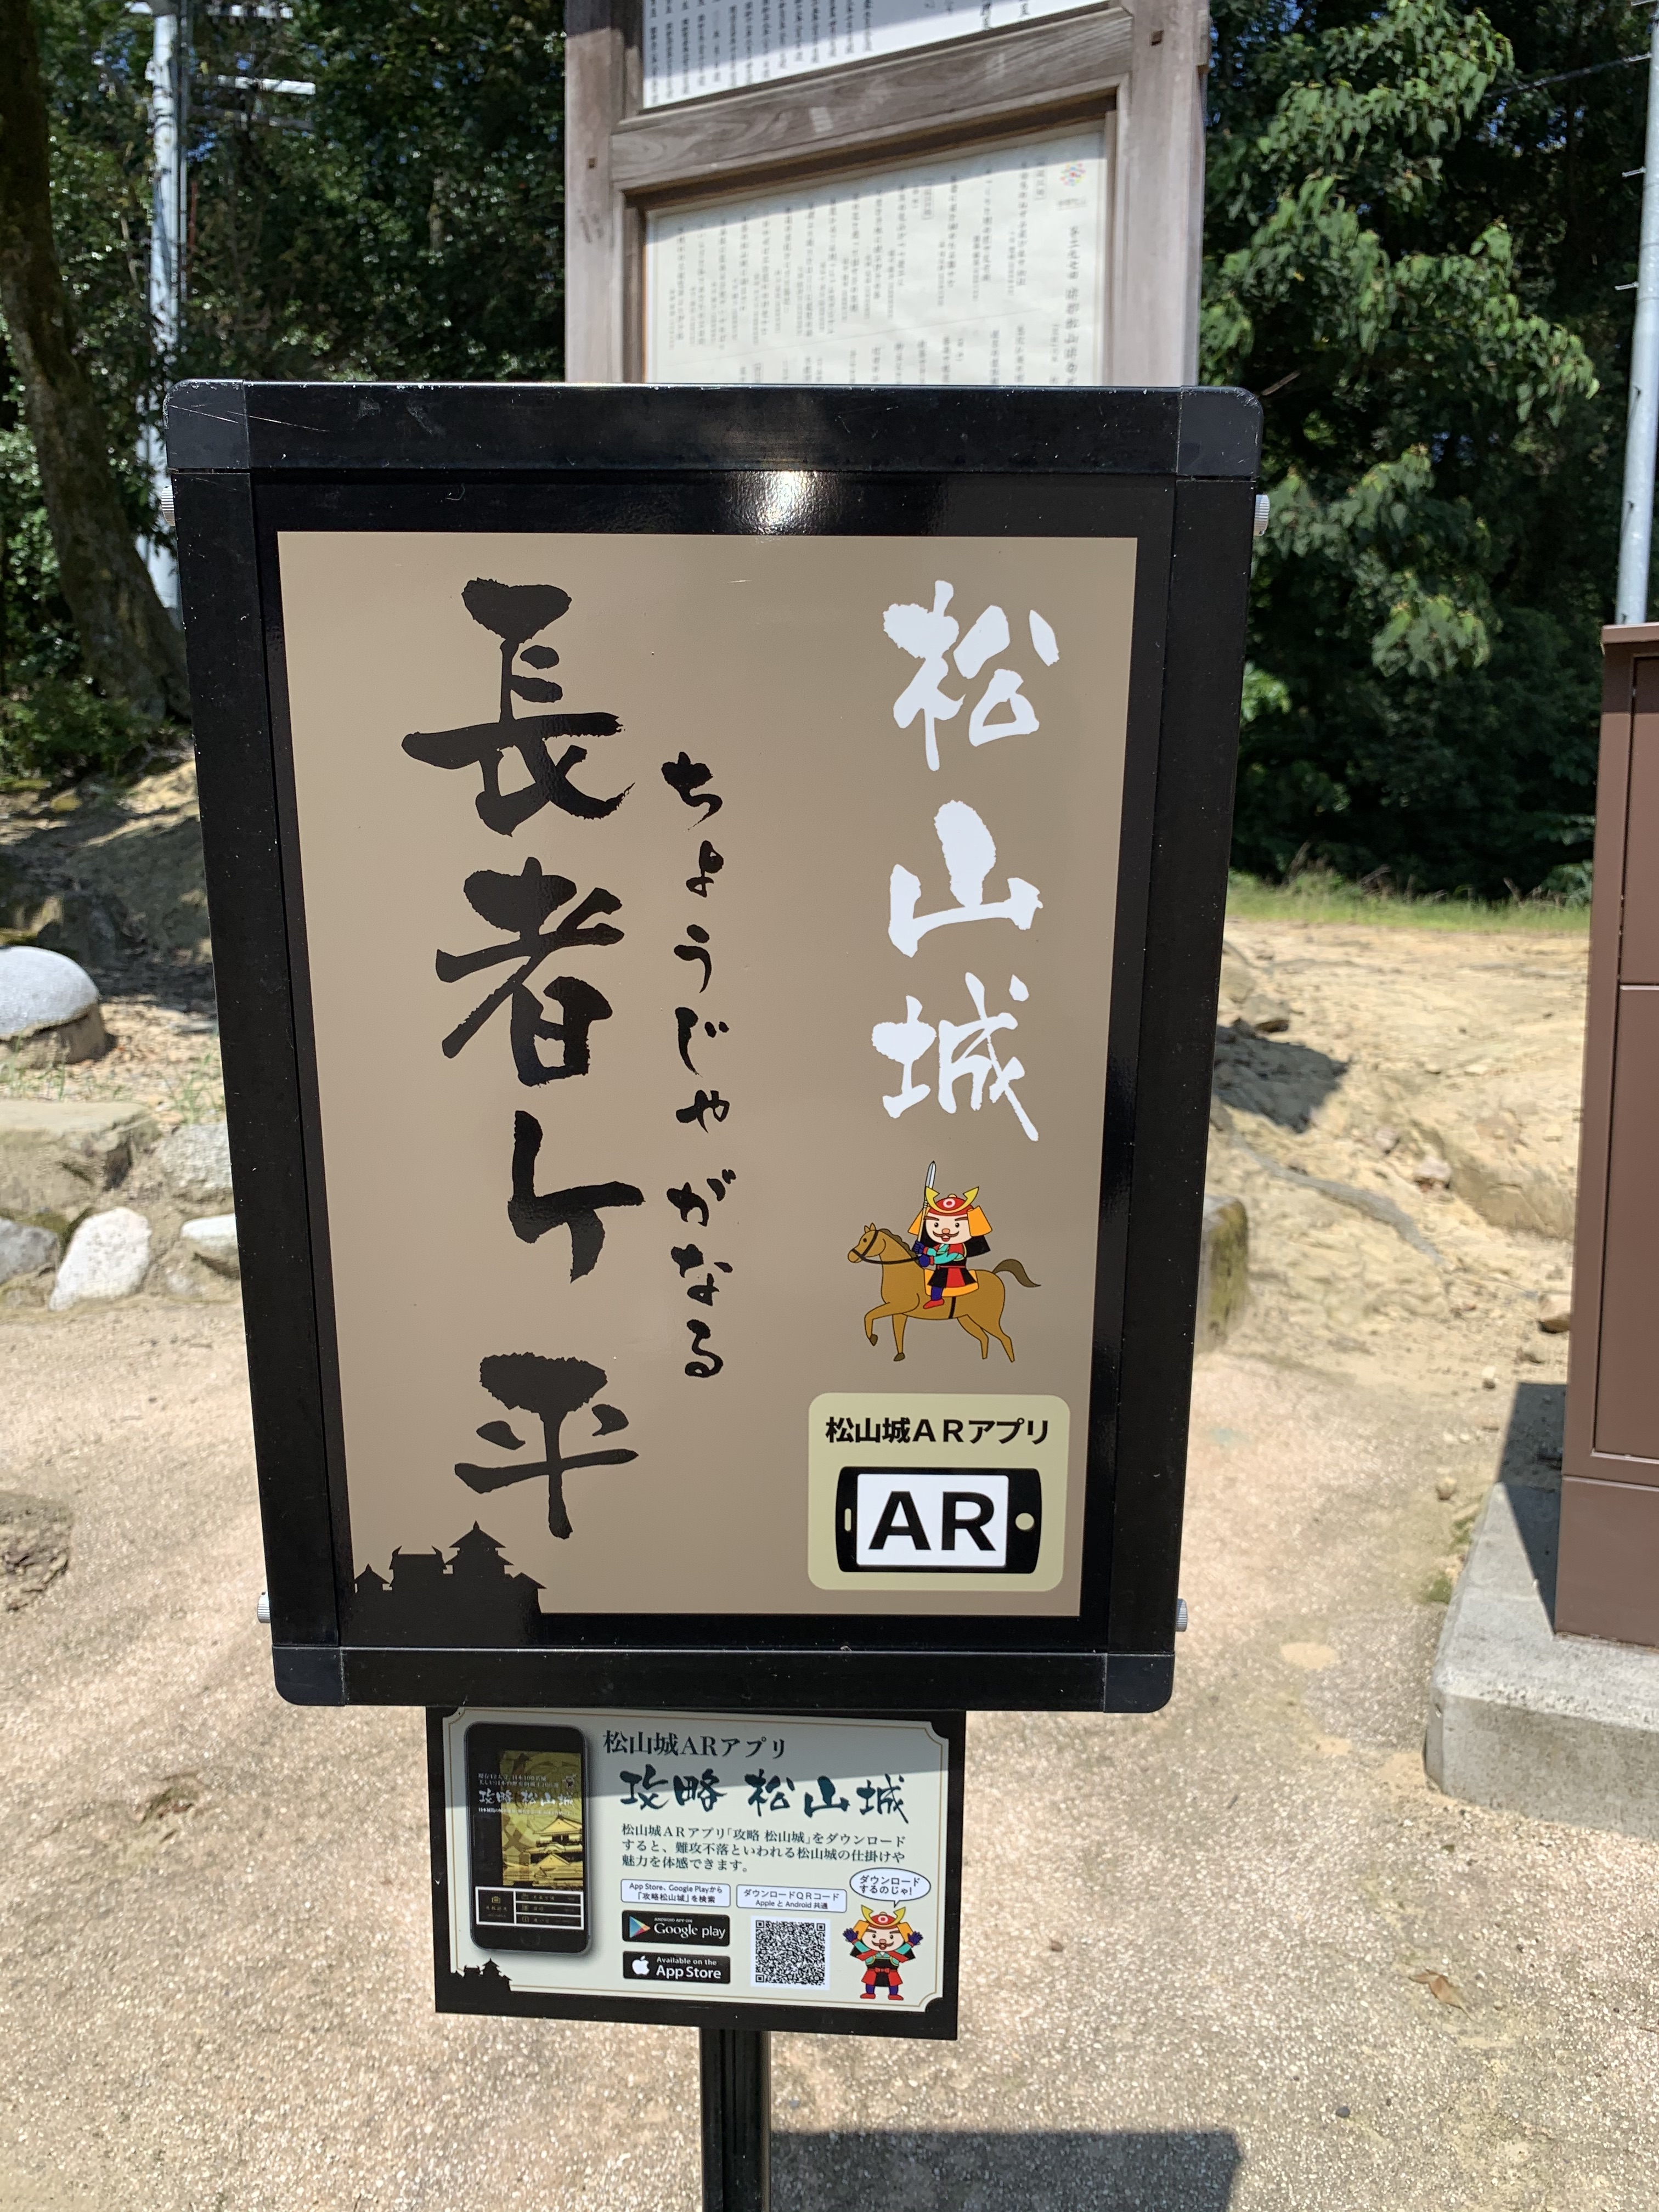
\includegraphics[width=70mm]{images/matsuyama_marker.jpg}
    \caption{専用のマーカー} \label{fig:matsuyama_marker}
  \end{minipage}
  \begin{minipage}{0.5\hsize}
    \centering
    \includegraphics[height=100mm]{images/matsuyama_ar.png}
    \caption{ARでの案内} \label{fig:matsuyama_ar}
  \end{minipage}
\end{figure}



\section{ARによるナビゲーションの問題点}
\label{problems}
前節で述べた現状を元に既存のARによるナビゲーションシステムの問題点を整理する。
ARのナビゲーションシステムには以下のような問題点がある。

\begin{itemize}
  \item 立ち上げるまでのインタラクションが面倒\\
    前節の「遺跡・史跡のARナビゲーションアプリ」のようにマーカーベースのARナビゲーションでは(1)設置されたマーカーを元にアプリを選択、(2)アプリを起動、(3)カメラでマーカーを中心に収めるという3ステップが必要になる。
    GPSと方位情報から位置測位を行うアプリケーションの場合、このような手順は必要ないが後述するように精度が悪く用途か限られるという問題がある。
  \item 位置測位の方法によって精度や用途が大きく限られる\\
    ARでのナビゲーションを行う際に多く用いられる位置測位の方法は、(1)マーカーを使う方法と(2)GPSによる座標検知と方位情報をあわせて利用する方法の2通りに大別される。
    (1)の場合マーカーが読み込めれば精度は高いが、ある程度の距離からカメラで十分認識できるサイズのマーカーを設置する必要がある。
    (2)の場合特別な設備は必要ないが精度面に疑問が残ることに加え、GPS電波の届く屋外に利用が限定される。
    前節で挙げたGoogleMapのAR機能ではGPSや方位情報に加えGoogleが撮影した道路の画像を元に補正を行い、精度を上げているが周囲の景色が登録されていない屋内での利用ができないという問題点は残る。
  \item 情報の登録・編集が面倒\\
    ARで単に目的地の位置を表示したり、決め打ったデータを表示するARナビゲーションアプリは多いが、情報の登録や編集の簡易さに焦点を置いた物は少ない。
    一方でARで表示したい情報は常に変化する可能性があり、今後も増加していくことが予想される。
    このような状況で一般ユーザが気軽に情報を登録編集できる環境を整えることは非常に重要である。
  \item 関連情報を参照・管理することができていない\\
    ARでの表示する情報が増えるにしたがってそれらを互いに参照したり、ドメインごとに管理するニーズは高まっていく。
    しかしながら既存のナビゲーションアプリではARで表示した情報同士を互いに参照して関連情報を表示したり、特定の分野でや条件でフィルターすることが難しい。
  \item 汎用性のあるアプリケーションがない\\
    上記のように「情報の登録・編集が面倒」、「関連情報を参照・管理することができていない」という問題点から特定の目的や分野に限ったARナビゲーションアプリは存在するものの、分野や目的を横断した汎用的ARナビゲーションアプリは開発されていない。
    そのため現状では目的や施設ごとにアプリケーションをユーザ側で切り替える必要があり、ARナビゲーションアプリが増えるほどユーザの負担は大きくなる。
    ユーザの目的やニーズは多岐に渡るためニーズごとにアプリケーションを分けて推薦するのではなく、様々な種類の情報を包括的に管理できるシステムが求められている。
    さらに目的や施設ごとにアプリケーションと情報が独立してしまうことで分野を横断したつながりを表現できないという問題点も生まれる。
\end{itemize}



\section{テキストや画像の進化}
前節で述べたとおりARによるナビゲーションには課題が多いが、ナビゲーションに利用しているテキストや画像などのメディアは計算機の進化とともに発展し、多くの問題点を克服している。

計算機上で利用されているテキストは、文字から内容を検索することが可能なため文書の参照や管理が格段に行いやすく、あらゆる文書が電子化されたテキストに置き換えられるようになった。
またWebやハイパーリンク等の技術によってより参照しやすくなったほか、別の文書を引用する等の再利用が可能になった。
さらにハイパーリンクを含んだ文書を手軽に作成・編集できるWiki\cite{Leuf2001TheWW}が登場したことでより柔軟で活発なテキストによる知見の共有や情報の再利用が実現された。

同様に画像や地図などのメディアも電子化とWebの進歩により参照や管理が格段に行いやすくなった。
SNSや画像の管理が行えるクラウドウェアの普及により誰しもが写真を撮影し容易にWeb上にアップロード/公開することが可能になった。
このようにして公開された画像はURLによって一意に参照することができ、画像の再利用性は大きく高まった。
またGoogle Mapsのように、地理情報システム(GIS : Geographic Information System)が誰でも検索・参照可能な形でWebに公開されることで位置情報や地理情報を参照することが容易になった。

このような文書以外のメディアの進化に合わせ、近年の文書作成システムやWikiシステムは画像/音声/動画/地図といったマルチメディアを自在に埋め込む機能を持っている。

\section{Wikiとナビゲーションへの利用}
\subsection{Wiki}
WikiはWard Cunninghamが提案した不特定多数のユーザーが文書コンテンツを編集・管理するためのWebシステムである。
Wikiには以下のような特徴があり、情報を集積するコンテンツで多く活用される。
\begin{itemize}
  \item ブラウザを使って誰でもWeb上で情報編集/共有ができる、
  \item 文書間にリンクが張りやすく、個々の文書が高度に連携した文書群を作成しやすい
\end{itemize}

\subsection{現状のナビゲーションの限界}
第\ref{current}節で挙げたとおり現状のナビゲーションシステムは決まった目的地へ案内することを目的とする物が多い。
また目的地の検索機能を有していても、ユーザは能動的にキーワードを入力し目的地を絞り込む必要がある。
一方で、ナビゲーションを必要としているユーザの多くは漠然と達成したいことがあっても実際の目的地が分かっていない。
場合によっては達成したいこと自体が曖昧で言語化できていないこともある。
このような場合、ユーザに目的地を指定・検索させて案内をする現状のナビゲーションではユーザの目的を達成する事ができない。
ユーザ側に目的に関する知識や明確な意思がない場合に案内をできないことが現状のナビゲーションの限界であると言える。

\subsection{Wikiの有用性}
上記のようなナビゲーションの限界を解決するために必要な要素は以下であると考える。
\begin{enumerate}
  \item 幅広い分野の情報を提示することができる
  \item ユーザが周囲の情報を能動的に探索できる
  \item その結果自身の目的を明確化し目的地を確定できる。
\end{enumerate}
このような要素は情報管理ツールとしてWikiを利用すること満たすことができる。
Wikiは情報を分野で階層化・グルーピングすることなく一元的に管理する。
そのため1のように分野にとらわれない情報の提示が可能である。
またWikiはハイパーリンクによって文書間で参照しており、関連情報へのアクセスが容易である。
この特徴によって2のようにリンクをたどりながら自分の興味のある分野へページを遷移し、情報を探索することができる。
さらに探索によってユーザは周囲の情報を知識として吸収し、3のように目的を明確化することができる。
以上のような理由からナビゲーションにWikiを利用することで既存のナビゲーションの限界を打破した新しい形のナビゲーションが提供できると考える。


\section{NFC技術とインタラクション}
ARでのナビゲーションシステムには自身の位置情報やその場のコンテキスト情報が不可欠であり、一般的にそのような情報を瞬時に取得することは難しい。
一方NFCタグには以下のような特徴があり、実世界においてその場のコンテキスト情報や設置された物の情報を記述するのに便利である。

\begin{itemize}
  \item 電源がいらない
  \item 非常に薄く、小型
  \item IDやURLなどを記録するには十分な記憶容量を持つ
  \item 一枚あたり10円前後と安価
\end{itemize}

近年では多くのモバイル端末にNFCタグの読み取り機能が搭載されており、一般的なNFCタグであれば誰でも書き込まれた情報を瞬時に読み取ることができる。
さらに書き込むデータ形式によっては、モバイル端末でNFCタグの読み取るだけでWebページを開いたり、アプリを起動することが可能である。

このようなNFCタグの特徴は、現在一般的な用途である決済や在庫管理、家電操作などに加えナビゲーションシステムを補助するシステムとして有効であると考える。

一方でNFCタグは読み取る際に、読み取る機器をNFCタグにかなり近づける必要があるという制約がある。
この技術的制約は一般的にデメリットとして捉えられがちであるが、NFCタグを読み取ったタイミングでのユーザの持つ端末の位置はNFCタグとほぼ接していると確定できるとも言える。
つまりNFCタグに位置情報をもたせることができれば非常に小さい誤差でユーザの持つ端末をの位置を確定できることになる。
この特徴は第\ref{problems}節で述べた問題点の1つであるNFCの位置測位の問題を解決する。





\section{まとめ}
ARをナビゲーションとして利用するアイデアは以前から存在し、モバイル端末の普及と発展により実用段階に来ているプロダクトも増えている。
しかしながら第\ref{problems}節に上げた問題点を解決できていないため、汎用的なヘルプ・ナビゲーションとして利用されるに至っていない。
一方でナビゲーションに利用しているテキストや画像などのメディアは計算機上で積極的に応用されており、ハイパーリンクやWiki等の技術によって参照や再利用がより行いやすくなった。
また近年多くのモバイル端末に搭載されているNFC技術には第\ref{problems}節であげた問題点の一部を克服する可能性がある。
したがってARの正確な位置測位とコンテキスト情報の取得にNFCの技術を利用しつつ、ARで表示する情報の管理にWikiの手法を取り入れることで第\ref{problems}節に挙げた問題を解決できると考える。
次章では第\ref{problems}節に挙げたARナビゲーションシステムが持つ問題点を解決した、次世代のARナビゲーションシステム「HypAR Touch」を提案する。  % 本文2
\chapter{設計}
\label{chap:design}

本章では次世代のARナビゲーションシステム「HypAR Touch」の要件と設計について述べる。

\newpage

\section{要件}
前章で整理したARナビゲーションシステムの問題点を踏まえた上でHypAR Touchシステムの要件を整理する。
\begin{enumerate}
  \item 手軽なインタラクションでアプリケーションの起動と位置測位ができる。
  \item 周囲のコンテキストを簡単に指定できる。
  \item ARでの表示情報を容易に登録・編集できる。
  \item ハイパーリンクを利用し、関連情報を参照・管理することができる。
\end{enumerate}
これらの要件を満たすARナビゲーションシステムは、NFCをタッチするインタラクションとハイパーテキストの編集環境であるWikiの組み合わせによって実現できる。

\section{設計}
NFCを利用したインタラクションとWikiを採用することで前節に上げた要件を満たすことを説明し、本システムの設計を記述する。

\subsection{NFC技術の利用}
前章で述べた通りNFCタグの持つ様々な性質はナビゲーションシステムにとって有用である。
この性質を利用し、NFCタグのタッチからアプリの起動と位置測位を行うことで前節の要件1を満たすことができる。
またNFCタグに記録された情報から周囲のコンテキストを把握することで前節の要件2が達成される。

\subsubsection*{要件1:手軽なインタラクションでアプリケーションの起動と位置測位ができる}
NFCタグによるインタラクションにはカメラでマーカーを読み込むインタラクションなどと比べて以下のような優位性がある。
\begin{itemize}
  \item データの読み込みが非常に早い
  \item モバイル端末でアプリが起動していない状態でも読み込み可能である
  \item 周囲の明るさなどの環境要因に左右されず安定して読み込み可能である
\end{itemize}
このようなNFCタグによるインタラクションの特徴を利用し、HypAR Touchでは次のような動作を設計した。
\begin{enumerate}
  \item NFCタグに緯度経度・方位の情報を記録する。
  \item NFCタグへのタッチを契機にアプリケーションを起動する。
  \item NFCタグを読み取るには数センチ以内の距離で平行にタッチする必要があるため、モバイル端末の位置が確定する。
  \item 3での前提を元にNFCタグに記録された緯度経度・方位の情報から初期位置を算出する。
  \item アプリの起動後は4で設定した初期位置とモバイル端末の加速度センサによるデータを組み合わせ位置を算出する.
\end{enumerate}
これにより「NFCタグにタッチする」という手軽なインタラクションでアプリケーションの起動及び位置測位が実現できたことになる。

\subsubsection*{要件2:周囲のコンテキストを簡単に指定できる}
NFCタグには上記の特徴以外にも以下のような利点がある。
\begin{itemize}
  \item 小型である
  \item 電源がいらない
  \item 情報を埋め込める十分な容量
\end{itemize}
このような特徴は実世界に設置し周囲のコンテキスト情報を記録する媒体として非常に優れている。
本研究においてはNFCタグを利用し、緯度経度情報や方位の情報のみならず設置している物や場所に合わせた情報なども記録する。
また本システムは普及に向けた観点から、事業者やユーザーなどシステムに詳しくない一般人がタグを設置するを想定している。
そのためNFCタグを利用することには上記の理由に加え以下のような点からもメリットがある。
\begin{itemize}
  \item 1枚あたりのコストが十数円と非常に安価である
  \item 読み込み距離を担保できれば外見を気にすることがなく設置が楽である
\end{itemize}
本システムではこのような特徴を活かし、誰もがNFCタグを設置できるよう一意なIDを記録したNFCタグを配布し、
貼り付けた場所の情報をアプリから登録する方法を採用した。


\subsection{Wikiの利用}
Wikiはハイパーリンクを含んだ文書を手軽に作成・編集・管理できるツールである。
WikiシステムをAR情報の管理・編集ツールとして利用することで前節の要件3、4を満たすことができる。

\subsubsection*{要件3:ハイパーリンクを利用し関連情報を参照・管理することができる}
Wikiはハイパーリンクによってページ間にリンクを張ることができ、個々のページが高度に連携した文書群を作成することができる。
その結果適切にリンクが貼られていれば文書内のリンクを辿るだけで容易に関連情報を参照することが可能である。
このようなWikiの特徴はナビゲーションシステムにおける関連情報の提示に適しているといえる。

\subsubsection*{要件4:ARでの表示情報を容易に登録・編集できる}
現在多く使われるWikiシステムにはWeb上で内容を編集する仕組みが標準で備わっており、誰もが容易に内容を登録・編集することが可能である。
またハイパーリンクやタグの記述に加え、画像や動画といったメディアの参照・埋め込み機能に対応しているシステムも多い。
このように高機能な編集機能をもったWikiをARナビゲーションの情報源として利用することでAR情報を容易に登録・編集できる環境を実現する。

\begin{figure}[H]
  \centering
  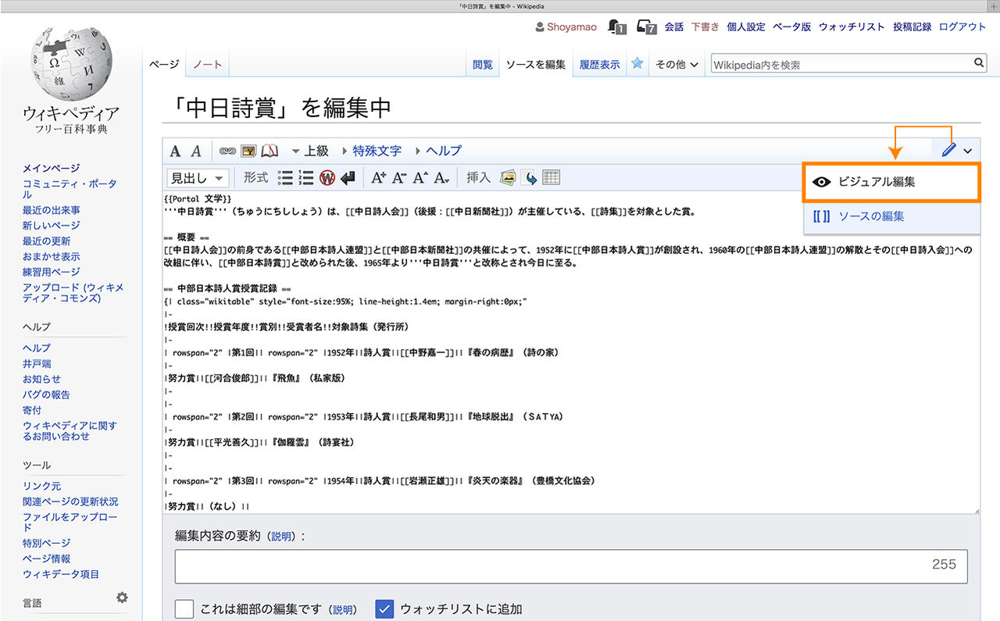
\includegraphics[width=120mm]{images/wikipedia_edit.png}
  \caption{Wikipediaでの編集画面} \label{fig:wikipedia_edit}
\end{figure}

\subsection{NFC技術とWikiの併用}
上記のようなNFC技術とWikiの利点を組み合わせることで前節の要件5も満たすことができる。

\subsubsection*{要件5:広い分野の知見と用途を総合的に管理できる}
Wikiはハイパーリンクで情報を整理・参照するため、グループによる情報分類や階層的な情報の管理を必要としない。
したがってWikiでは異なる分野の情報をフラットに管理し、参照することができる。
実際ににWikiシステムを利用した百科事典であるWikipediaはあらゆる分野の情報を総合的に管理しながらも破綻なくシステムを運用している。
このようなWikiシステムをAR情報の管理に利用することで、分野を横断した知見の管理が可能になり、様々な用途に対応したナビゲーションシステムを作成できる。

Wikiシステムを利用すると広い分野の情報を一元的に管理することができるが、一方で自身の欲しい情報を探す際に手間となる事がある。
これを避けるためにNFCタグに記録されたコンテキスト情報を活用し検索・フィルタが可能なシステムを本研究では採用した。

これより広い分野の情報を一元的に管理できるWikiの利点を活かしながら様々な用途に対応したナビゲーションを提供する事が可能となる.



\section{まとめ}
本章では第\ref{chap:background}章で整理したARナビゲーションの現状と問題点を元に次世代ARナビゲーションシステム、HypAR Touchの要件を定義した。
さらに定義した要件はNFC技術とWikiシステムを組み合わせることで達成されることを提案し、その詳細を設計で示した。
次章では本設計を元に開発したHypAR Touchの実装とその機能を説明する。  % 本文3
\chapter{実装}
\label{chap:implementation}

本章では第\ref{chap:design}章で述べたシステムの設計を元にした、HypAR Touchの実装及び機能について述べる。

\newpage

\section{アプリケーション構成}
HypAR TouchはARナビゲーションを表示するモバイルアプリケーション、AR情報やNFC情報を永続化しAPIを提供するサーバー、Scrapbox、Gyazo\footnote{\textsf{https://gyazo.com}}、NFCタグで構成される(図 \ref{fig:application_structure})。

\begin{figure}[H]
  \centering
  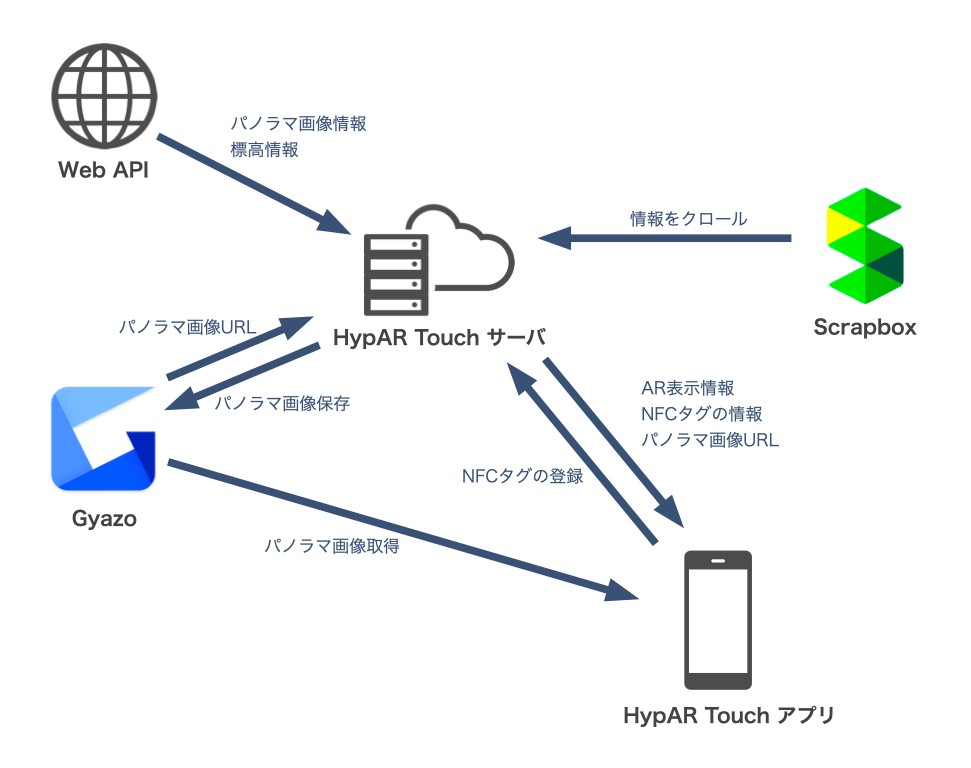
\includegraphics[width=150mm]{images/application_structure.jpg}
  \caption{構成図} \label{fig:application_structure}
\end{figure}

\subsection{Scrapbox}
Scrapbox(図\ref{fig:scrapbox})はGyazz\cite{Gyazz}をベースにして開発された、Nota\footnote{\textsf{https://www.notainc.com/ja}}社が運営しているWikiである。
本システムではこのScrapboxをARで表示する情報の管理ツールとして利用している。
これはScrapboxが他のシステムには存在しない以下のようなHypAR Touchに適した特徴を持つためである。
\begin{itemize}
  \item シンプルで柔軟な記法をもつWYSIWYGエディタ
  
  入力/改行/段落/箇条書きといった基本的なテキスト編集を見たまま行える。
  
  \item 場所指定に最適なLocation記法
  
  Google MapsのURLを貼り付けるだけで地図を埋め込めるLocation記法\footnote{\textsf{https://scrapbox.io/help-jp/Location記法}}と呼ばれる機能があり地理情報を記述するのに適している。
  本システムではこのLocation記法によって表示する情報の場所を指定している。

  \item リンク記法によるシンプルなハイパーリンクと関連ページリスト
  
  Scrapboxでは単語を\texttt{[]}で囲うだけで同一Wiki内ページへのリンクとすることが可能である。
  さらにScrapboxページの下部には
  \begin{itemize}
      \item 別ページへのリンク
      \item 別ページからのリンク
      \item リンク先ページがリンクしているページ
  \end{itemize}
  といった関連ページリスト(図\ref{fig:scrapbox_related})が表示され、どのような情報と関連するのかが一目瞭然に分かる。
\end{itemize}

\begin{figure}[H]
  \begin{minipage}{0.5\hsize}
    \centering
    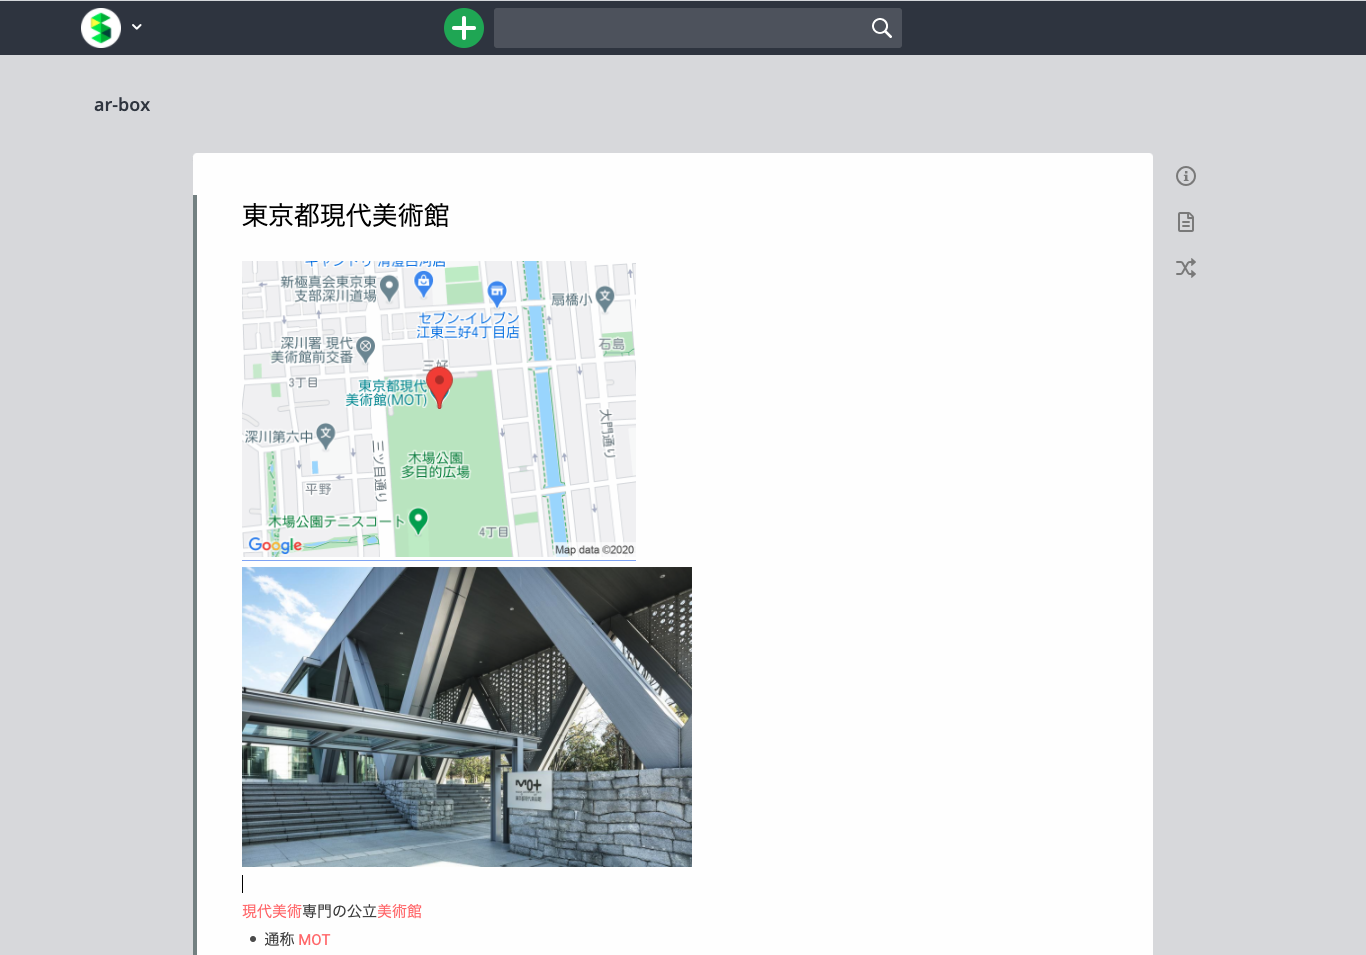
\includegraphics[width=75mm]{images/scrapbox_screen.png}
    \caption{Scrapboxの画面} \label{fig:scrapbox}
  \end{minipage}
  \begin{minipage}{0.5\hsize}
    \centering
    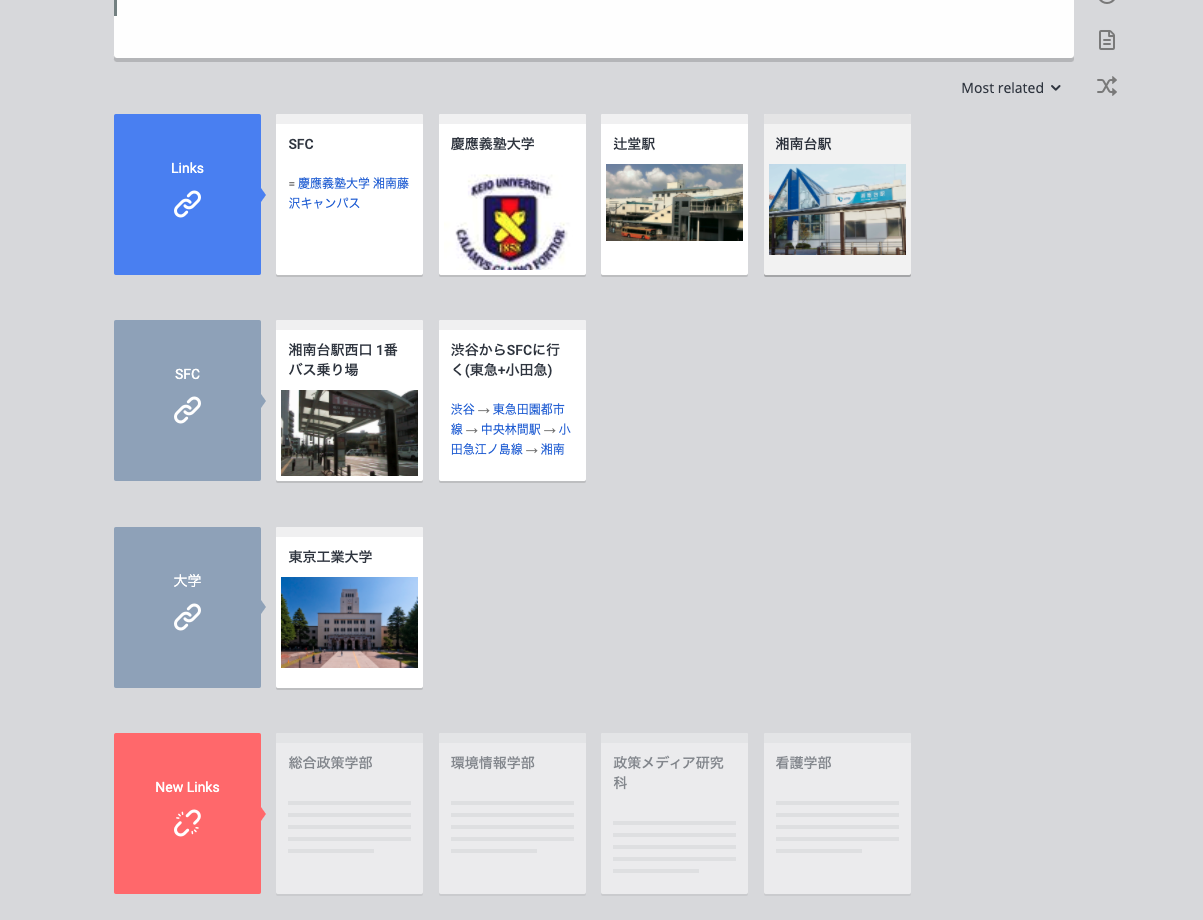
\includegraphics[width=75mm]{images/scrapbox_related_screen.png}
    \caption{Scrapboxの関連ページリスト} \label{fig:scrapbox_related}
  \end{minipage}
\end{figure}

Scrapboxでは文書の集合であるWikiを「プロジェクト」という単位で管理しており、プロジェクトによってメンバ・公開設定等を設定可能である。
プロジェクト内のページはすべてフラットに管理され、上記の記法でページ間をハイパーリンクでつなぎ容易に参照できる。
HypAR TouchではNFCタグで対象とするScrapboxのプロジェクトを選択できるようにしている。
またHypAR Touchではプロジェクト内の1ページがARで表示される1つのノード対応するようなっている。

Scrapboxはプロジェクト内のページリストと各ページの情報を取得するAPI\footnote{\textsf{https://scrapbox.io/help-jp/API}}を持っており、これを利用することでHypAR TouchサーバはScrapboxをクロールしている。


\subsection{HypAR Touchアプリ}
HypAR TouchアプリはReactNative\footnote{\textsf{https://reactnative.dev/}}と呼ばれるフレームワークを利用して作成されたモバイル端末アプリケーションである。
ReactNativeはWeb技術を利用し、マルチプラットフォームなモバイル端末向けアプリケーションを作成するためのフレームワークである。
このReactNative利用することでHypAR TouchアプリはAndroidとiOSの両方に対応したアプリケーションとなっている。

HypAr TouchアプリはNFCに記録された一意なidを取得し、そのidに紐付いた以下の情報を後述するHypAr Touchサーバーから取得する。
\begin{itemize}
  \item NFCタグの緯度経度
  \item NFCタグの設置される向き(0〜360度)
  \item 表示するAR情報の元となるScrapboxのプロジェクト名
  \item タッチした時に選択されているリンク情報
\end{itemize}
さらに取得したScrapboxのプロジェクト名をもとにHypAR TouchサーバーからARで表示する情報を取得する。
その上で取得したARの情報とNFCタグの緯度経度、NFCタグの設置された向きをもとに、各AR情報の位置を相対的に算出している。
また各AR情報には登録された位置付近で撮影されたパノラマ画像のURLが含まれている。
視点移動機能ではこのURLで登録された360度画像からVRのビューを作成している。

\subsection{HypAR Touchサーバ}
HypAR TouchサーバはNode.js\footnote{\textsf{https://nodejs.org/}}上で動作するWebアプリケーションとして実装されている。
HTTPリクエストを処理するWebアプリケーションフレームワークとしてExpress\footnote{\textsf{https://expressjs.com/}}を用い、
そのホスティング環境としてBaaS(Backend-as-a-Service)の1つであるHeroku\footnote{\textsf{https://www.heroku.com/}}を利用している。
HypAR TouchサーバはHypAR Touchアプリで利用するAR情報やNFCタグ情報を管理する役割をもっており、その機能は大きく4つに分けられる。

\begin{itemize}
  \item 対象となるScrapboxのプロジェクトをクロールし、AR表示に必要な情報を整理した上で永続化する。\\
  HypAR Touchサーバは指定されたScrapboxのプロジェクトを定期的にクロールし、位置情報やサムネイル画像のURL、リンク情報など、AR表示に必要な情報をまとめてデータベースに永続化している。
  これによりユーザがScrapboxに加えた変更がARでの表示に対応するようになっている。
  \\
  \item 登録されたNFCタグに関する情報を永続化する。\\
  NFCタグには一意なidが記録されており、それに紐づく形でタグの位置情報や向き、対象とするScrapboxプロジェクトなどの情報がこのサーバーに記録される。
  \\
  \item クロールした情報を元にパノラマ画像を生成し、Gyazoに保存した上でそのURLを記録する。\\
  第3章で記述した視点移動機能を実装するためにはARで表示する情報に加えて、記録された位置情報に最も近いところから撮影されたパノラマ画像が必要である。
  そのためHypAR TouchサーバではARで表示する情報ごとにGoogle Street ViewのAPI\footnote{\textsf{https://developers.google.com/maps/documentation/streetview/overview}}を利用してその地点からのパノラマ画像を生成している。
  また、画像の保存・永続化には後述するGyazoを利用しており、最終的にはGyazoに保存されたパノラマ画像のURLをARで表示する情報と合わせてデータベースに永続化している。
  \\
  \item 上記3つの情報を取得・追加・変更するAPIを提供する。\\
  HypAR Touchサーバは上記3つの情報を生成・永続化するだけでなく、HypAR TouchアプリからのAR情報取得やNFCタグの登録を受け付ける必要がある。
  そのためHypAR Touchサーバはこれらの情報を取得、追加、更新するAPIを提供している。

\end{itemize}


\subsection{Gyazo}
Gyazoは、パソコンのデスクトップ画面の一部をキャプチャしてWebにアップロードするツールおよび画像を保存する画像/映像専用のクラウドストレージサービスである。
Gyazoには十分な保存容量があり、画像のアップロード・取得等のAPIも揃っている。
そのため自身のサーバよりも安全に画像を管理可能なGyazoを本システムでのパノラマ画像の保存先として利用している。

\subsection{NFCタグ}
本システムで利用するNFCタグはモバイル端末のOSに関わらず、読み込めるタグ形式とデータフォーマットでなくてはならない。
そのため本システムではNFCタグとして最も普及しているISO/IEC 14443 TypeAに準拠したNFCタグを利用している。
また同様にNFC FORUMが策定したデータフォーマットであるNDEFを利用することでNFC機能を持つほとんどのモバイル端末に対応している。
NDEFのデータ形式には更に細かく、Text、URI、SmartPostermの3つのタイプが存在する。
このうちURIタイプで書かれたNFCタグは殆どのNFC対応スマートフォンでのバックグラウンド読み取りに対応している。
またAndroidとiOSにはディープリンクと呼ばれる特殊なURIからインストールされたアプリケーションを起動する機能が存在しており、そのURIの形式をCustom URL Schemeと呼ぶ。
Custom URL Schemeでは図\ref{fig:custom_url_scheme}のように起動するアプリの指定だけでなく、URIパラメータを利用して追加の情報を記述しアプリケーション側にその情報を渡すことが可能である。
このような特徴を踏まえ、本システムではNFCタグにCustom URL Schemeの形にしたURIをNDEFのURIタイプとして記録している。
これにより、モバイル端末でNFCタグにタッチするだけでアプリの起動及びタグIDの受け渡しが可能となる。

\begin{figure}[H]
  \centering
  
\includegraphics[width=150mm]{images/custom_url_scheme.jpg}
  \caption{Custom URL Scheme} \label{fig:custom_url_scheme}
\end{figure}




\section{機能}

\subsubsection{HypAR Touchアプリによるナビゲーション閲覧}
\paragraph*{NFCタグにタッチする}
本アプリケーションは図\ref{fig:touch_nfc}のように専用の情報が書かれたNFCタグにタッチすることで起動し、ナビゲーションを開始する。
NFCにタッチすることで端末の位置と向きが認識され、図\ref{fig:hypar_touch_init_screen}のように登録された情報をARで正しい位置に表示することができる。
また画面下部にあるスライダー(図\ref{fig:hypar_touch_slider})を動かすことでARで表示する情報の距離の範囲を指定することができる。

\begin{figure}[H]
  \centering
  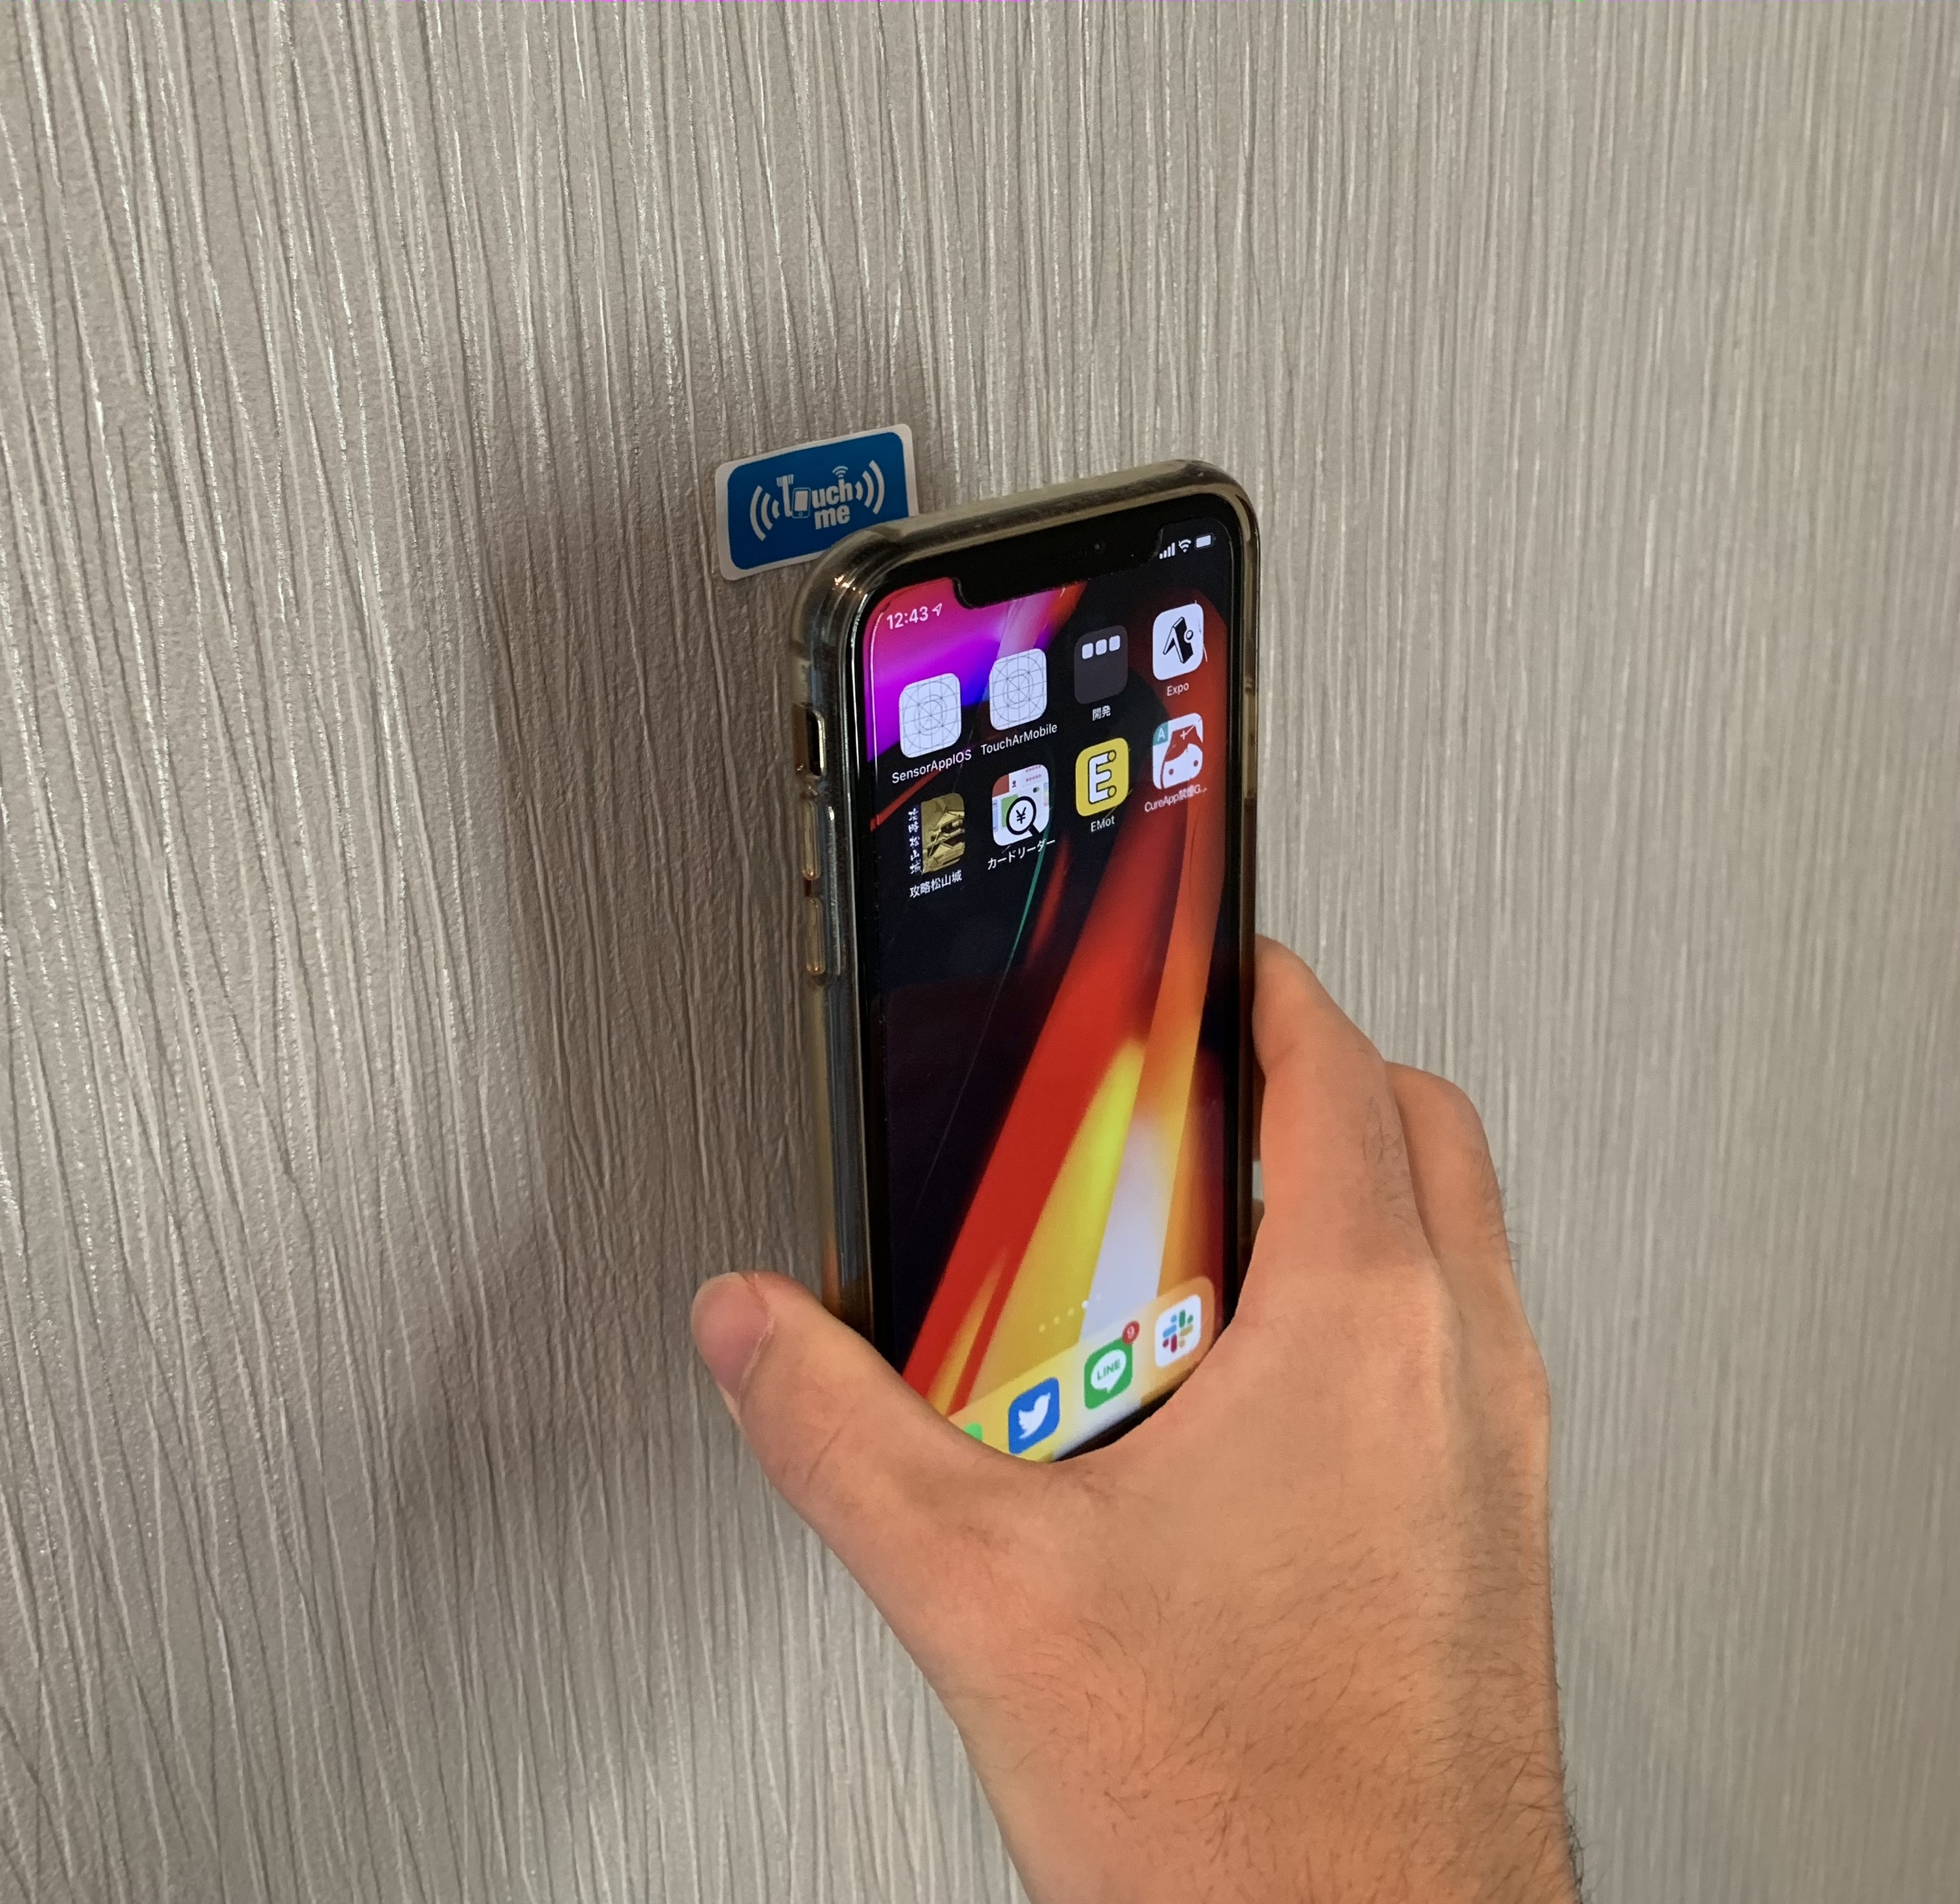
\includegraphics[width=100mm]{images/touch_nfc.jpg}
  \caption{NFCタグにタッチする様子} \label{fig:touch_nfc}
\end{figure}

\begin{figure}[H]
  \begin{minipage}{0.5\hsize}
    \centering
    \includegraphics[height=100mm]{images/hypar_touch_init_screen.png}
    \caption{ARでの表示} \label{fig:hypar_touch_init_screen}
  \end{minipage}
  \begin{minipage}{0.5\hsize}
    \centering
    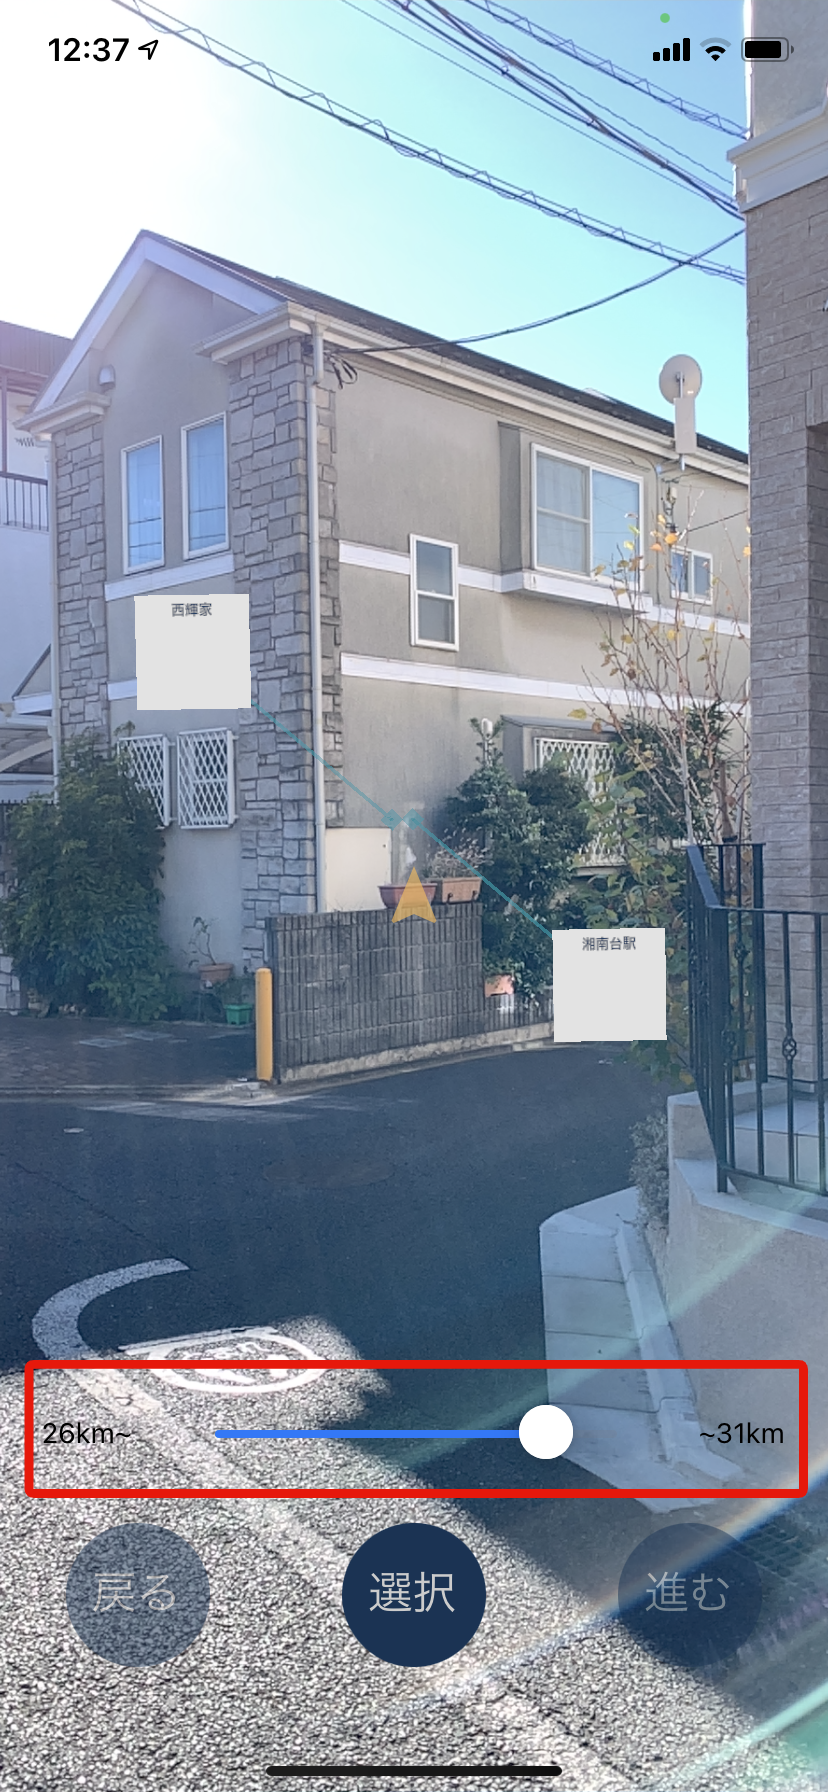
\includegraphics[height=100mm]{images/hypar_touch_slider.png}
    \caption{スライダーによる距離指定} \label{fig:hypar_touch_slider}
  \end{minipage}
\end{figure}

\paragraph*{表示されたAR情報の関連情報を表示・選択する}
画面の中央にはオレンジ色の三角のカーソルが表示されており、これをARで表示された情報の上に重ねると青い枠線が表示される(図\ref{fig:hypar_touch_hover})。
その状態で画面下部の選択ボタンを押すと図\ref{fig:hypar_touch_selected}のように関連する情報が放射状に配置されてに表示される。
これらの表示された関連情報も同じようにカーソルで選択することができる(図\ref{fig:hypar_touch_sub_selected})。
このように関連情報を選択していくことによって興味のある情報をAR上で探索することができる。

\begin{figure}[H]
  \begin{minipage}{0.5\hsize}
    \centering
    \includegraphics[height=100mm]{images/hypar_touch_hover.png}
    \caption{カーソルを重ねた状態} \label{fig:hypar_touch_hover}
  \end{minipage}
  \begin{minipage}{0.5\hsize}
    \centering
    \includegraphics[height=100mm]{images/hypar_touch_selected.png}
    \caption{選択した状態} \label{fig:hypar_touch_selected}
  \end{minipage}
\end{figure}

\begin{figure}[H]
    \centering
    \includegraphics[height=100mm]{images/hypar_touch_sub_selected.png}
    \caption{関連情報の選択} \label{fig:hypar_touch_sub_selected}
\end{figure}


\paragraph*{選択されたAR情報の詳細を見る}
上記のようにカーソルをAR情報にあわせた上で選択ボタンを押すと画面上部には図\ref{fig:hypar_touch_top}のように選択された情報のタイトルの他に「see more」と書かれたボタンが出現する。
これをクリックすることでAR情報の元となったScrapboxをみることが可能である(図\ref{fig:hypar_touch_webview})。

\begin{figure}[H]
  \begin{minipage}{0.5\hsize}
    \centering
    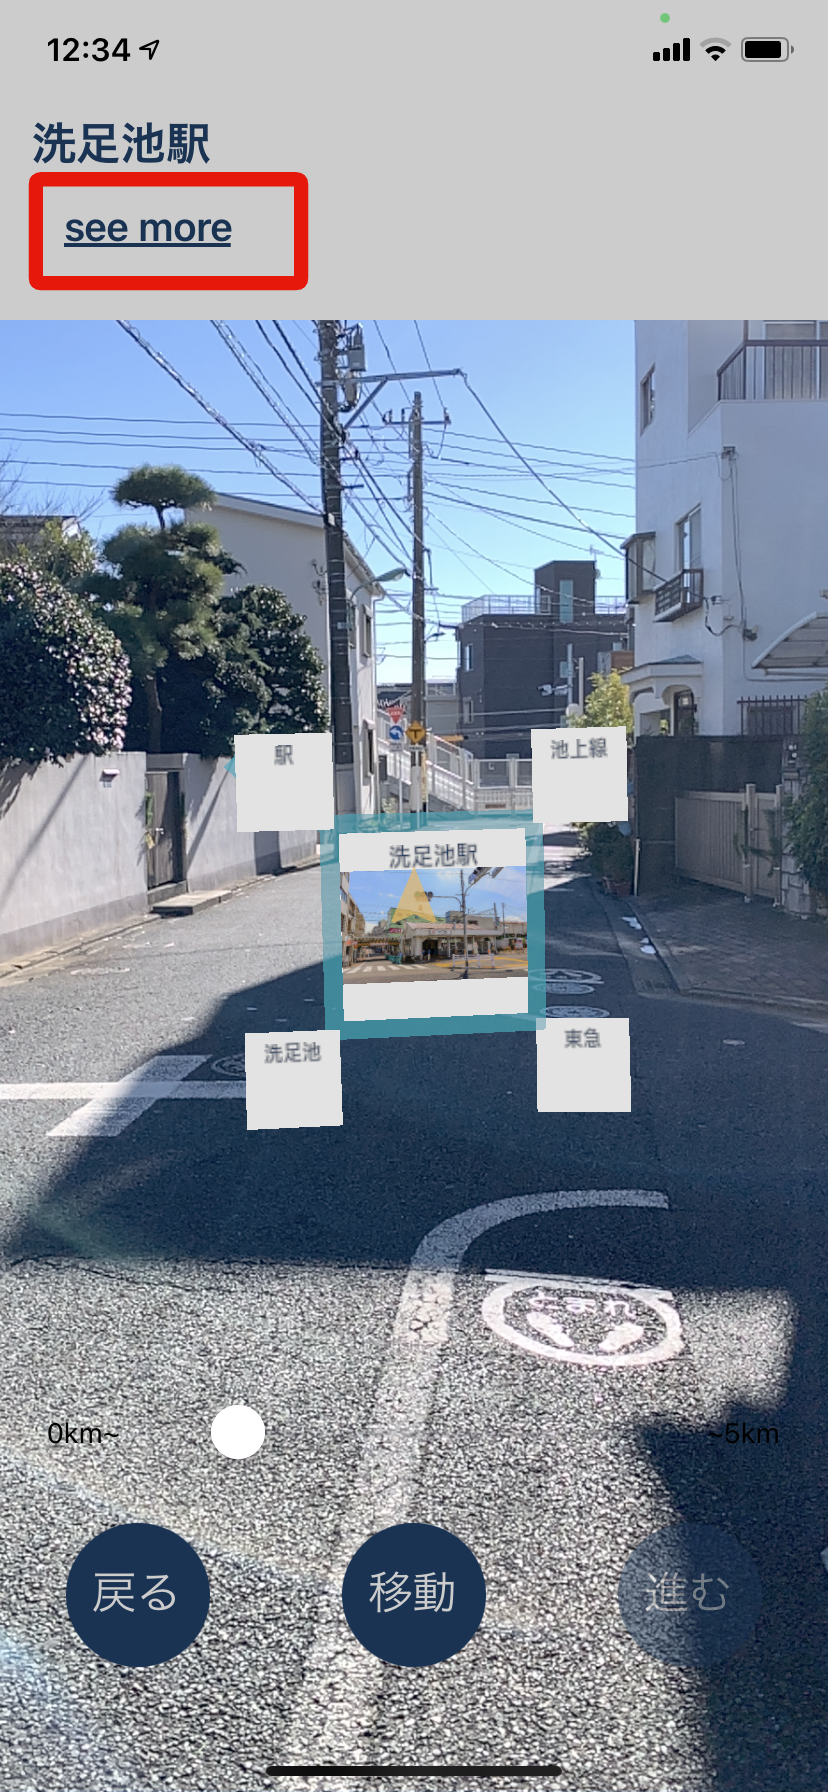
\includegraphics[height=100mm]{images/hypar_touch_top.png}
    \caption{詳細を表示するボタン} \label{fig:hypar_touch_top}
  \end{minipage}
  \begin{minipage}{0.5\hsize}
    \centering
    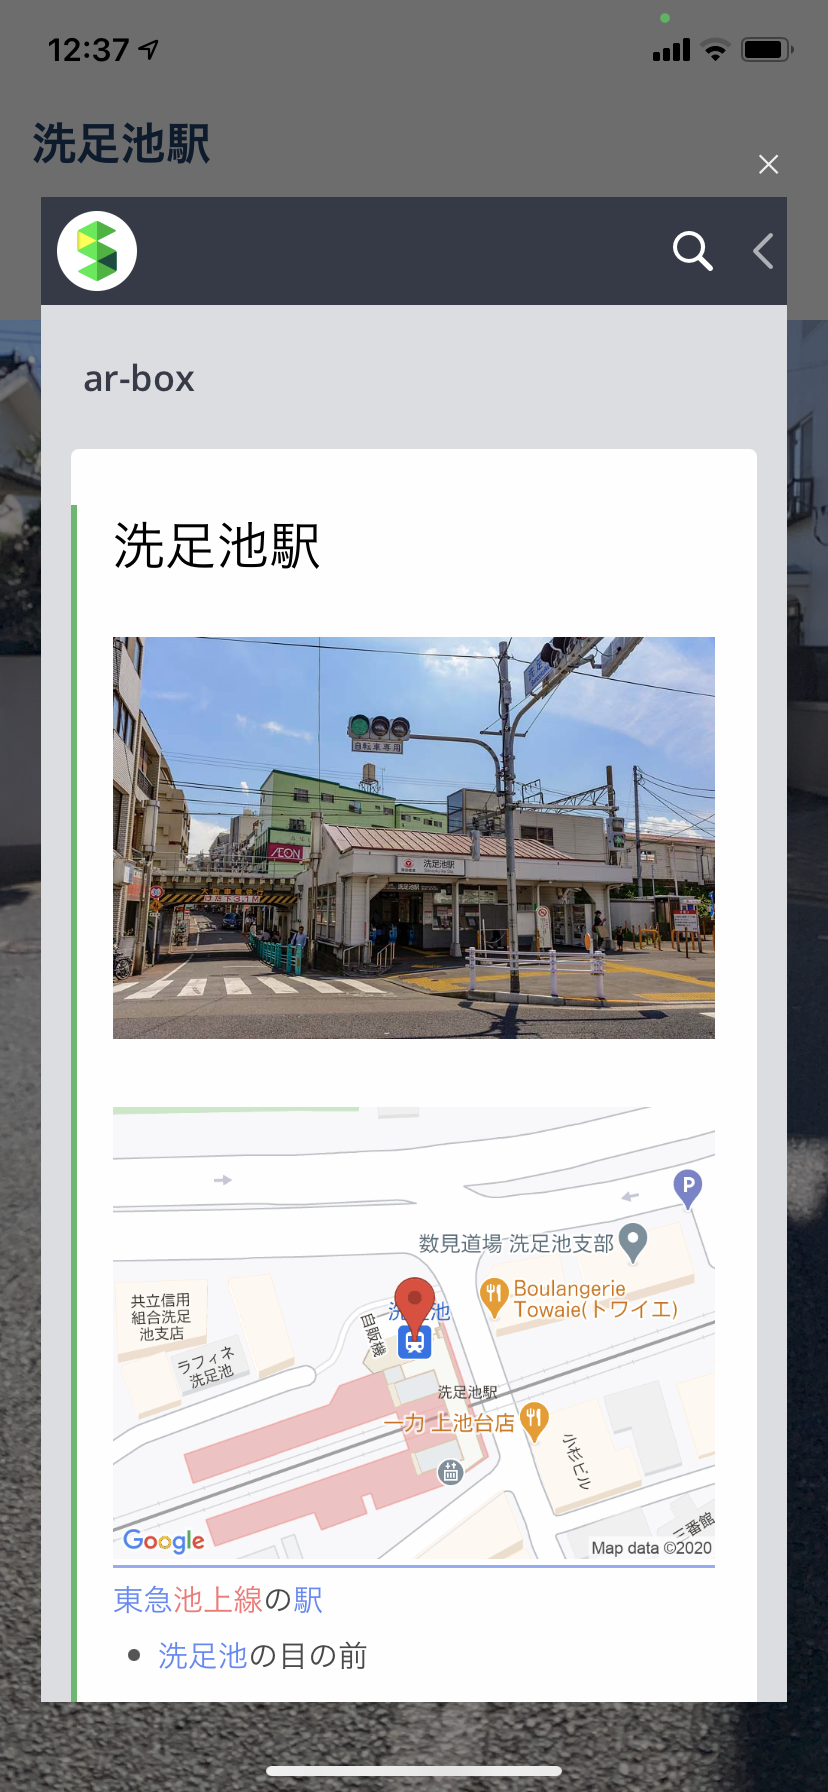
\includegraphics[height=100mm]{images/hypar_touch_webview.png}
    \caption{Scrapboxでの情報表示} \label{fig:hypar_touch_webview}
  \end{minipage}
\end{figure}

\paragraph*{選択されたAR情報の場所に視点を移動する}
同じようにカーソルをAR情報にあわせた上で選択ボタンを押し、もう一度選択したAR情報にカーソルを重ねると画面下部中央のボタンが「移動」に変化する(図\ref{fig:hypar_touch_move_button})
この移動ボタンを押すと図\ref{fig:hypar_touch_move_map}のような地図での移動アニメーションを経て、選択した情報のある場所からの視点(図\ref{fig:hypar_touch_moved})に切り替えることができる。

\begin{figure}[H]
  \begin{minipage}{0.5\hsize}
    \centering
    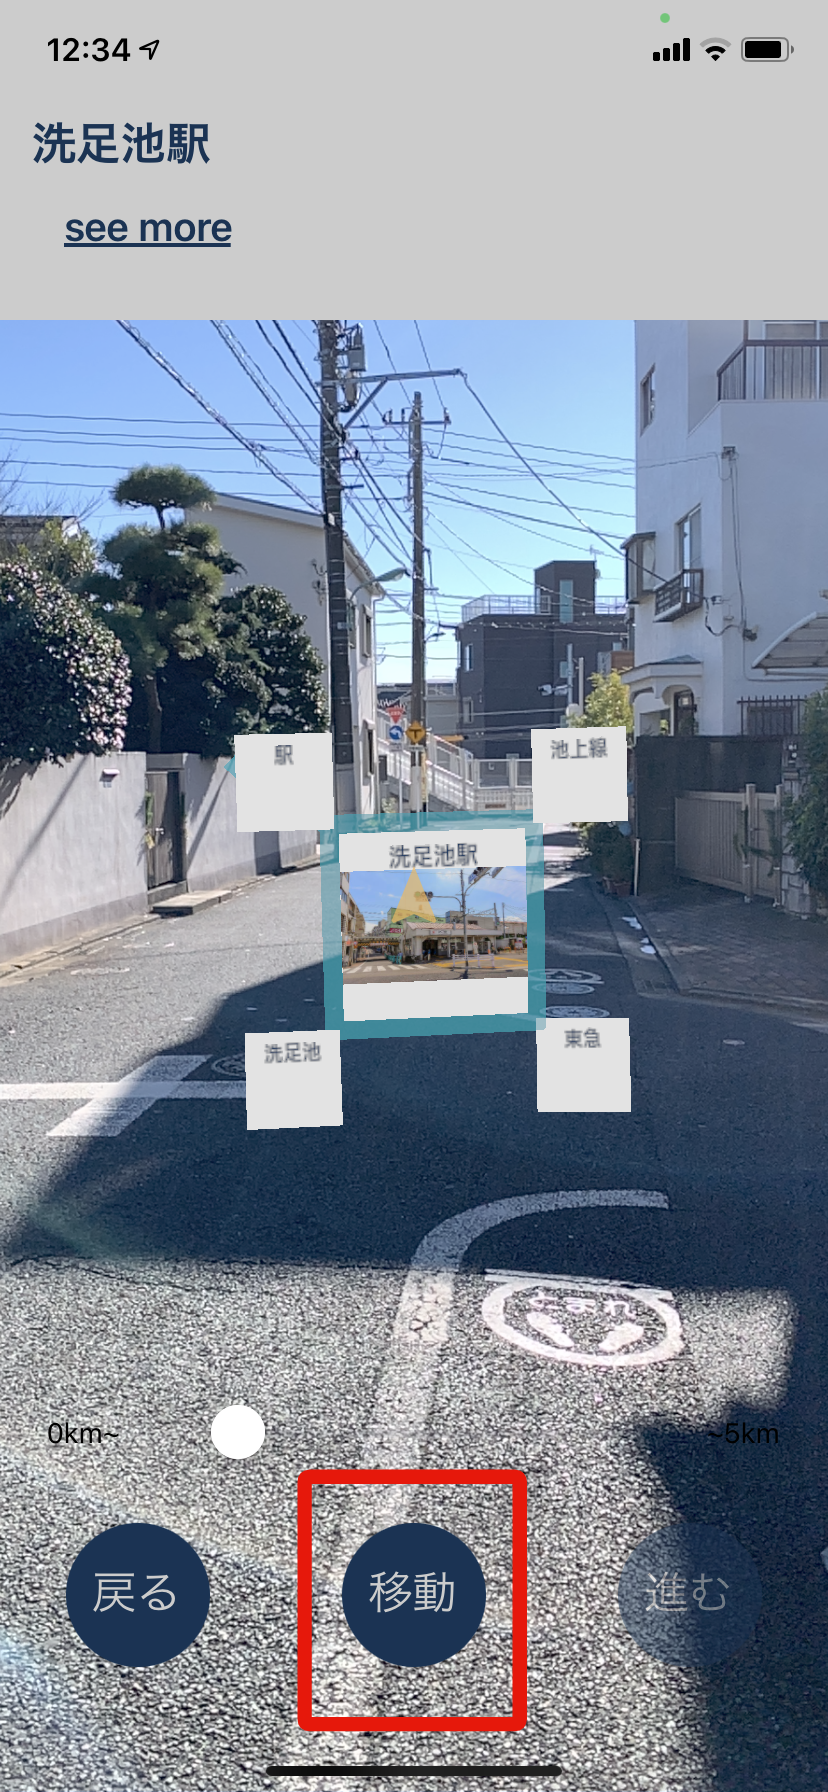
\includegraphics[height=100mm]{images/hypar_touch_move_button.png}
    \caption{移動ボタン} \label{fig:hypar_touch_move_button}
  \end{minipage}
  \begin{minipage}{0.5\hsize}
    \centering
    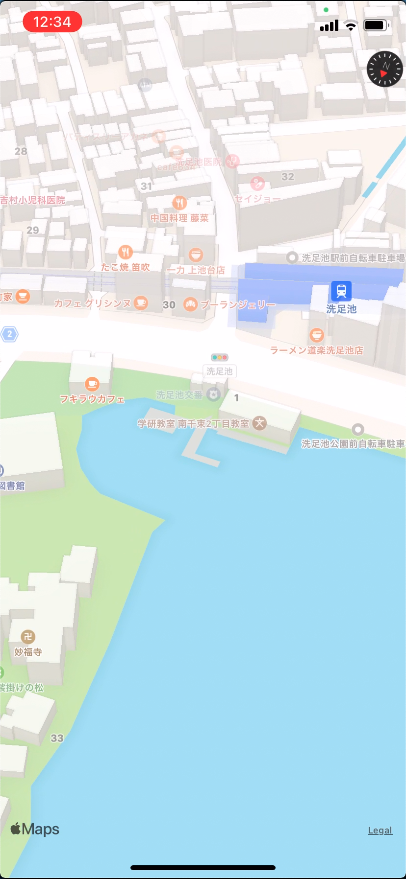
\includegraphics[height=100mm]{images/hypar_touch_move_map.png}
    \caption{Mapでの移動アニメーションの途中} \label{fig:hypar_touch_move_map}
  \end{minipage}
\end{figure}

\begin{figure}[H]
  \centering
  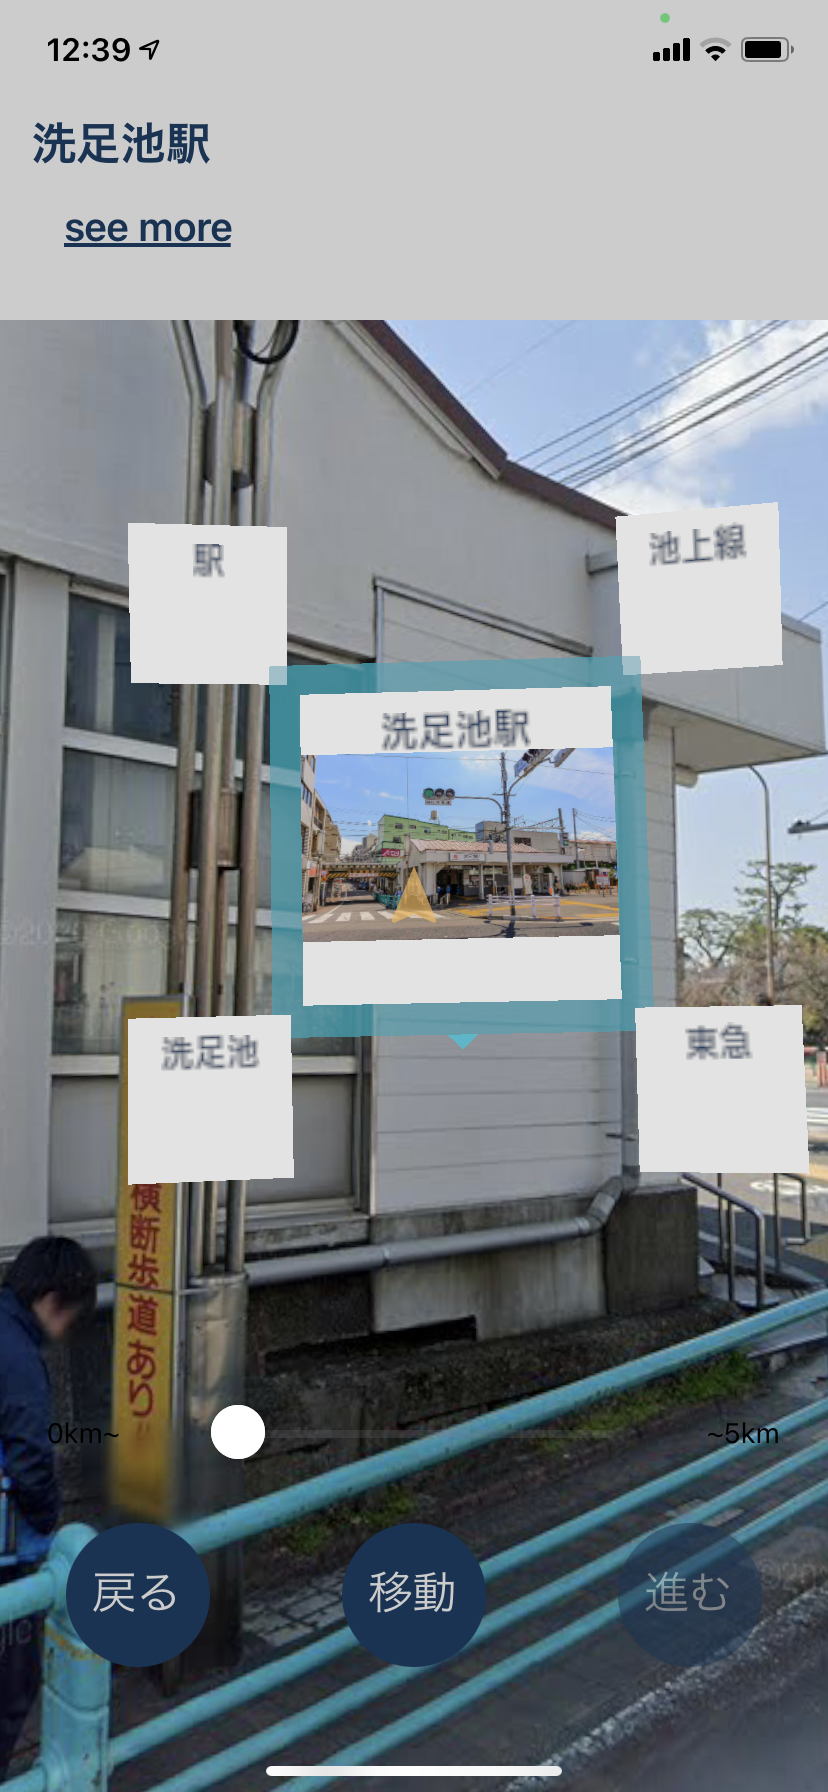
\includegraphics[height=100mm]{images/hypar_touch_moved.png}
  \caption{移動先からの視点} \label{fig:hypar_touch_moved}
\end{figure}

\paragraph*{AR情報の選択を解除する・前の状態に戻る}
上記のような選択状態は画面の何も表示されていない部分をタップすることで解除できる。
また選択や移動した履歴情報は常に保存されており、画面下部の「戻る」「進む」ボタン(図\ref{fig:hypar_touch_history_button})で履歴を参照することができる。

\begin{figure}[H]
  \centering
  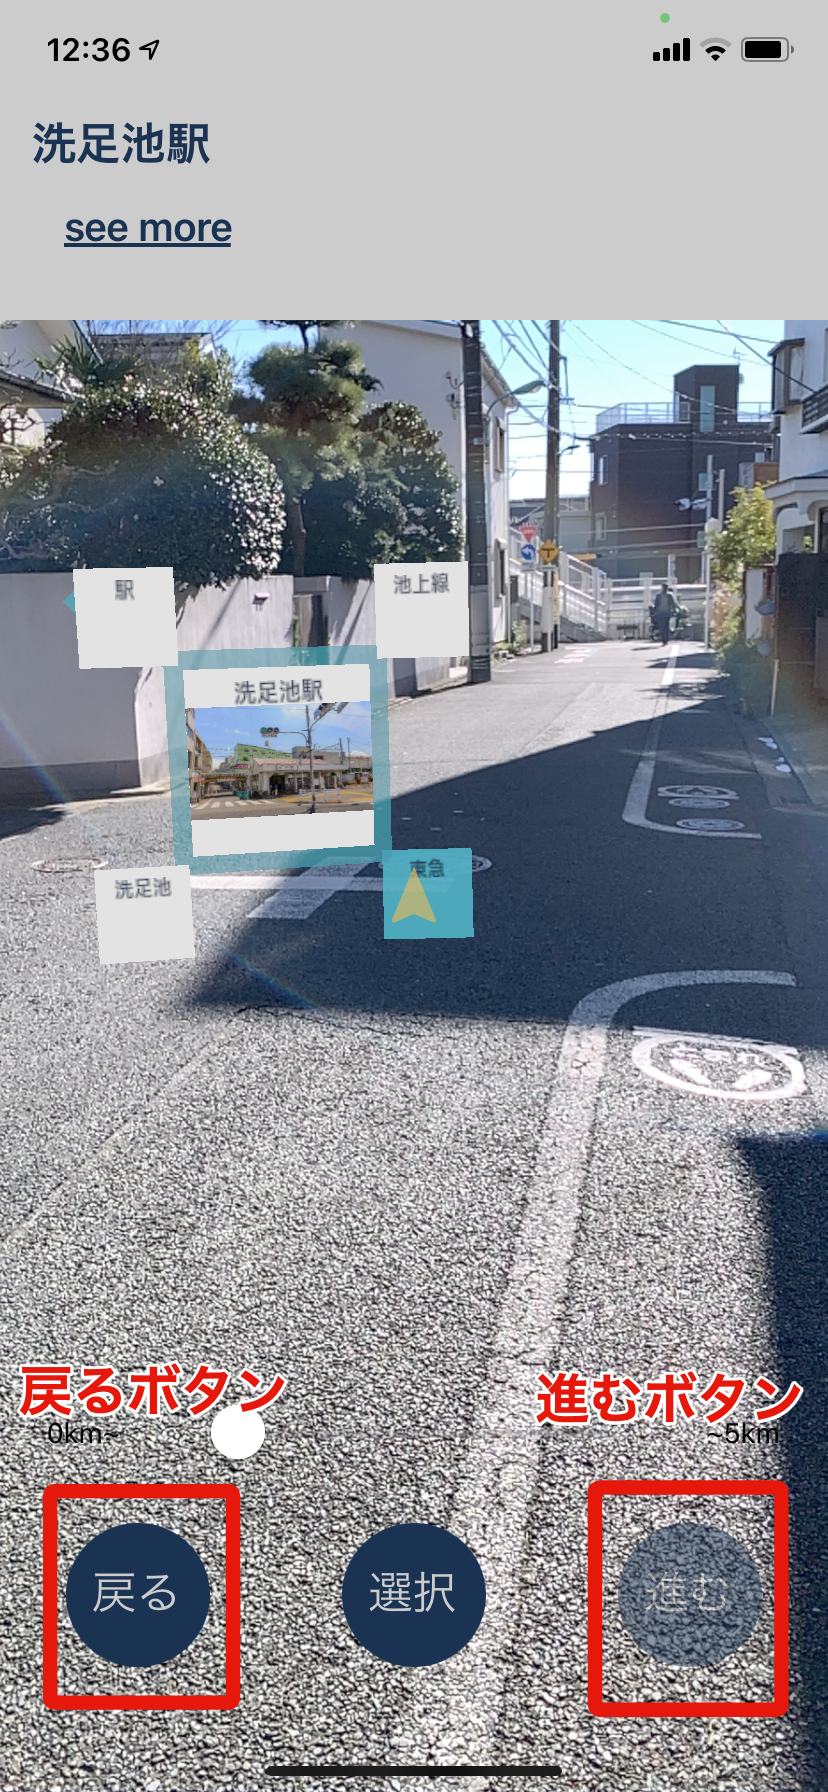
\includegraphics[height=100mm]{images/hypar_touch_history_button.png}
  \caption{進むボタンと戻るボタン} \label{fig:hypar_touch_history_button}
\end{figure}

\subsubsection{ScrapboxによるAR情報法の追加・編集}
HypAR Touchアプリに表示されるAR情報はNFCタグで指定されたScrapboxのプロジェクトをもとに生成される。
Scrapboxのプロジェクトにあるページのうち、Location記法によって位置情報の記述のあるページがアプリ側で表示されるAR情報と対応する。

\paragraph*{ARで表示する情報を追加する}
AR情報はScrapboxのページと対応しているため、新しくページを作成し、以下の2点の情報を記入することでAR情報が登録される。
\begin{itemize}
  \item ページタイトル
  
  図\ref{fig:scrapbox_ar_new}の\textcircled{\scriptsize{1}}部分であり、ページを作る上で必須となる項目である。
  このタイトルはHypAR Touchアプリ側でサムネイルとともにAR表示される。

  \item Location記法による記述
  
  Scrapboxにはソースコード \ref{google_map_url}のようなGoogle MapsのURLをソースコード \ref{location}のようなLocation記法に変換し、図\ref{fig:scrapbox_ar_new}の\textcircled{\scriptsize{2}}のようにマップとして表示する機能がある。
  この機能を利用し、AR情報を追加したい場所を中心としたGoogleMapのURLをScrapboxに貼り付けることでAR上で表示する場所を指定する。

  \begin{lstlisting}[caption=googleMapのURL, label=google_map_url]
    https://www.google.com/maps/place/%E6%9D%B1%E4%BA%AC%E9%A7%85/@35.681502,139.7671784,17z/data=!4m5!3m4!1s0x60188bfbd89f700b:0x277c49ba34ed38!8m2!3d35.6812362!4d139.7671248
  \end{lstlisting}

  \begin{lstlisting}[caption=Location記法, label=location]
    [N35.681502,E139.7671784,Z16 東京駅]
  \end{lstlisting}
\end{itemize}

\begin{figure}[H]
  \centering
  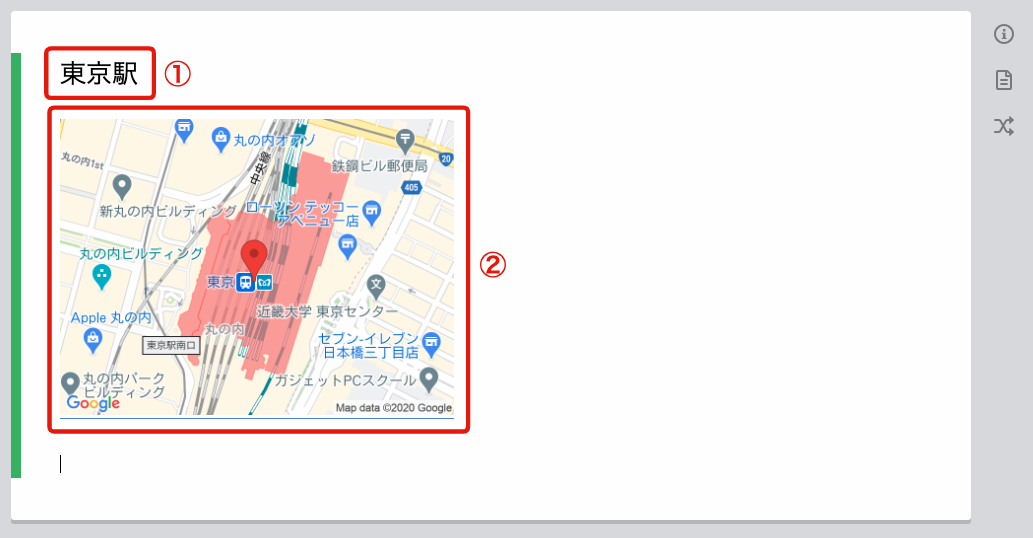
\includegraphics[width=120mm]{images/scrapbox_ar_new.png}
  \caption{新しくページを作成した時} \label{fig:scrapbox_ar_new}
\end{figure}

\paragraph*{サムネイルを追加する}
Scrapboxでは画像のURLを\texttt{[]}で囲う、または画像をドラッグ・アンド・ドロップすることで図\ref{fig:scrapbox_thumbnail}のようにページに画像を表示させることができる。
このようにScrapboxのページに画像を貼ると、ページの一番上にある画像がAR表示でのサムネイルになる。(図\ref{fig:scrapbox_thumbnail_and_ar})

\begin{figure}[H]
  \centering
  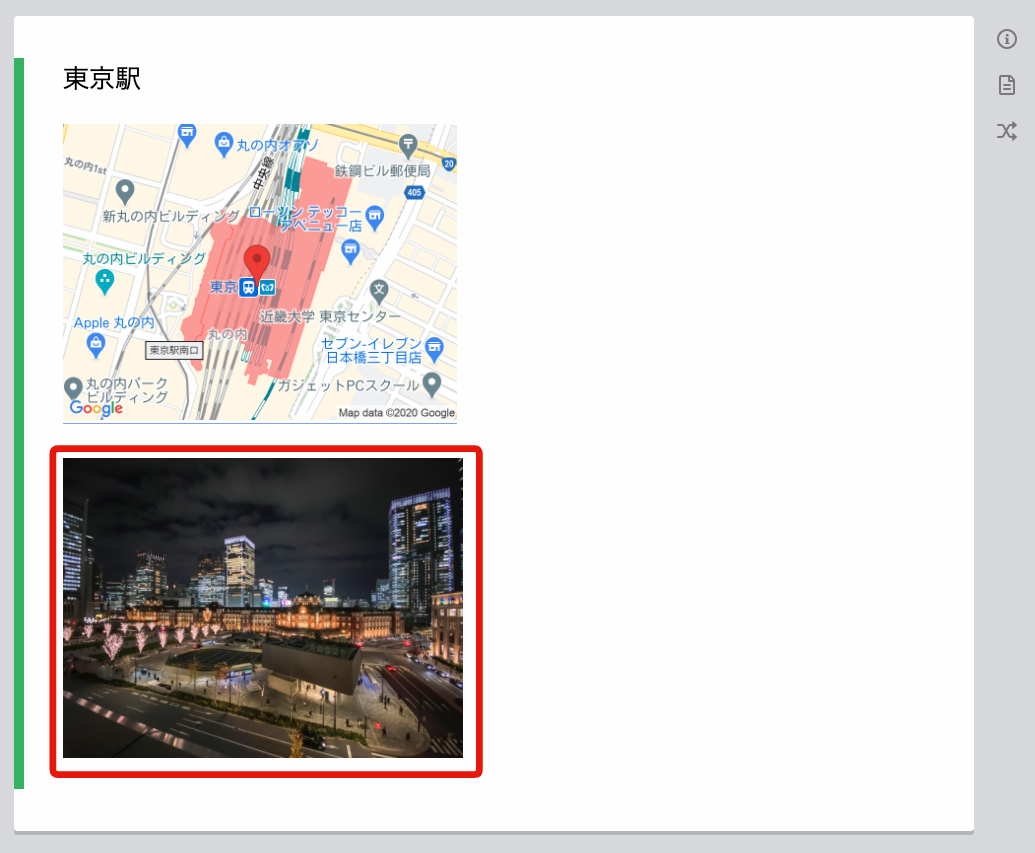
\includegraphics[width=120mm]{images/scrapbox_thumbnail.png}
  \caption{Scrapboxに貼り付けた画像} \label{fig:scrapbox_thumbnail}
\end{figure}

\begin{figure}[H]
  \centering
  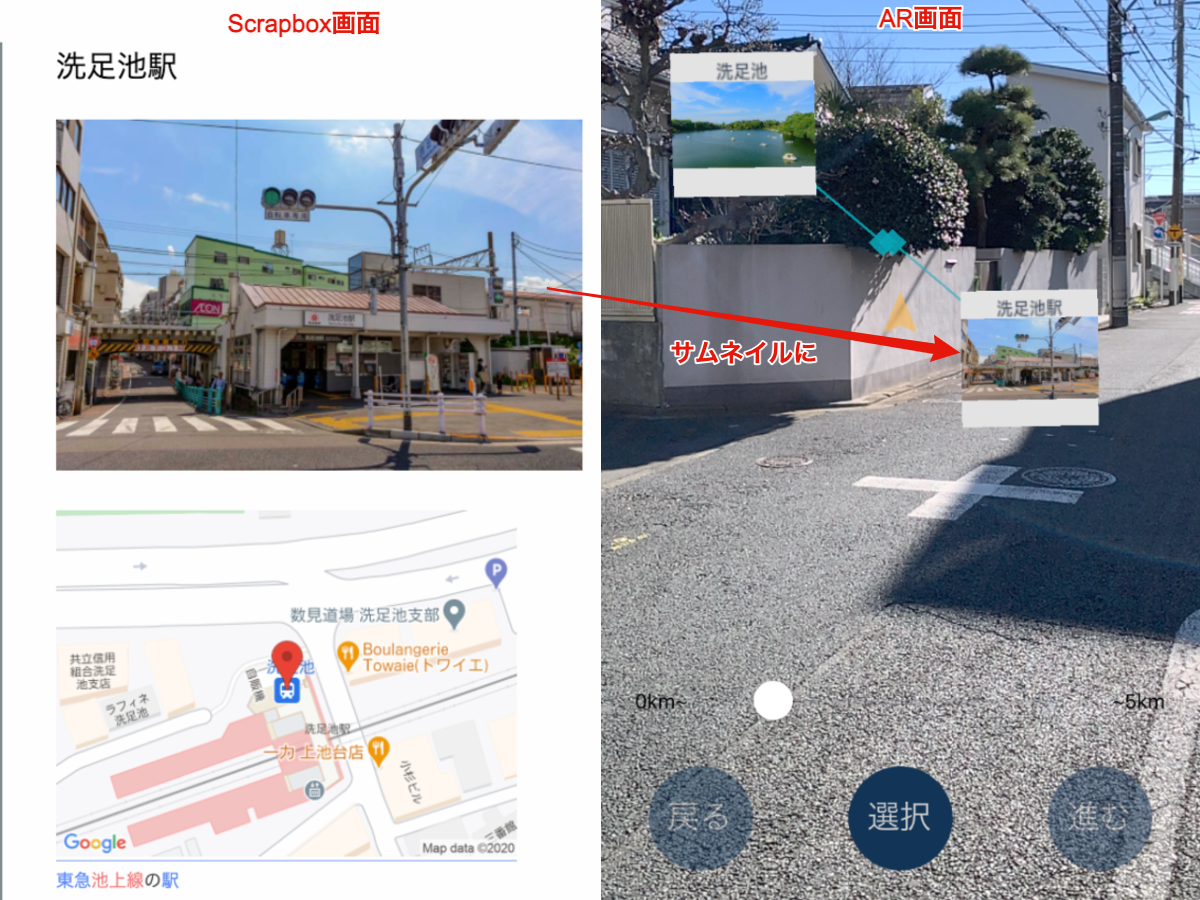
\includegraphics[width=120mm]{images/scrapbox_thumbnail_and_ar.png}
  \caption{Scrapbox上の画像とARでの表示} \label{fig:scrapbox_thumbnail_and_ar}
\end{figure}

\paragraph*{ハイパーリンクを利用して説明を書く}
Scrapboxでは単語を\texttt{[]}で囲うことにより同一Wiki内ページへのハイパーリンクとすることが可能である。
他ページヘのハイパーリンクが生成されるとAR上で関連情報として表示されるようになる(図\ref{fig:scrapbox_link_and_ar})。
ARで表示したい情報の説明を書き、説明文中の単語を積極的にハイパーリンクにすることで関連する情報を提示することができる。

\begin{figure}[H]
  \centering
  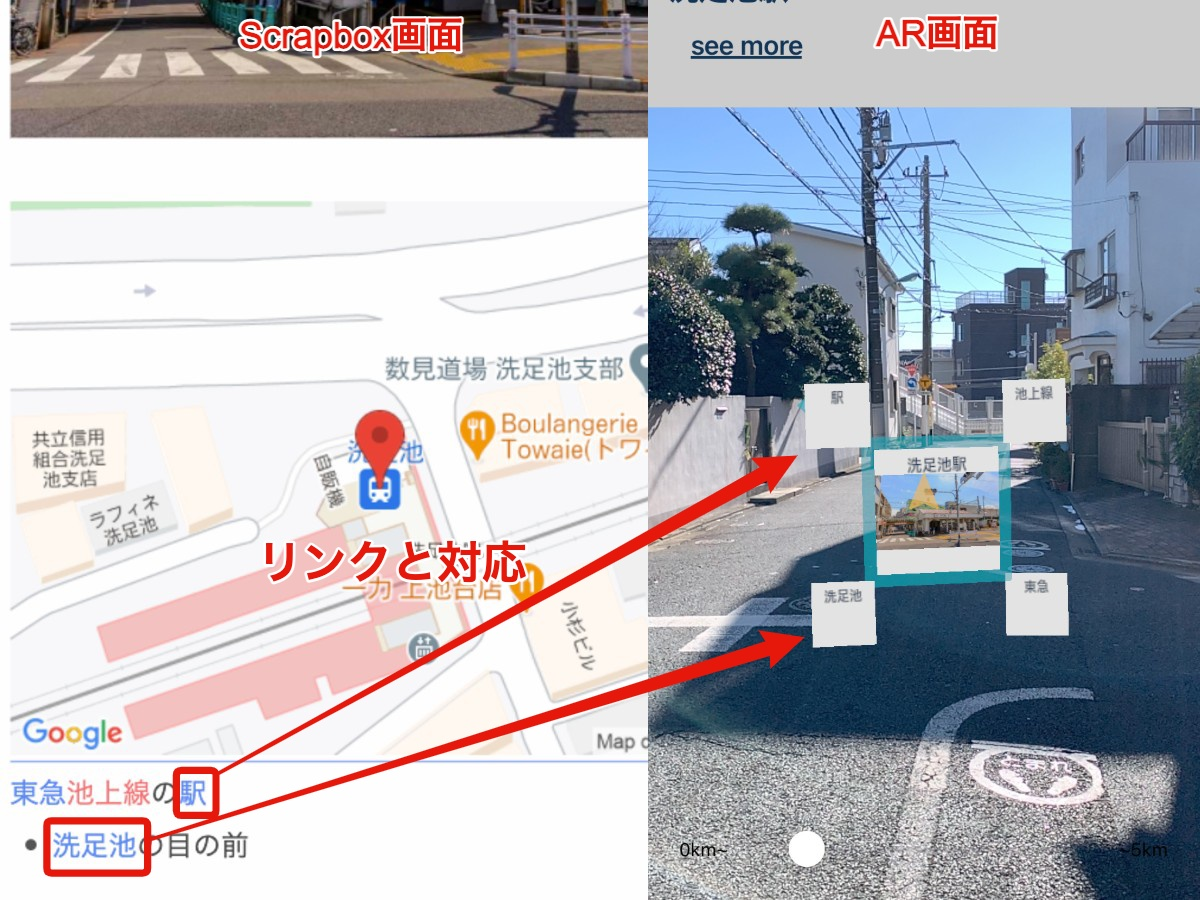
\includegraphics[width=120mm]{images/scrapbox_link_and_ar.jpg}
  \caption{Scrapbox上のリンクとARでの表示} \label{fig:scrapbox_link_and_ar}
\end{figure}

\subsubsection{NFCタグに対する情報の書き込み}
NFCタグにはISO/IEC 14443 TypeAに準拠したNTAGを利用する。
また情報を記録する際にはNFC FORUM\footnote{\textsf{https://nfc-forum.org}}によって標準化されているNDEFフォーマットで情報を書き込む。
書き込む情報は図\ref{fig:nfc_uri}のようにCustomURLSchemeに沿ったURIの形式で書き込む。

\begin{figure}[H]
  \centering
  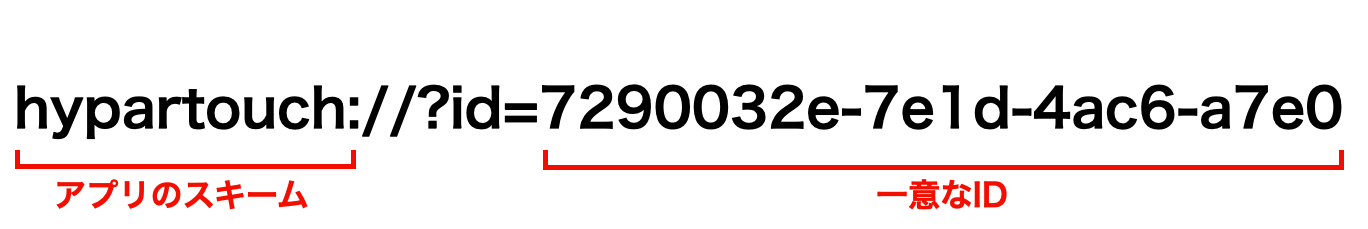
\includegraphics[width=120mm]{images/nfc_uri.png}
  \caption{NFCに書き込むURIデータ} \label{fig:nfc_uri}
\end{figure}

その上でタグに書き込んだIDと紐付ける形でHypAR Touchのサーバーに以下の情報を登録する。
\begin{itemize}
  \item 緯度経度
  \item タグの設置される向き(0〜360度)
  \item 表示するAR情報の元となるScrapboxのプロジェクト
  \item タッチした時に選択されているリンク情報
\end{itemize}
これらの情報はHypAR Touchアプリ内の登録画面(図\ref{fig:nfc_register_mobile})により登録可能である。

\begin{figure}[H]
  \centering
  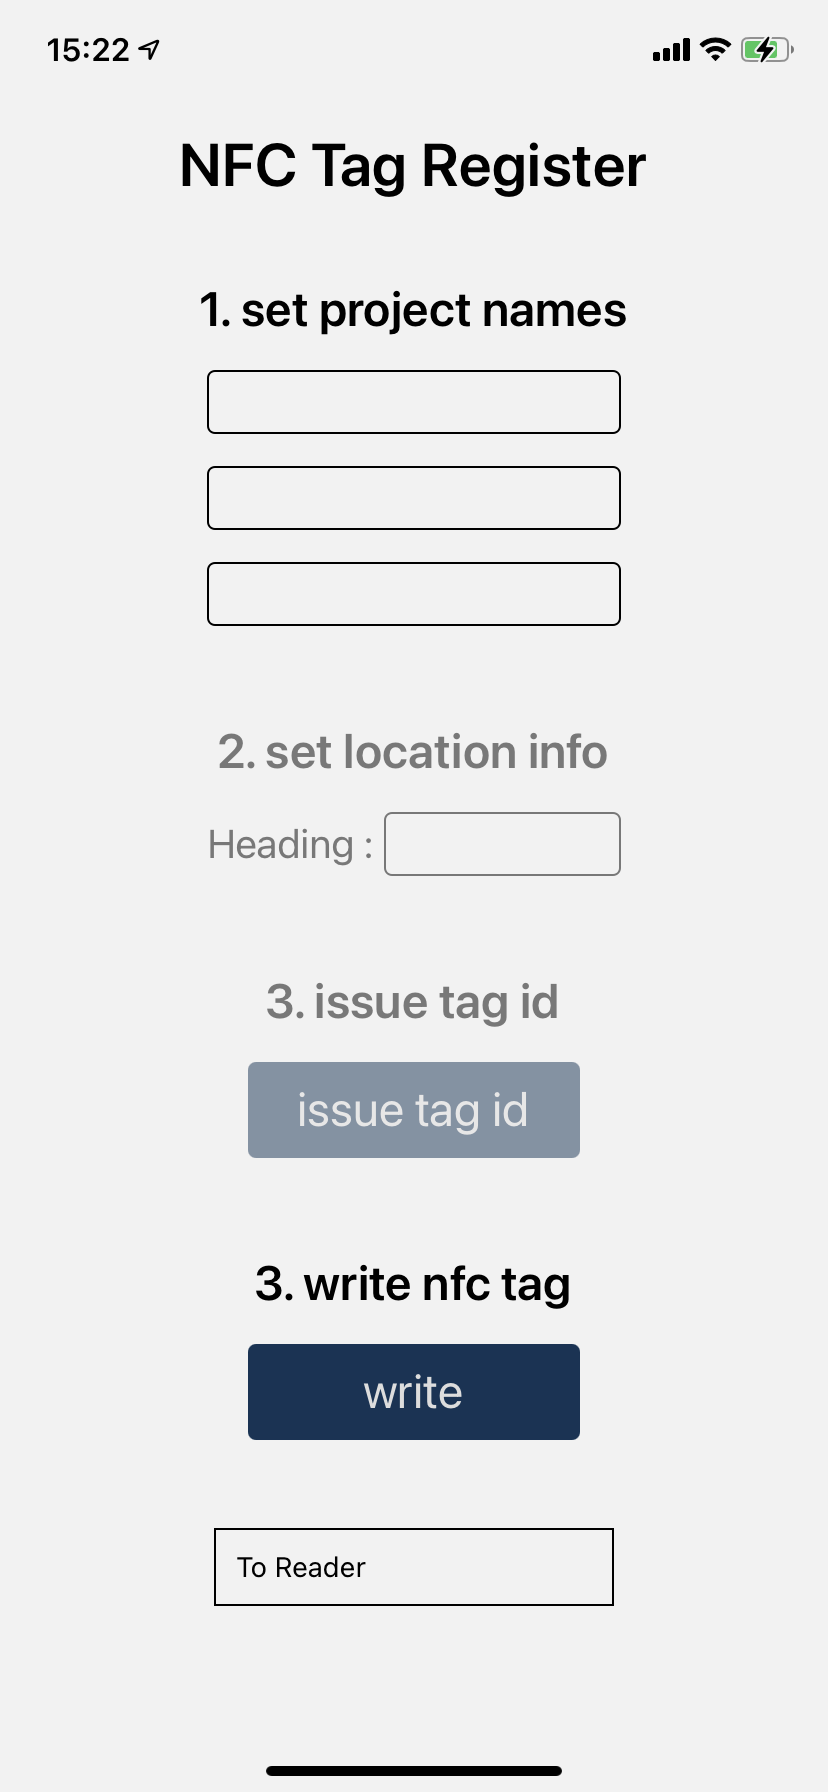
\includegraphics[height=100mm]{images/nfc_register_mobile.png}
  \caption{モバイルアプリでの登録} \label{fig:nfc_register_mobile}
\end{figure}
  % 本文4
\chapter{利用例}
\label{chap:usage}

本章では、HypAR Touchを実際に利用した様子と今後実現可能な応用例について述べる。

\newpage

\section{利用例}
HypAR Touchのプロトタイプを実際にナビゲーションシステムとして利用した際の様子を述べる。

\subsection{武蔵小杉駅及び西谷駅での利用例}
この利用例は武蔵小杉駅から相鉄・JR直通線に乗り、西谷駅で降りて昼食を取るユースケースを想定したものである。

\subsubsection{武蔵小杉駅での利用}
武蔵小杉駅は図\ref{fig:musako_2d}のようにJRと東急電鉄の駅が立体的に重なっている上に、横須賀線などJR線の一部ホームが非常に離れたところにある特殊な形をしている。
今回のユースケースでは東急電鉄の改札がある図\ref{fig:musako_2d}の\textcircled{\scriptsize{1}}からスタートし、\textcircled{\scriptsize{2}}のJR改札口を通り\textcircled{\scriptsize{3}}のホームまで向かう。

まずは\textcircled{\scriptsize{1}}の地点で利用した様子を述べる。
図\ref{fig:musako_tokyu_ar1}は\textcircled{\scriptsize{1}}から\textcircled{\scriptsize{2}}の方向を見た時の様子である。
\textcircled{\scriptsize{2}}の方向には「武蔵小杉駅」の表記があり、表記の奥にあるエスカレータを登ることで\textcircled{\scriptsize{2}}の改札に到達できることがわかる。
また図\ref{fig:musako_tokyu_ar2}は\textcircled{\scriptsize{1}}から正面(図\ref{fig:musako_2d}の上方向)を見たときの様子である。
正面に「武蔵小杉駅南武線ホーム」という表示があるように、その方向には\textcircled{\scriptsize{2}}から階段を降りた南武線のホームがある。
今回のユースケースでは南武線に乗らなかったが、南武線に乗り換える場合はこの場所に南武線のホームがある事がわかるため乗り換えの際、他のホームと間違える可能性が少なくなると考えられる。

\begin{figure}[H]
  \centering
  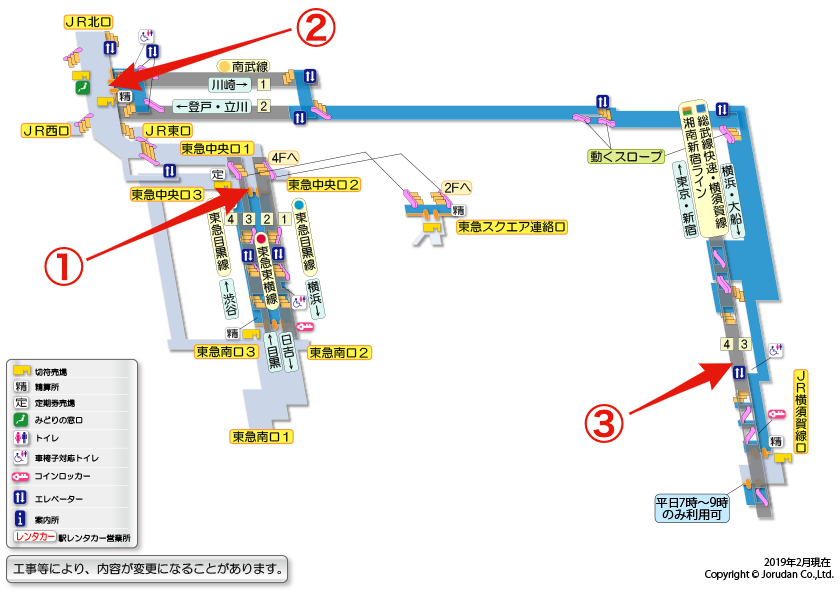
\includegraphics[width=120mm]{images/musako_2d.png}
  \caption{武蔵小杉駅の構内図} \label{fig:musako_2d}
\end{figure}
\begin{figure}[H]
  \begin{minipage}{0.5\hsize}
    \centering
    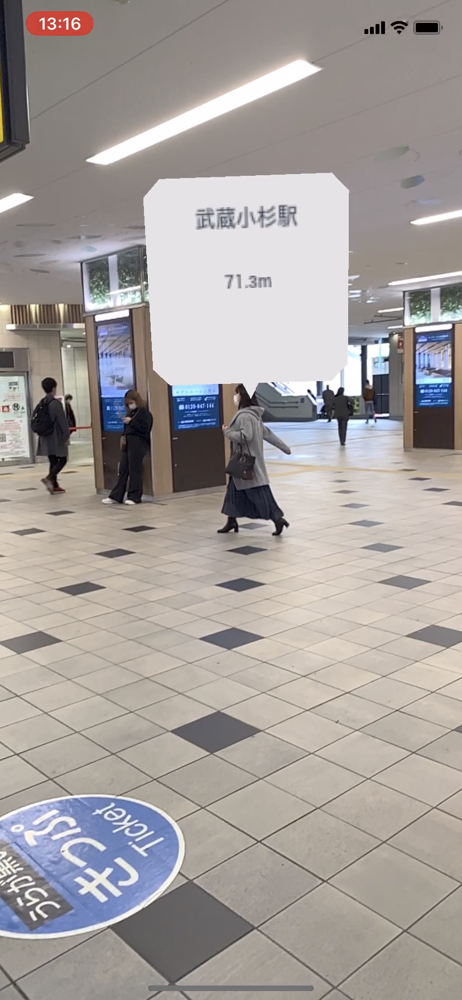
\includegraphics[height=100mm]{images/musako_tokyu_ar1.png}
    \caption{地点\textcircled{\scriptsize{1}}から\textcircled{\scriptsize{2}}を見た時} \label{fig:musako_tokyu_ar1}
  \end{minipage}
  \begin{minipage}{0.5\hsize}
    \centering
    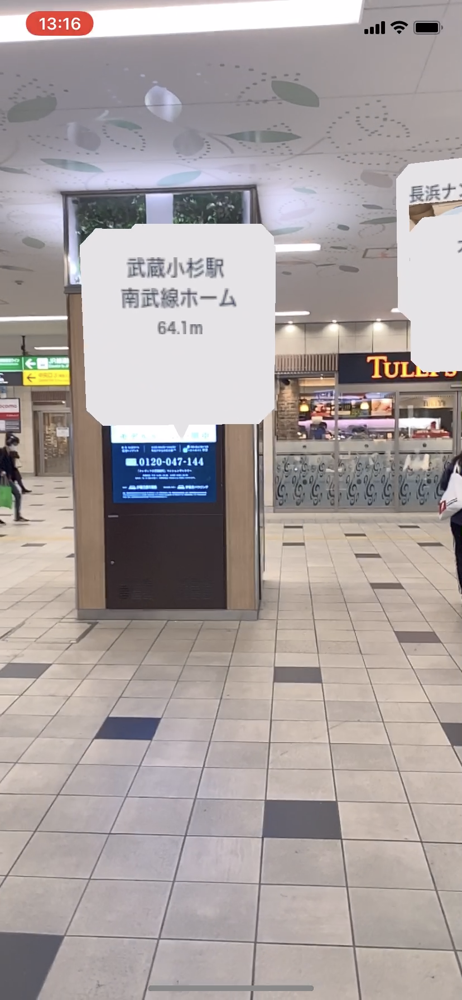
\includegraphics[height=100mm]{images/musako_tokyu_ar2.png}
    \caption{地点\textcircled{\scriptsize{1}}から正面を見た時} \label{fig:musako_tokyu_ar2}
  \end{minipage}
\end{figure}

次に図\ref{fig:musako_2d}の\textcircled{\scriptsize{2}}の地点で本システムを使用した様子を述べる。
図\ref{fig:musako_jr_ar1}は\textcircled{\scriptsize{2}}の地点から\textcircled{\scriptsize{3}}の位置を見ている時の様子である。
距離の表示で402mとあるように横須賀線のホームが改札奥右側の階段を降りた先にあることがわかる。
実際に横須賀線のホームに向かうためには改札奥右側の階段を降りる必要がありこの表示が正しいことがわかる。
\begin{figure}[H]
  \centering
  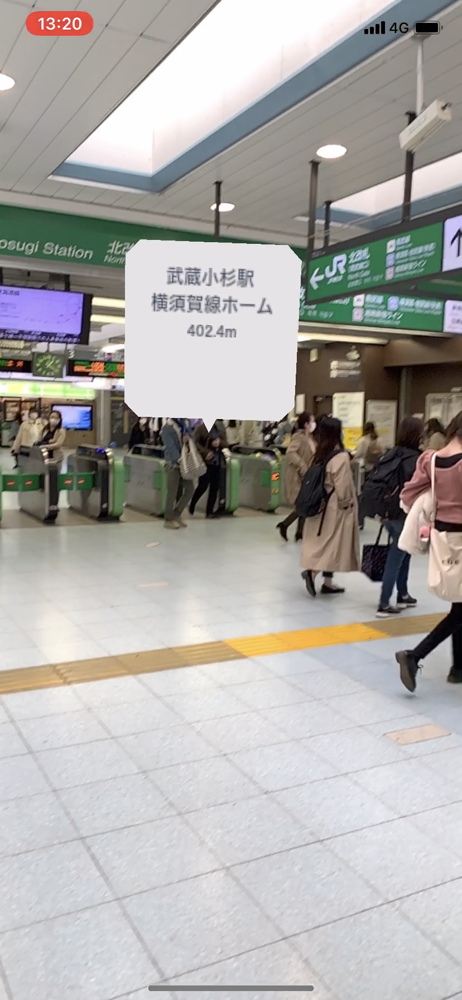
\includegraphics[height=100mm]{images/musako_jr_ar1.png}
  \caption{リンクを利用したルートの表記例} \label{fig:musako_jr_ar1}
\end{figure}
このように武蔵小杉駅での利用例から、ARで正しい位置に案内表示が出ることで複雑な構造の駅でも悩まず乗り換えができることが分かる。


\subsubsection{西谷駅での利用}
次に、西谷駅の近くで飲食店をさがすために本システムを利用した。
知らない土地での利便性を確かめるため、筆者が一度も訪れたことがなく土地勘のない西谷駅を選択した。
また西谷駅付近の飲食店の情報は西谷駅周辺に住む研究室の学生の情報を元に入力した。

西谷駅は図\ref{fig:nishiya_2d}のような比較的単純な形をしている。今回は改札を出た図\ref{fig:nishiya_2d}の\textcircled{\scriptsize{1}}の地点で本システムを利用した。
図\ref{fig:nishiya_maruichi_ar}は図\ref{fig:nishiya_2d}の\textcircled{\scriptsize{1}}の位置から矢印方向にモバイル端末を向けた上で、「丸一」というAR情報を選択したときの様子である。
選択されたAR情報の周辺には関連リンクである「ラーメン」、「家系」、「西谷駅」の3つが表示されている。
このようなリンク情報とサムネイルからこのお店は家系と呼ばれる種類のラーメン屋であり西谷駅の近くにあることがわかる。
また関連リンクのうち「ラーメン」を選択したときの様子が図\ref{fig:nishiya_ramen_ar}である。
表示される情報が「ラーメン」というリンクが含まれるAR情報に絞られ、実際に付近のラーメン屋である「丸一」、「北海ラーメン 蝦夷」、「麺屋奨 TASUKU」が表示されている。
さらに図\ref{fig:nishiya_ezo_ar}は付近のラーメン屋である「北海ラーメン 蝦夷」を選択した時の様子である。
サムネイルからラーメンの様子がわかるだけでなく、「生姜焼き」と言うリンクから生姜焼きが有名であることがわかる。
今回の利用では最終的に「北海ラーメン 蝦夷」に向かうことにしたが、既にARの表示から図\ref{fig:nishiya_2d}の矢印の方向160mにあることが分かっているので図nの\textcircled{\scriptsize{2}}の出口から道沿いに進むだけで実際に店にたどり着くことができた。

西谷駅での利用例から、本システムは以下のように利用できることが分かった。
\begin{itemize}
  \item 付近のお店を探すことができる。
  \item リンク情報からお店の系統や有名なメニューを知ることができる。
  \item リンク情報をもとに同じ種類の店一覧を見ることができる。
\end{itemize}
このように探索的なナビゲーションがARで表示されることによって、自身の全く知らない場所でも迷いなく店を比較検討し、実際に訪れることができた。

\begin{figure}[H]
  \centering
  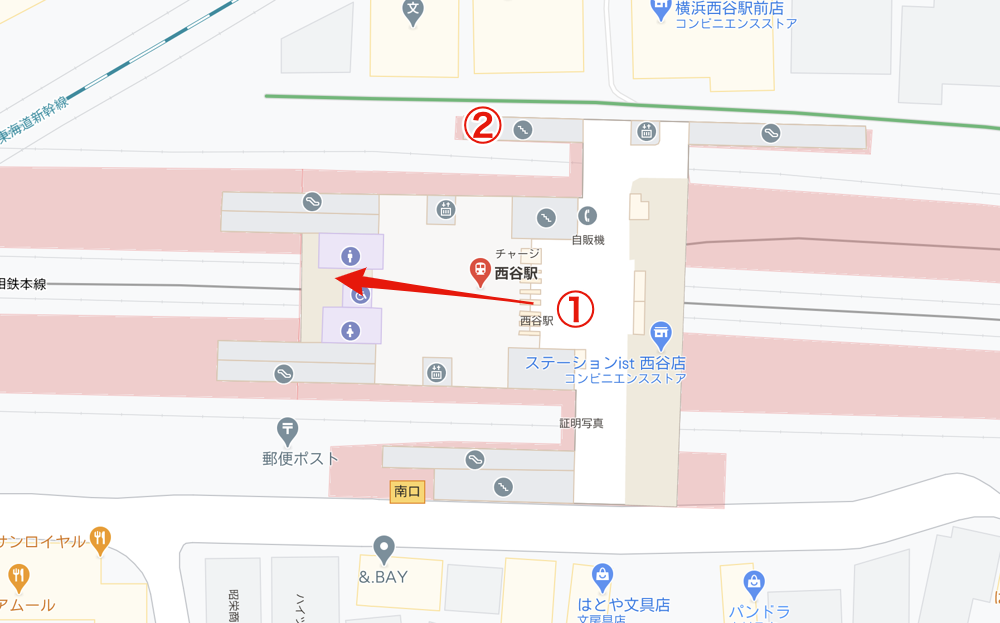
\includegraphics[width=120mm]{images/nishiya_2d.png}
  \caption{西谷駅の構内図} \label{fig:nishiya_2d}
\end{figure}

\begin{figure}[H]
  \begin{minipage}{0.5\hsize}
    \centering
    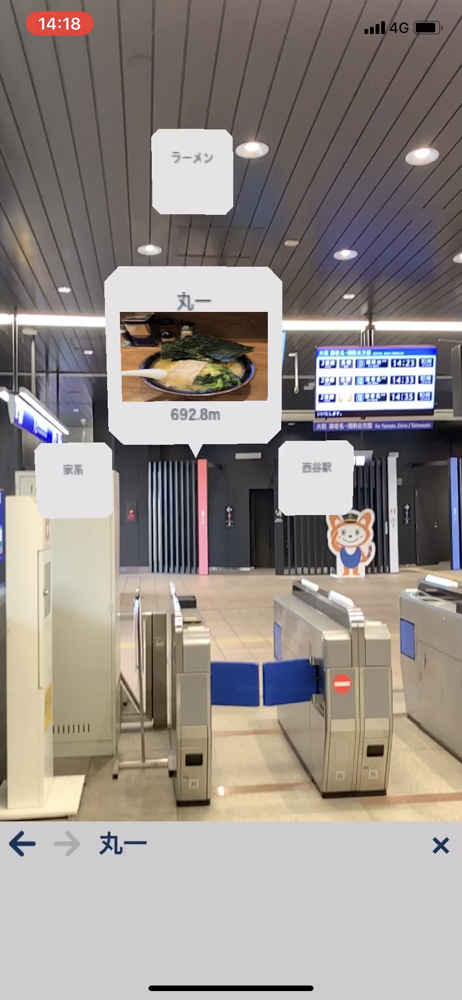
\includegraphics[height=100mm]{images/nishiya_maruichi_ar.png}
    \caption{「丸一」を選択した時} \label{fig:nishiya_maruichi_ar}
  \end{minipage}
  \begin{minipage}{0.5\hsize}
    \centering
    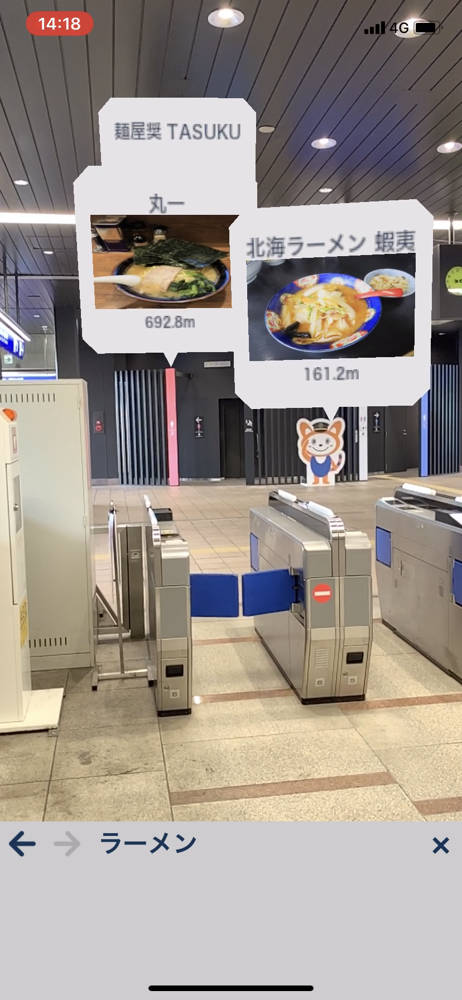
\includegraphics[height=100mm]{images/nishiya_ramen_ar.png}
    \caption{「ラーメン」というリンクを選択した時} \label{fig:nishiya_ramen_ar}
  \end{minipage}
\end{figure}

\begin{figure}[H]
  \centering
  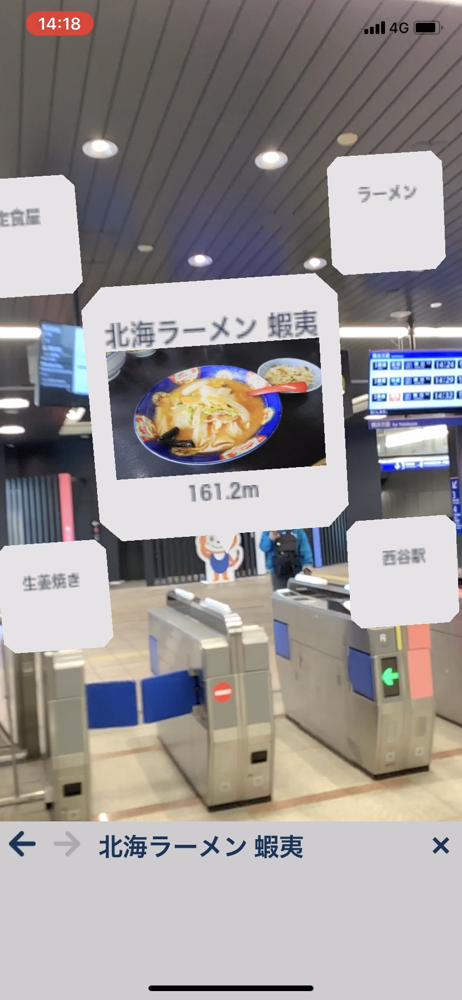
\includegraphics[height=100mm]{images/nishiya_ezo_ar.png}
  \caption{「北海ラーメン 蝦夷」を選択した時} \label{fig:nishiya_ezo_ar}
\end{figure}


\subsection{湘南台での利用例}
この利用例は湘南台の小田急改札から本システムを利用してSFCに向かうバスに乗るユースケースを想定したものである。

図\ref{fig:shonandai_bus_exit1}は湘南台駅の小田急改札前で西側を向いたときの本システムの様子である。
この時点で西方向にはARで「西口バスのりば」の表示が出ている。
さらにこの情報を選択した状態が図\ref{fig:shonandai_bus_exit_selected}である。
ここでは関連リンク情報として「バス」「バスのりば」「SFC」の3つが表示されている。
このことからこのバス乗り場がSFCに向かうバス停であることがわかる。
このAR情報は「SFC」という単語から検索を行っても関連情報として表示されるので、SFCにはじめて来るユーザでも迷うことなくバス停の場所がわかる。

さらにこのAR情報を選択した状態で移動ボタンを押し、バス停付近に視点を移動させた時の様子が図\ref{fig:shonandai_bus_moved}である。
今回の例のようにユーザが地下におり、目的地である地上の様子がわからない時などはこの視点移動機能で現地の様子を確認することができる。
この機能により万が一目的地付近で迷っても、目的地視点の情報から正しく目的地に到達できる。

また図\ref{fig:shonandai_bus2}はバス停から遠い地上出口から案内を見た時の様子である。
この場合も図\ref{fig:shonandai_bus_exit1}同様にバス停の位置を正しく表示している。
本システムはアプリの起動や案内がタグへのタッチだけで行なえるため、少しでも経路が不安になったら付近のタグにタッチして目的地の場所を再確認する事ができる。

このようにタッチというインタラクションだけで新しい案内に更新できる本システムは地理感覚のない土地での案内として非常に有用である。


\begin{figure}[H]
  \begin{minipage}{0.5\hsize}
    \centering
    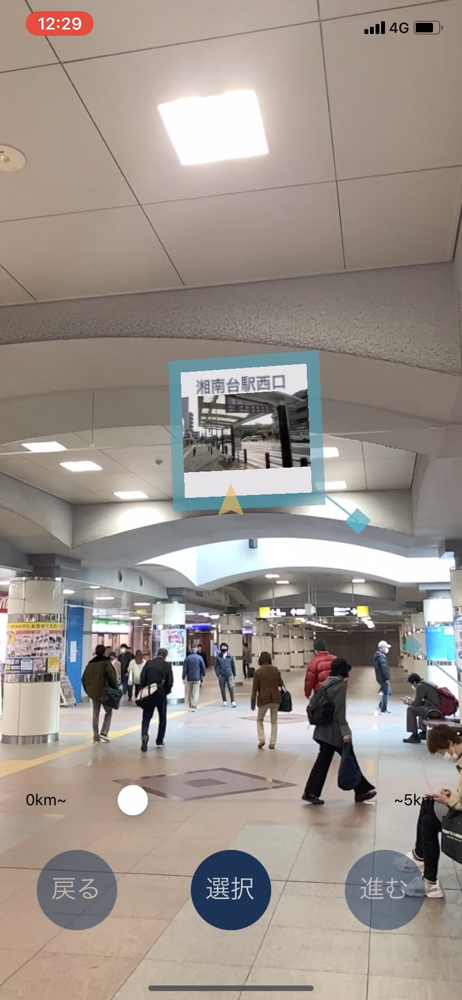
\includegraphics[height=100mm]{images/shonandai_bus_exit1.png}
    \caption{湘南台駅(地下)からの案内} \label{fig:shonandai_bus_exit1}
  \end{minipage}
  \begin{minipage}{0.5\hsize}
    \centering
    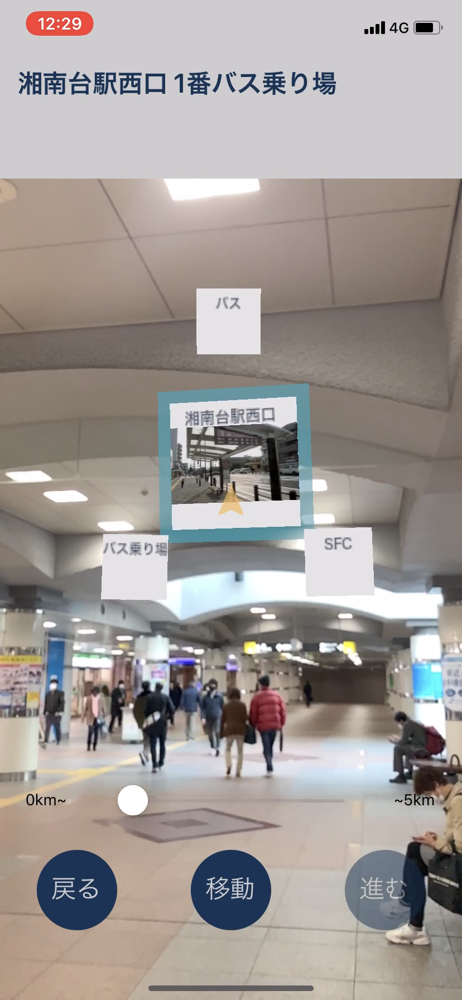
\includegraphics[height=100mm]{images/shonandai_bus_exit_selected.png}
    \caption{バス停の情報を選択した時} \label{fig:shonandai_bus_exit_selected}
  \end{minipage}
\end{figure}

\begin{figure}[H]
  \begin{minipage}{0.5\hsize}
    \centering
    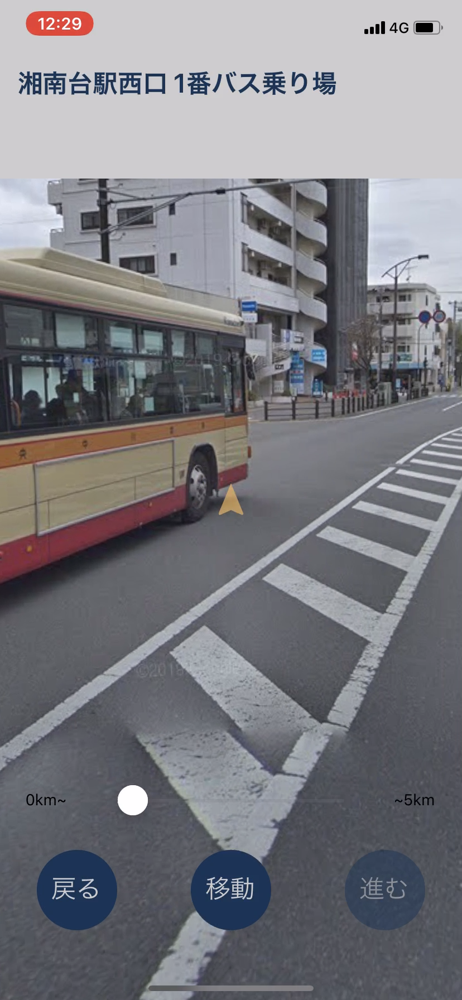
\includegraphics[height=100mm]{images/shonandai_bus_moved.png}
    \caption{バス停付近からの視点} \label{fig:shonandai_bus_moved}
  \end{minipage}
  \begin{minipage}{0.5\hsize}
    \centering
    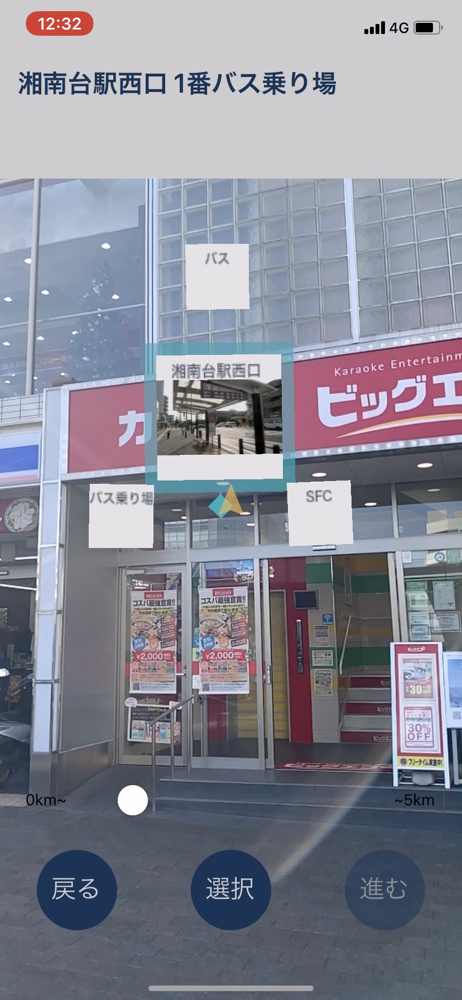
\includegraphics[height=100mm]{images/shonandai_bus2.png}
    \caption{地上出口からの案内} \label{fig:shonandai_bus2}
  \end{minipage}
\end{figure}


\section{応用例}
前節での実際の利用を踏まえ考えられる利用例及び応用例をまとめ、その利点を記載する。

\subsection{駅など公共施設での案内}
駅や空港などの比較的大規模な公共施設内ではGPSによる案内が利用できない場合が多く、2次元の地図を提示するか矢印などによる案内表示を行うのが一般的である。
しかしながら両者にはそれぞれ案内システムとして問題が存在する。

2次元の地図は内部構造が複雑な屋内を表現することが難しく、地下鉄ホームなどの複雑な地形の案内に不向きである。
また設置できる場所に限りがあり、必要な時に参照できないことがある。
矢印などによる案内表示の場合、記述できる情報に限りがあり、必ずしも自分の目的地に沿う案内があるとは限らないという問題点がある。

これらの従来の案内システムと比べ、本システムではARで目的地を直接提示(図:\ref{fig:ar_navigation_shonandai})するため地図の苦手な人への案内や複雑な構造の施設の案内において有用である。
またNFCタグは一枚あたり十数円と安価で、サイズも小さいため設置場所やコストに困るケースは少ないといえる。
さらにNFCタグに紐付いた情報により表示するAR情報のあるScrapboxプロジェクトやハイパーリンクによるフィルターを指定できる。
そのため駅の出口だけを案内したり(図:\ref{fig:ar_navigation_exit})広告として特定店舗だけを案内したり(図:\ref{fig:ar_navigation_ad})といった特定の用途に特化した案内をすることも可能である。

\begin{figure}[H]
  \centering
  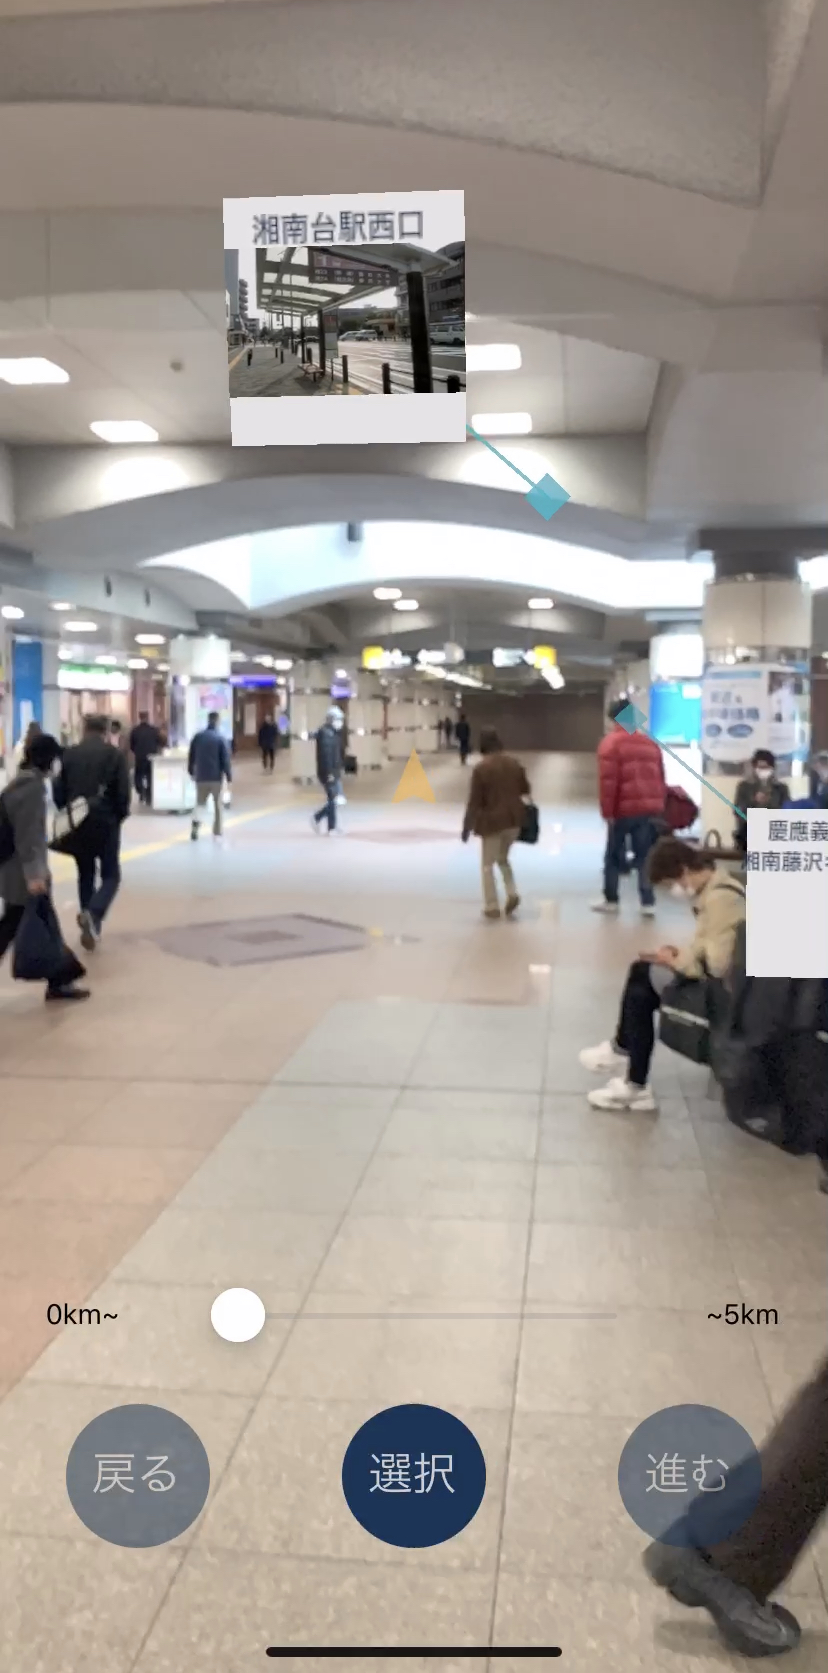
\includegraphics[height=100mm]{images/ar_navigation_shonandai.jpg}
  \caption{案内の様子} \label{fig:ar_navigation_shonandai}
\end{figure}

\begin{figure}[H]
  \centering
  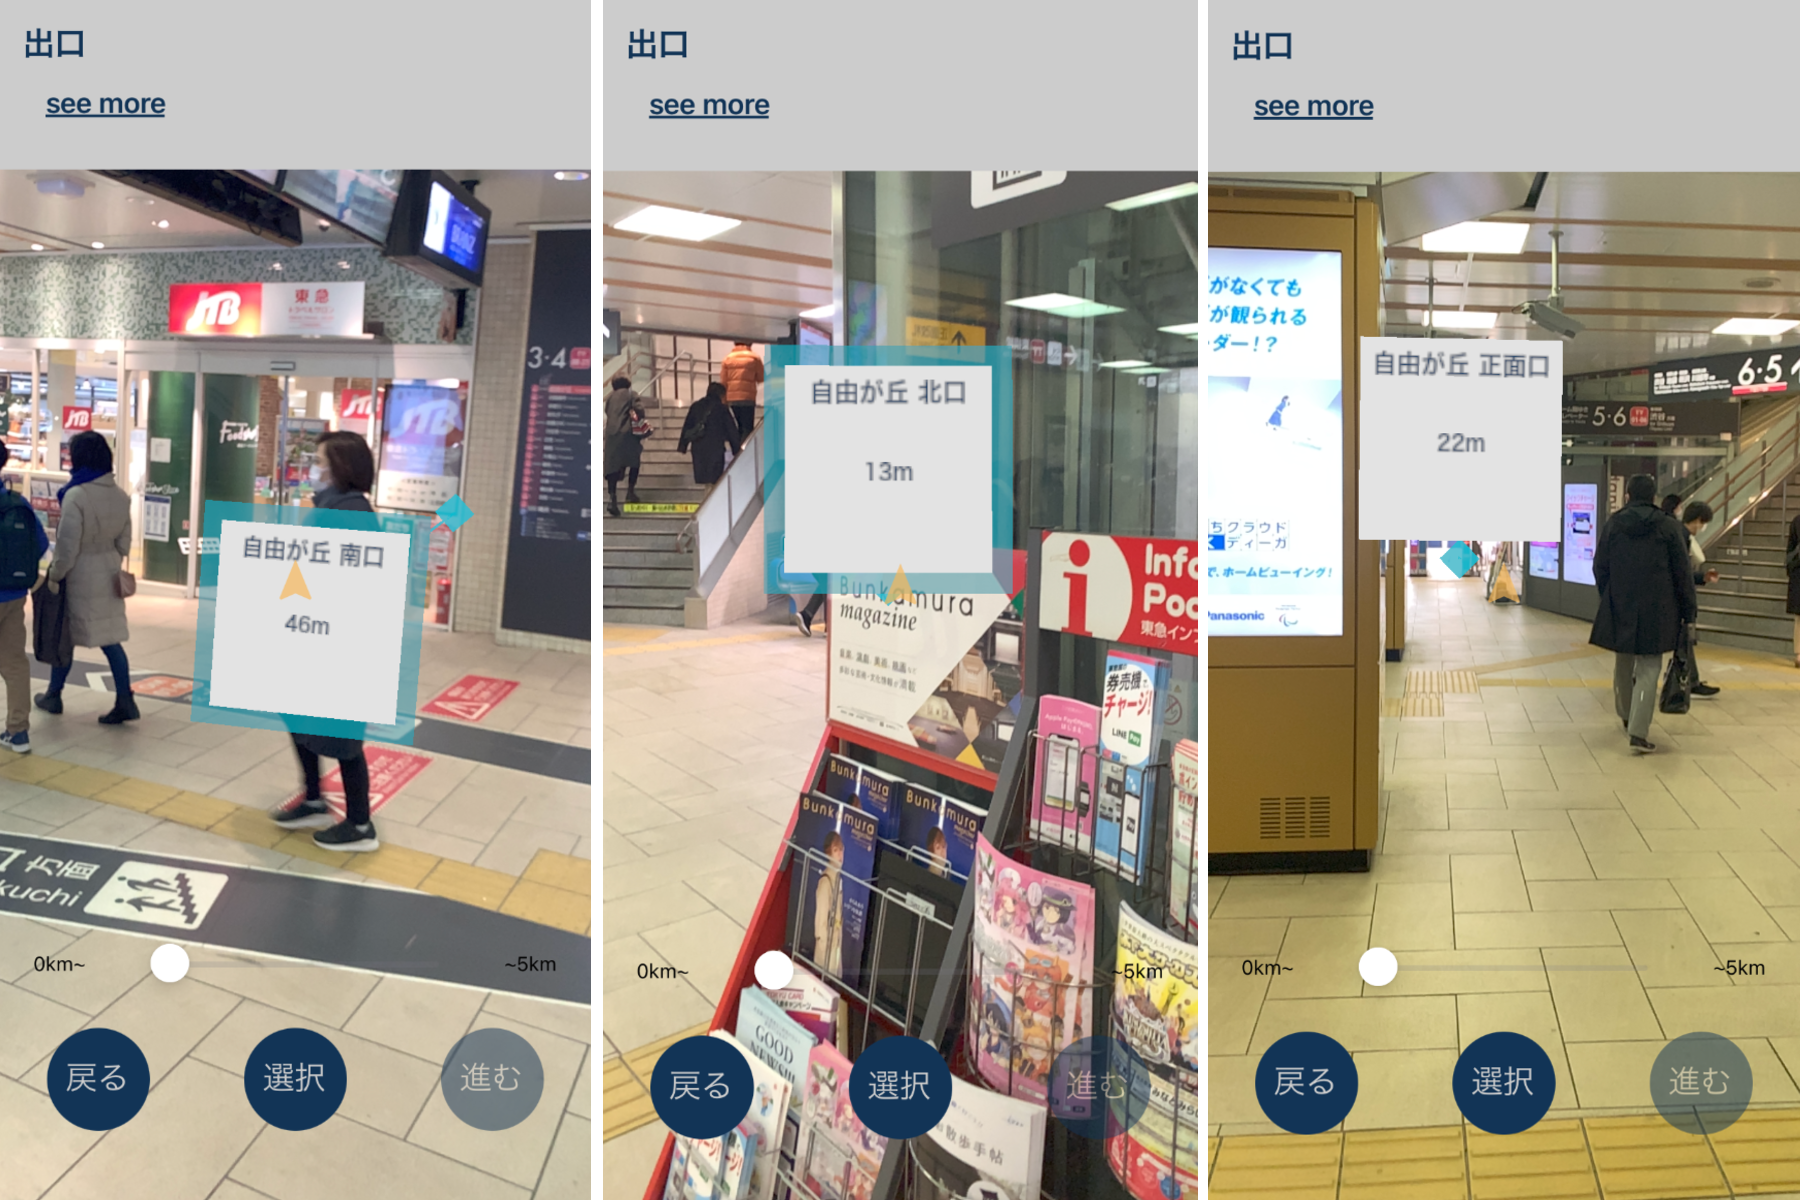
\includegraphics[width=120mm]{images/ar_navigation_exit.png}
  \caption{出口だけの案内} \label{fig:ar_navigation_exit}
\end{figure}

\begin{figure}[H]
  \centering
  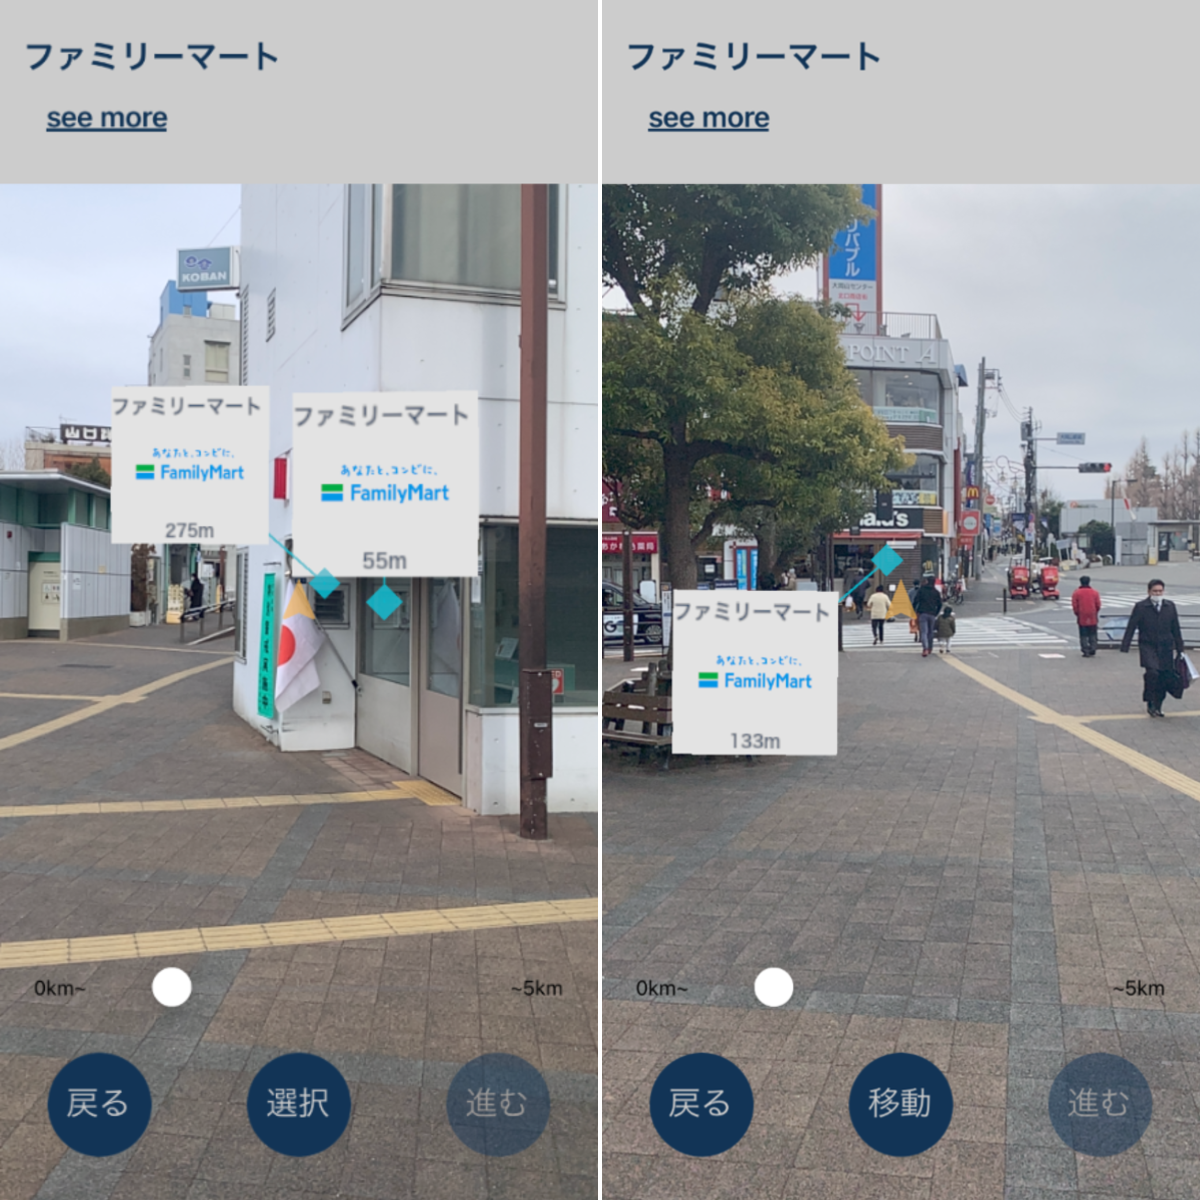
\includegraphics[height=100mm]{images/ar_filter_famima.png}
  \caption{コンビニだけをフィルタした様子} \label{fig:ar_navigation_ad}
\end{figure}

\subsection{近隣施設の探索・推薦}

本システムの大きな特徴としてWikiを利用することにより情報を階層化せずに関連情報を参照できる点が挙げられる。
その結果以下のような探索がAR上で行える
\begin{itemize}
  \item 近隣施設の情報にあるリンクから関連情報を参照する
  \item 関連情報から興味のあるジャンルの店舗を発見する
  \item 履歴機能を使いながらほかの情報を比較する
\end{itemize}
上記のような能動的探索行為は目的地への案内のみを目的としている既存のアプリケーションでは体験できないものである。


例として神保町のように様々な分野の店舗情報が登録される可能性が高い地域で本システムを利用する例を考える。
本システムのユーザが神保町にウィンタースポーツ用品を買いに来ていたと仮定する。

神保町には多くのウィンタースポーツ用品店があるため、これらを比較しながら巡りたいと考える可能性は高い。
このような場合ARでの表示情報からウィンタースポーツ用品店を選択すれば、「スノーボード」「スキー」といったいったリンクが出現する(図\ref{fig:ar_navigation_jibotyo_ski})。
ウィンタースポーツ用品店をめぐりたい場合はこれらのリンクを選択することで各店舗を比較しながら見ることができる。

その後同じく神保町で食事をを取りたいと考えたとする。
本システムではウィンタースポーツ用品店の情報も飲食店の情報もおなじWikiプロジェクトに含まれているため先程とおなじタグから飲食店の探索ができる。
実際に、興味のある飲食店を選択する(図\ref{fig:ar_navigation_jibotyo_lunch})ことで「ラーメン」「カレー」等のリンクが出現し、自身の食べたいものを絞り込み(図\ref{fig:ar_navigation_jibotyo_link})、他の店舗と比較しながら探索できる。

このように本システムは様々な施設の情報が混在していてもリンクを選択していくことで自分の求める情報を探索でき、既存のARナビゲーションアプリにない魅了を持った非常に拡張性の高いシステムであると言える。


\begin{figure}[H]
  \begin{minipage}{0.5\hsize}
    \centering
    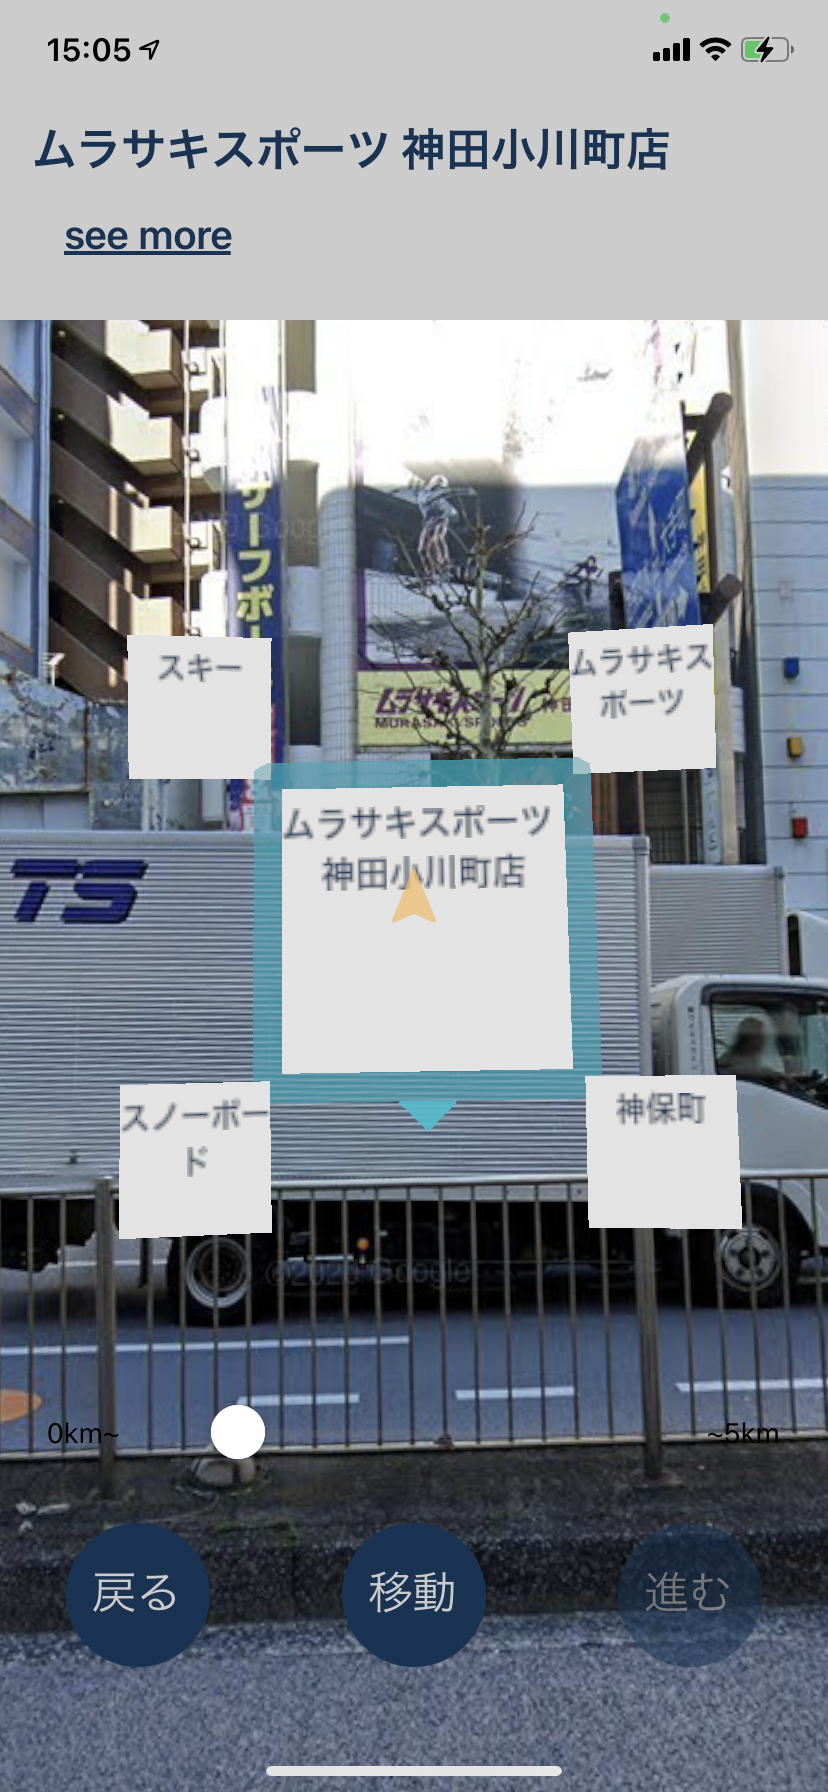
\includegraphics[height=100mm]{images/ar_navigation_jibotyo_ski.png}
    \caption{スキーのリンクを選択した時のイメージ} \label{fig:ar_navigation_jibotyo_ski}
  \end{minipage}
  \begin{minipage}{0.5\hsize}
    \centering
    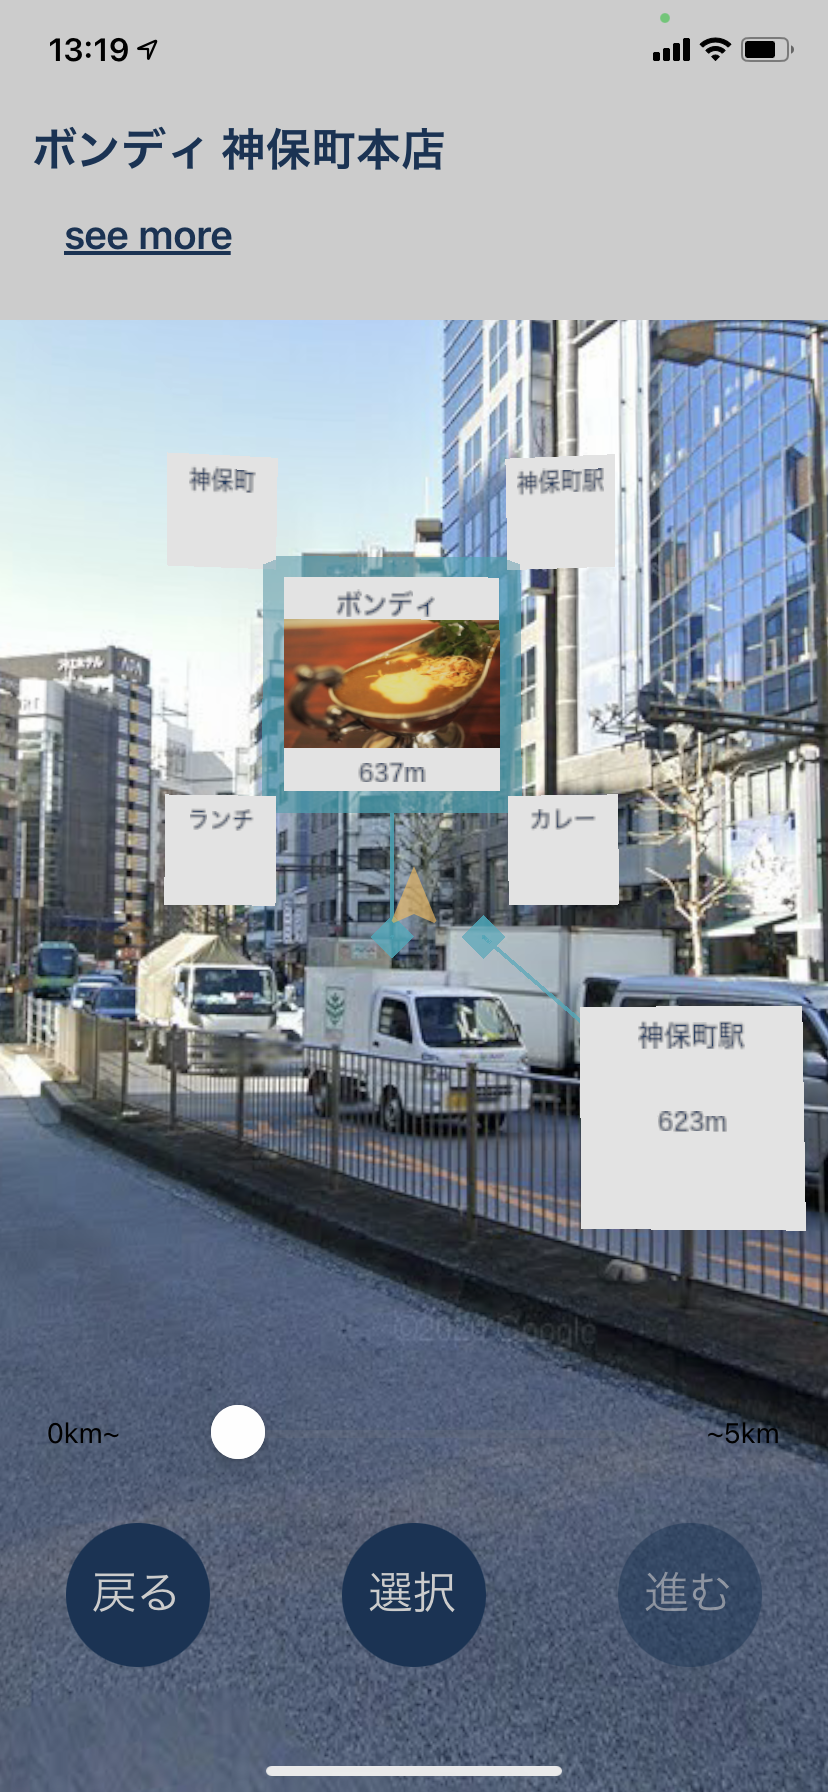
\includegraphics[height=100mm]{images/ar_navigation_jibotyo_lunch.png}
    \caption{飲食店を選択した時のイメージ} \label{fig:ar_navigation_jibotyo_lunch}
  \end{minipage}
\end{figure}

\begin{figure}[H]
  \centering
  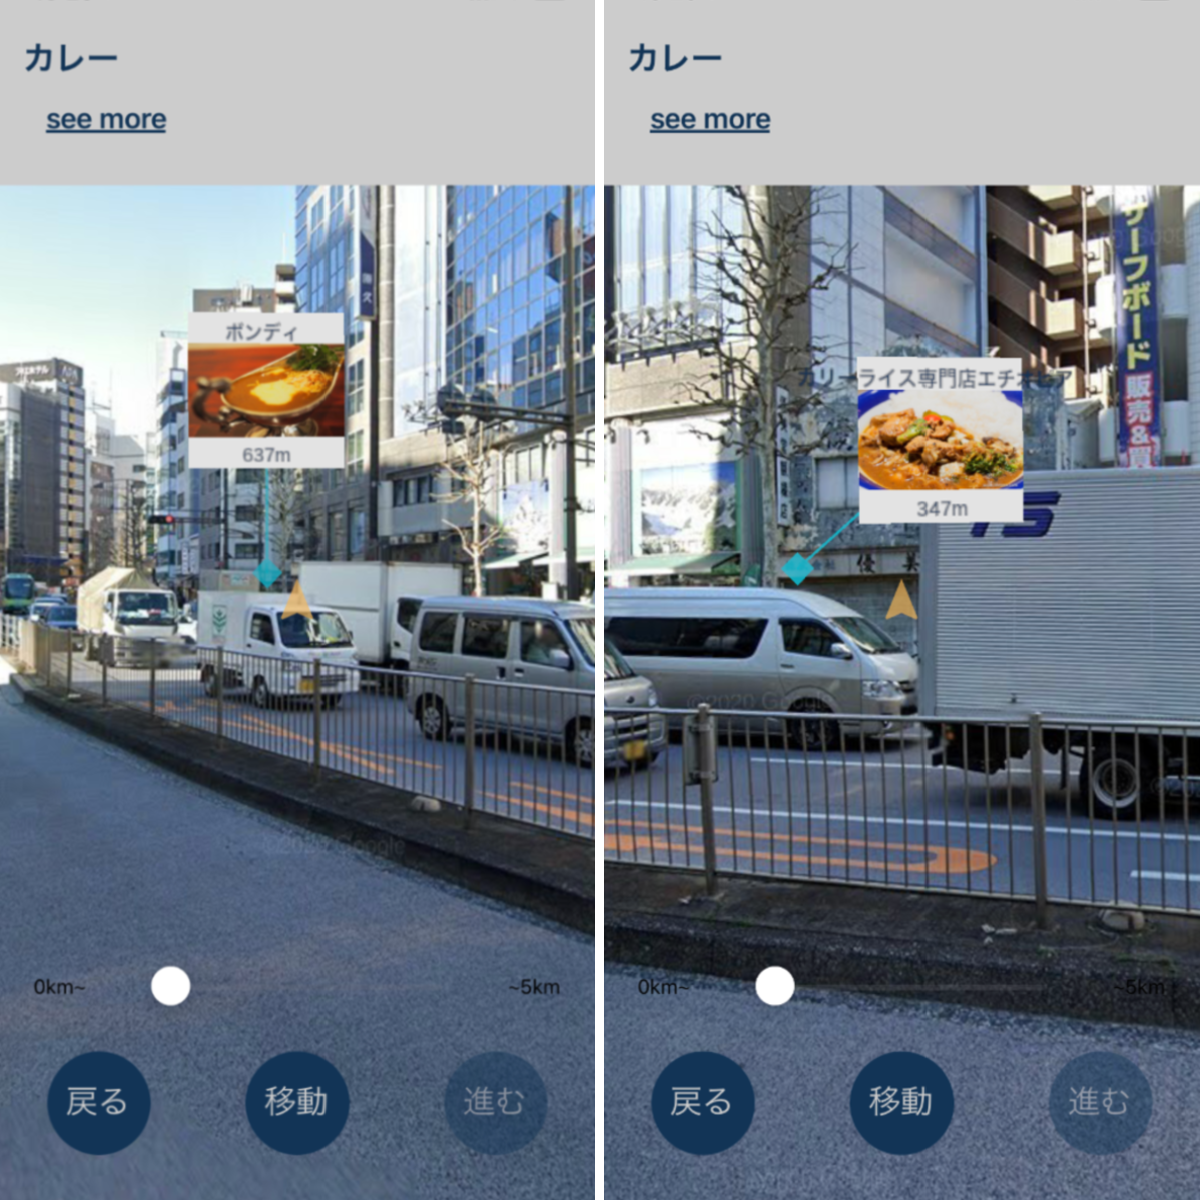
\includegraphics[width=100mm]{images/ar_navigation_jibotyo_link.png}
  \caption{カレーで絞り込みをしている様子} \label{fig:ar_navigation_jibotyo_link}
\end{figure}


\subsection{学習教材としての利用}
WikiはWikipediaに代表されるように膨大な史実や地理情報を整理し、記録するのに適したメディアであると言える。
本システムではWikiの各ページに位置情報を記載するだけでARでの表示が行えるため、地理情報を多く含む歴史学や地理学の教材として利用するのに適している。

例として京都など史跡が多い地域でのフィールドワークに利用する例が考えられる。
学習者は各地にあるタグに触れるだけで周辺にある史跡の情報見ることができるだけでなく、選択した史跡の関連情報から他の史跡の情報や位置をARで見ることができる。
これにより自身の興味や学習対象に関連する史跡を効率よく回り、自身の知らない史跡を知る事ができる。

さらに本システムでは第3章で述べた通り現在地からのAR表示だけでなく選択されたAR情報の場所に視点を移動する事が可能である。
この機能によって現地に行かなくても関連情報をたどって視点を切り替えながら史跡を見ることが可能である。

教育現場などでこの視点移動機能を利用すれば、実際の景色や建造物を見ながら史跡や史実の学習をすることができる。

一例として日本史上の事件である、禁門の変について学んでいると仮定した際の例を考える。
図\ref{fig:ar_kinmon}のように「禁門の変」というページを選択するとこの事件に関連のある場所が表示される。
表示された情報を選択すると今度はその場所の情報を見ることができる(図\ref{fig:ar_yashiki})。


またAR情報の編集環境としてWikiシステムであるScrapboxを採用しているため先生や学生が内容を登録したり加筆することも容易である.
アクティブラーニングの推進が求められている中、学生が主体的に情報をまとめながら地理的理解とともに学習を行える本システムは学習体験を大きく向上することができる。


\begin{figure}[H]
  \centering
  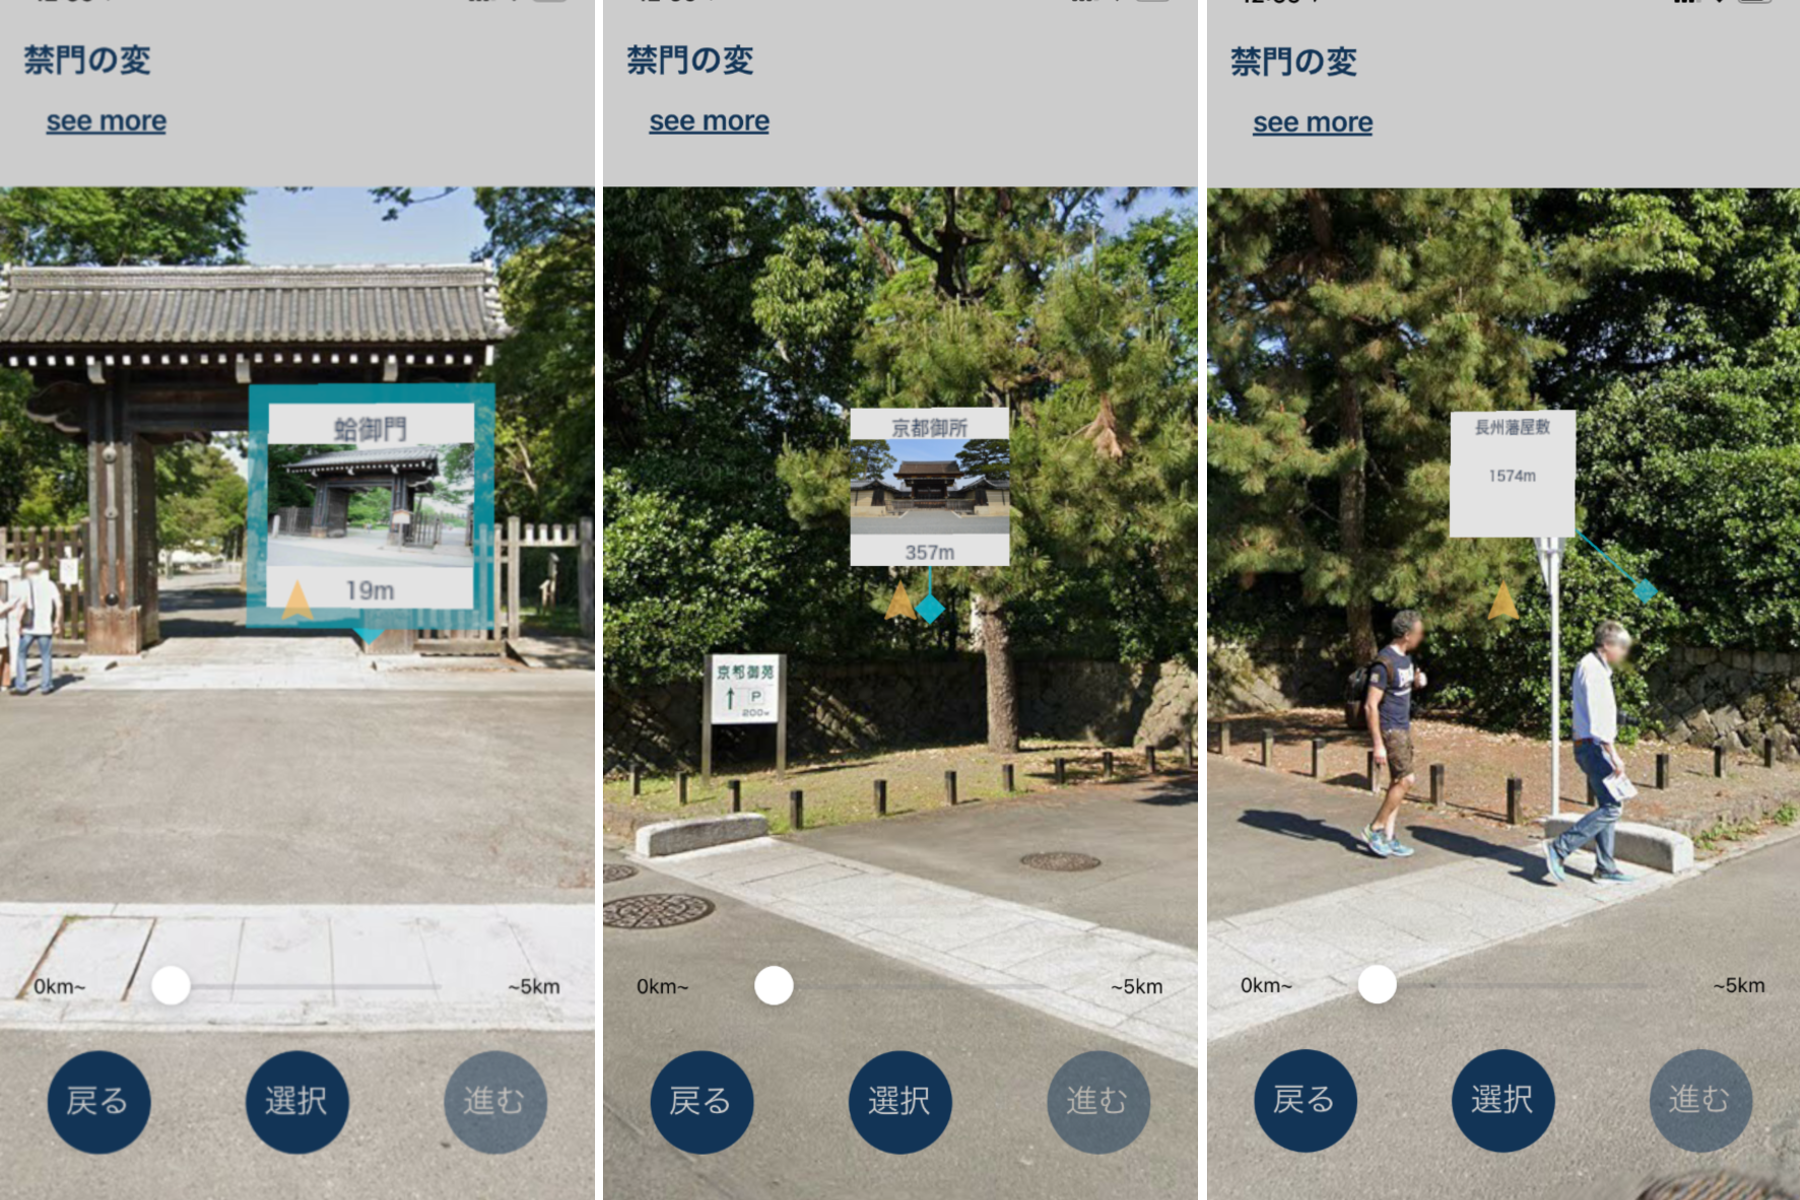
\includegraphics[width=120mm]{images/ar_kinmon.png}
  \caption{「禁門の変」を選択した際の様子} \label{fig:ar_kinmon}
\end{figure}

\begin{figure}[H]
  \centering
  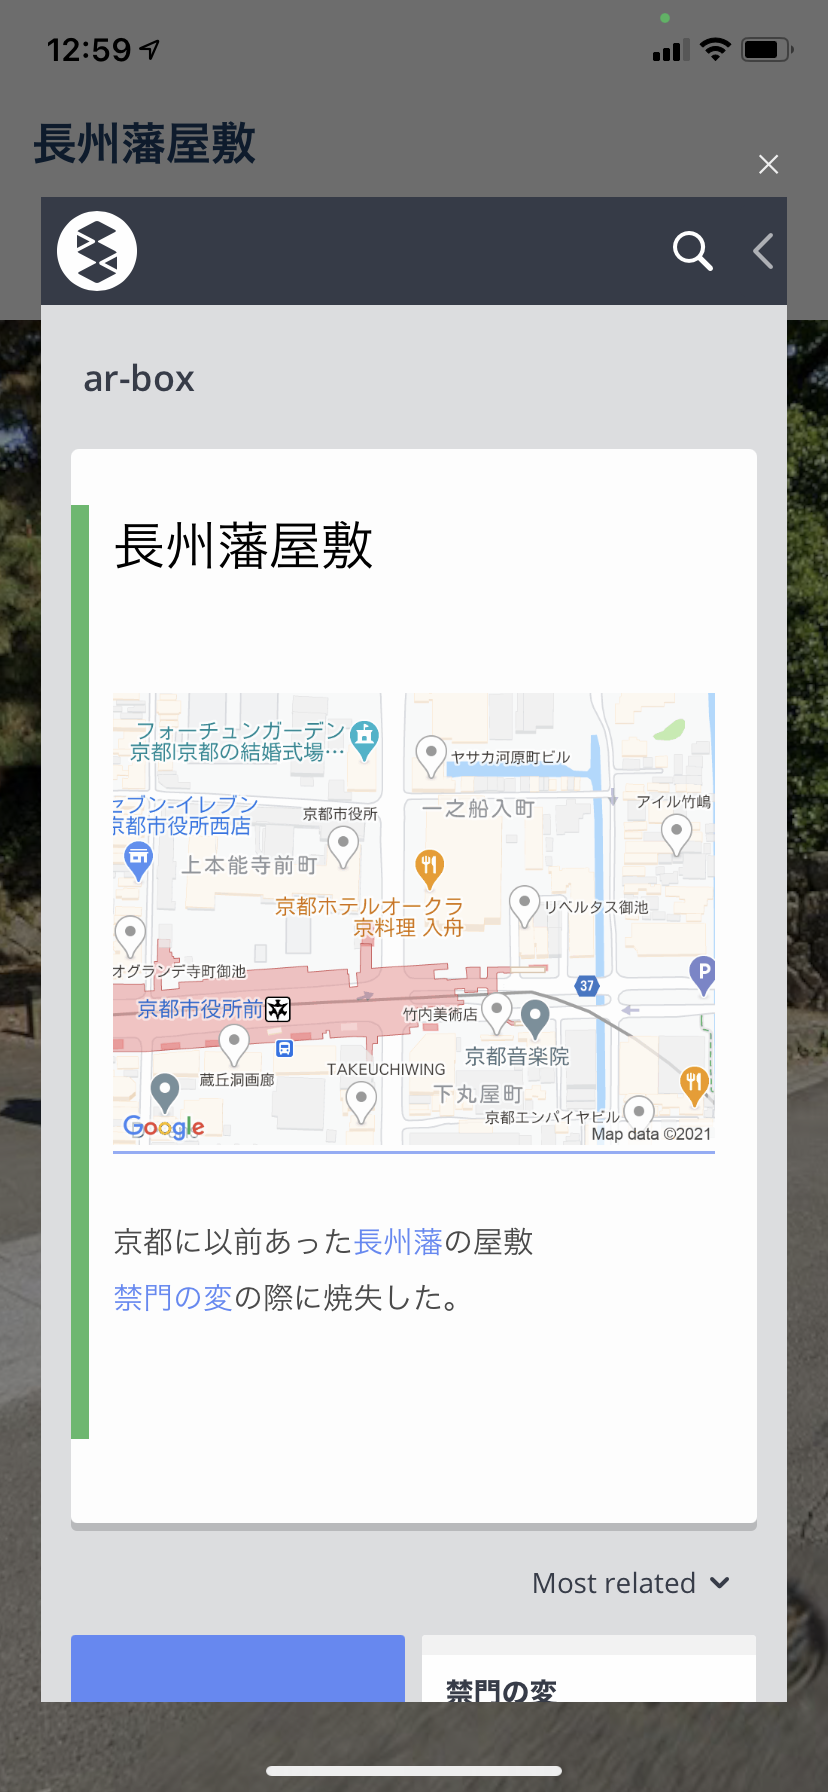
\includegraphics[height=100mm]{images/ar_yashiki.png}
  \caption{詳細説明を見る様子} \label{fig:ar_yashiki}
\end{figure}

\subsection{リンクを利用した柔軟な参照}
\label{link_enum_notation}
本システムでは位置情報を記載したScrapboxページを作成することでAR情報を登録することができるが、それに加えて登録されたAR情報のリンクを利用し新しいページを作ることも可能である。

例えば渋谷からSFCのキャンパスまでの経路を記述したい場合、図のように登録した場所のリンクを列挙すること表現することができる。
Scrapbox上では単にリンクを並べただけだが、HypAR Touchアプリ側では図(TODO:)のように通るべきポイントがARで表示されるようになる。

このように登録された場所をリンクで参照しながらページを作るだけで容易にルート表示や場所のリストを作成することが可能である。
そのため、以下のような用途で活用することができる。

\begin{itemize}
  \item 博物館などでの順路表示
  \item 観光地の行く予定のリスト
  \item 乗り換え案内
\end{itemize}

簡単なリンクによる参照と列挙だけでそれぞれの用途に合ったAR表示を作成できる点は情報の管理にWikiを採用した大きな利点である。


\begin{figure}[H]
  \centering
  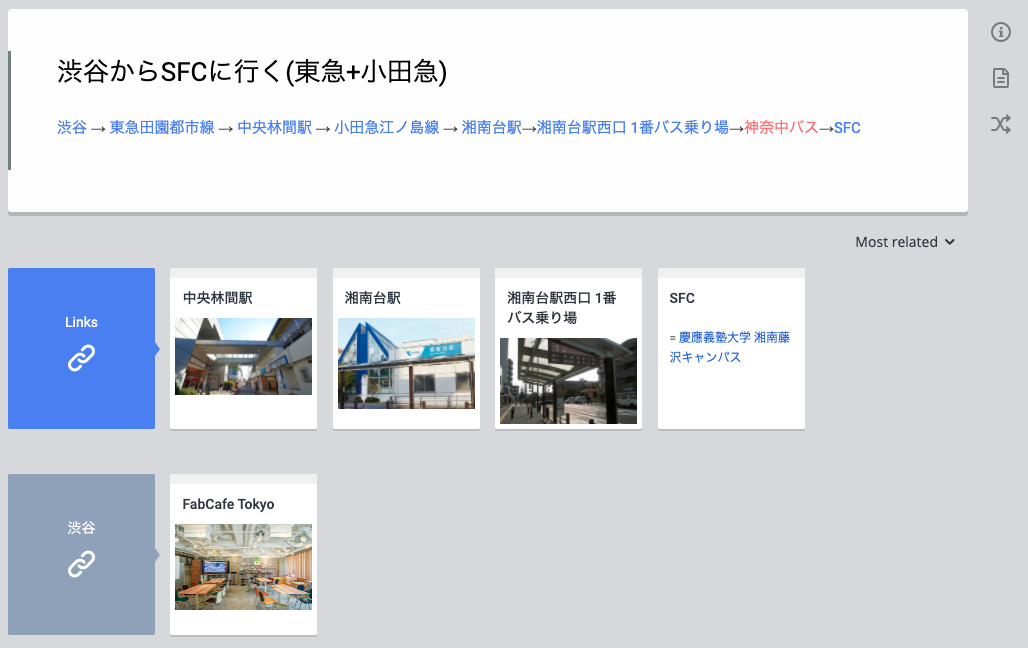
\includegraphics[width=150mm]{images/route_scrapbox.png}
  \caption{リンクを利用したルートの表記例} \label{fig:route_scrapbox}
\end{figure}


\subsection{まとめ}
本章では、本システムによって実現可能な、NFCタグによるインタラクションとリンクによる関連情報の表示機能を活かした利用例について述べた。
タッチというわかりやすいインタラクション、Wikiの持つ拡張性などから、本章で述べた利用例に限らず様々な応用が可能であると考えられる。  % 本文5
\chapter{関連研究}
\label{chap:relatedResearch}

本章では関連研究を紹介し、それらの特徴や本研究との関連性について示す。

\newpage


\section{主要な研究領域}
本研究ではNFCのタッチインタラクション及びwikiベースなARナビゲーションが有用であることを検討した。
本研究に関連する先行研究は大きく以下のように分類できる
\begin{itemize}
  \item ARをナビゲーションに利用する研究
  \item ユーザの位置測位及びコンテキスト情報の取得に関する研究
  \item NFCを用いて情報を取得し、ナビゲーションに応用する研究
  \item AR情報の整理・関連情報推薦にハイパーリンクを利用する研究
\end{itemize}
それぞれについて関連性の高いものを紹介した上で本研究との関連性を示す。

\section{ARをナビゲーションに利用する研究}
ARを地理情報のナビゲーションとして利用する代表的な研究及びシステムを紹介する。

\subsection{A Touring Machine}
Feinerらが開発したA Touring Machine\cite{629922}はヘッドマウント・ディスプレイとスタライスで操作可能な2Dディスプレイで大学のキャンパスの情報を表示するアプリケーションであり、ARを利用した地理情報ナビゲーションの初期研究として挙げられる。
このシステムではGPSによる位置情報と磁気センサによる向きの情報からユーザの位置と向きを推定し、ヘッドマウント・ディスプレイに大学の情報が表示される(図\ref{fig:a_touring_machine_ar})。
また手持ちのスタライスで操作可能な2Dディスプレイが専用のHTTPサーバにつながっており、表示したい情報のリンクに触れるなどの操作をすることでヘッドマウント・ディスプレイでの表示情報が変化する。
ナビゲーションでの表示やシステム構成などが現在のARナビゲーションアプリに通ずる一方で、GPSと磁気センサによる位置測位には精度の面で課題があった。
また当時の技術ではヘッドマウント・ディスプレイとコンピュータを小型化することが難しかったため、図\ref{fig:a_touring_machine_pc}のように装備が大きく、屋外で常用することは現実的でなかった。

\begin{figure}[h]
  \begin{minipage}{0.5\hsize}
    \centering 
    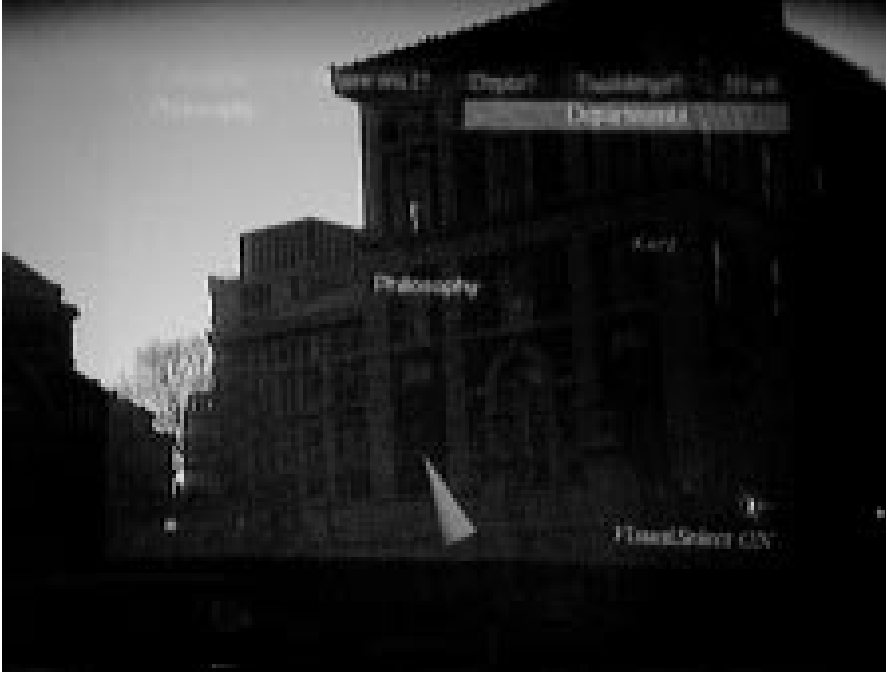
\includegraphics[height=60mm]{images/a_touring_machine_ar.png}
    \caption{表示されたキャンパスの情報} \label{fig:a_touring_machine_ar}
  \end{minipage}
  \begin{minipage}{0.5\hsize}
    \centering 
    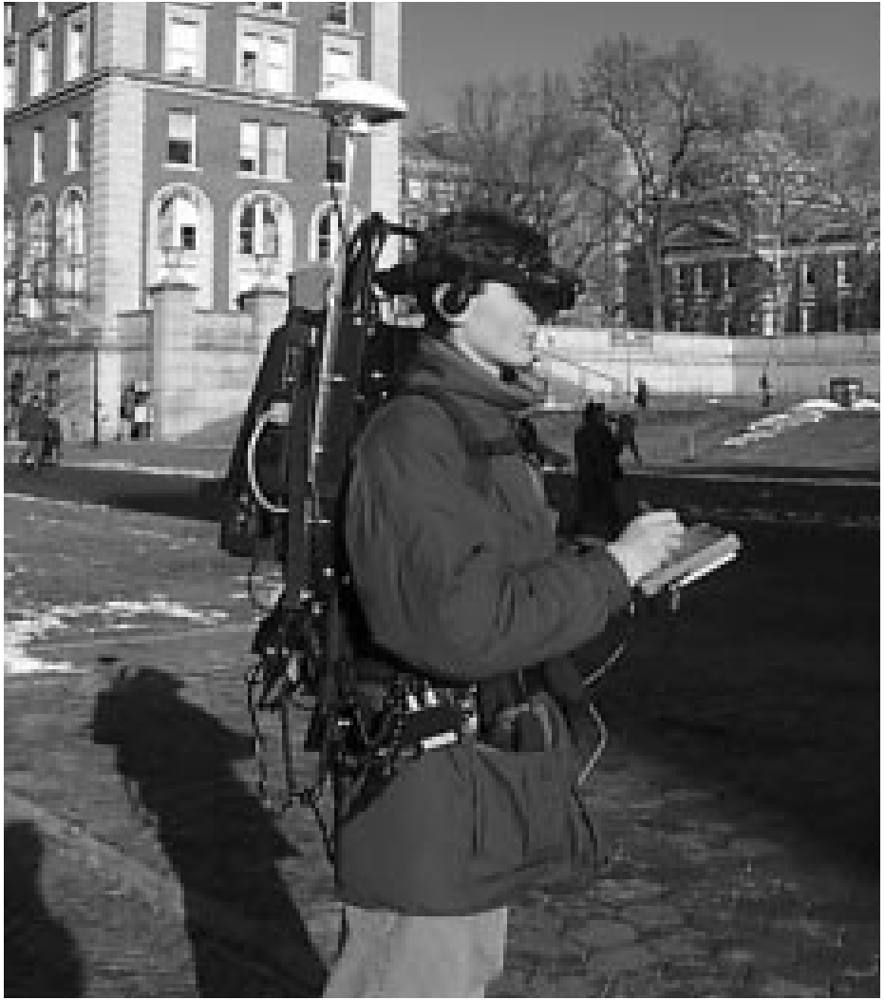
\includegraphics[height=60mm]{images/a_touring_machine_pc.png}
    \caption{実際の装備} \label{fig:a_touring_machine_pc}
  \end{minipage}
\end{figure}


\subsection{KARMA}
FeinerらがKnowledge-based augmented reality\cite{10.1145/159544.159587}で提案したKARMAはレーザープリンターのメンテナンスをARで説明するプロトタイプシステムである。
図\ref{fig:karma}のようにヘッドマウント・ディスプレイによってレーザープリンターの内部機構に関する情報を提示し、ユーザがメンテナンスするときの理解を助けるシステムである。
位置測位には超音波センサを利用しており、正確な位置測位と情報の投影が可能である。
一方で高価で大型な超音波センサをすべての対象に取り付ける必要があり、現実的に利用するにはより良い測位システムを利用する必要があった。

\begin{figure}[h]
  \centering
  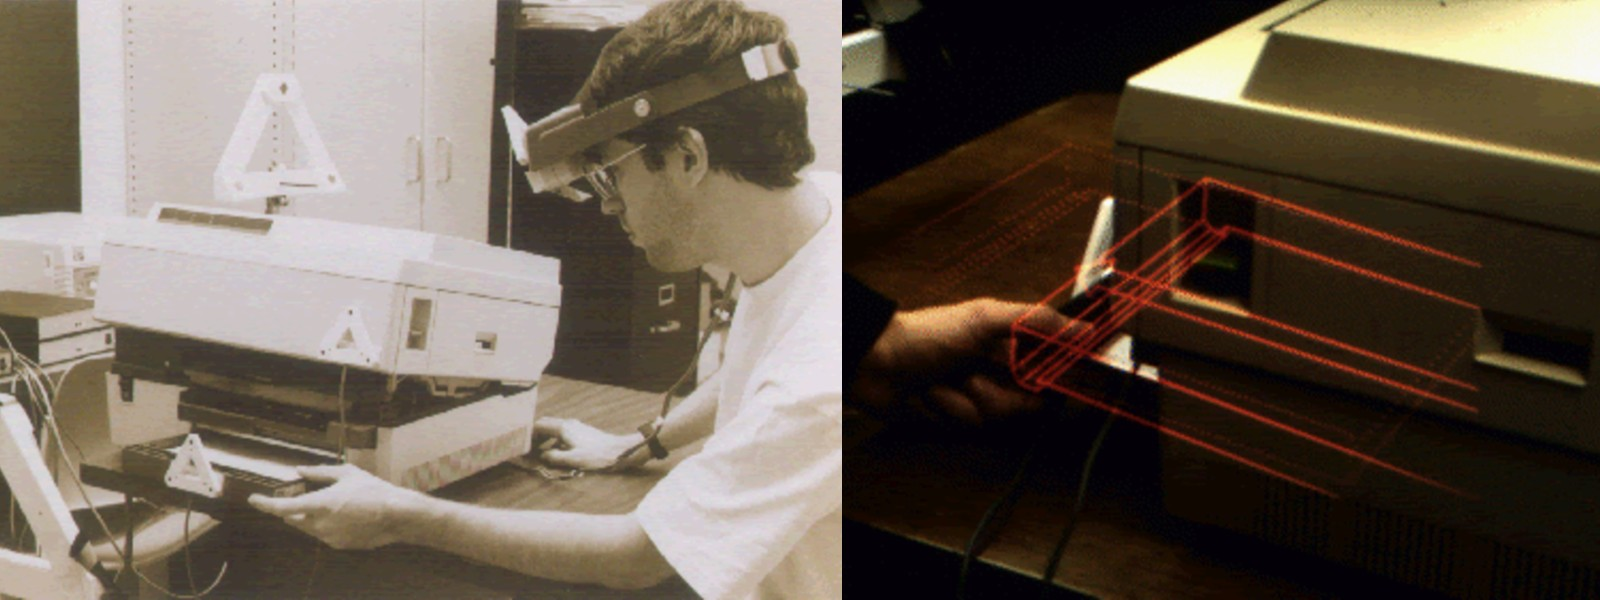
\includegraphics[width=150mm]{images/karma.jpg}
  \caption{KARMA} \label{fig:karma}
\end{figure}


\subsection{MARS}
HöllererらによるMARS\cite{MARS}は上記の「A Touring Machine」及び「KARMA」の方式を組み合わせ、屋外でのARナビゲーションと室内でのARによる地図操作を結びつけたシステムである。
ユーザは屋外でこのシステムを利用することでヘッドマウントディスプレイを通して建物に重ねて表示されたナビゲーションを見ることができる(図\ref{fig:mars_ar})。またPC上で作成された経路情報を実際の景色に投影することも可能である(図\ref{fig:mars_route})。
一方で屋内ではMARSを利用することで、机の平面上に仮想の地図が投影される。この仮想地図はトラックボールや位置センサの搭載されたオブジェクトを利用することで操作でき、屋外のユーザが見ている経路情報などを編集することができる(図\ref{fig:mars_ar_indoor})。
このように屋外でのナビゲーションを編集する環境として屋内でのAR環境を利用し、屋内と屋外のARビューに相互作用をもたせる方式はユーザのAR情報編集の体験向上に大きく寄与すると思われる。
このような編集環境の状態がインタラクティブにARでの情報に作用するという点は本研究とも関連があると言える。

\begin{figure}[h]
  \begin{minipage}{0.5\hsize}
    \centering 
    \includegraphics[height=60mm]{images/mars_ar.png}
    \caption{ARでの表示} \label{fig:mars_ar}
  \end{minipage}
  \begin{minipage}{0.5\hsize}
    \centering 
    \includegraphics[height=60mm]{images/mars_route.png}
    \caption{経路の投影} \label{fig:mars_route}
  \end{minipage}
\end{figure}


\begin{figure}[h]
  \centering
  \includegraphics[height=60mm]{images/mars_ar_indoor.png}
  \caption{屋内での利用} \label{fig:mars_ar_indoor}
\end{figure}

\subsection{NaviCam}
暦本らによるNaviCam\cite{10.1145/215585.215639}はマーカーをカメラで認識し、マーカー応じてその場に即した説明を手持ちの2Dディスプレイやヘッドマウントディスプレイに提示するシステムである。
現在主流になっているマーカーベースのARの初期研究であり、青と赤の線で構成されたカラーコードと呼ばれるバーコードを認識することで状況と対象物の位置を把握し、情報を提示している。
カラーコードの画像認識からARを表示するこの方式は前述のような超音波センサを利用する方式などと比べ圧倒的に低コストであり、カラーコード上での表示は正確であるため屋内での位置測位に有利であると言える。
またコードのパターンによりコンテキスト情報を埋め込むことが可能である点も既存の測位システムにない特徴であった。

\begin{figure}[h]
  \centering
  \includegraphics[height=70mm]{images/NaviCam.png}
  \caption{NaviCam} \label{fig:NaviCam}
\end{figure}


\subsection{Feature-Based Indoor Navigation Using Augmented Reality}
KasprzakらはFeature-Based Indoor Navigation Using Augmented Reality\cite{6597797}で室内での利用を想定したモバイル端末のARナビゲーションのプロトタイプを作成し評価している。
このプロトタイプは画像として登録された特徴的なアイコンなどを元に画像認識(図\ref{fig:FBINUAR_image})から位置情報と向きを推定し、ユーザの目的地を矢印で表示する(図\ref{fig:FBINUAR_ar})ものである。
またこのプロトタイプを利用し、実際に建物内での案内に利用するテストを行っている。
その結果2Dの地図と比べて目的地までの到達時間が短縮され、被験者が立ち止まったり間違えた方向に進む回数も減少したと報告している。
室内での利用を視野に入れている点はGPSなどを利用するシステムと違い、本研究に近いが登録した画像による位置推定には以下のような課題もある。
\begin{itemize}
  \item 特徴的なロゴやアイコンの無いところでは登録できる画像がなく精度が保証できない
  \item 各場所で個別に画像の登録が必要
  \item 距離や明るさなどによっては認識できない可能性がある
\end{itemize}
またこのプロトタイプシステムでは事前に選択した目的地に正確に早く到着することに主眼を置いており、本システムのようにハイパーリンクによる関連情報から周辺譲歩を探索する用途を考えていない点も本研究との違いである。

\begin{figure}[h]
  \centering 
  \includegraphics[height=70mm]{images/FBINUAR_image.png}
  \caption{特徴量による画像認識} \label{fig:FBINUAR_image}
\end{figure}
\begin{figure}[h]
  \centering 
  \includegraphics[height=70mm]{images/FBINUAR_ar.png}
  \caption{矢印による案内} \label{fig:FBINUAR_ar}
\end{figure}


\subsection{Wikitude}
Wikitude(図\ref{fig:Wikitude})は、Wikitude GmbH\footnote{\textsf{TODO:todo}}が開発したモバイル向けARソフトウェアである。
モバイル端末のGPSと磁気センサ、加速度計からユーザの位置と向きを推測し周囲情報をディスプレイに表示する。
コンテンツの追加にはKMLやARML(Augmented Reality Markup Language)と呼ばれるXML互換のフォーマットが使われている。
KMLはGoogleMapなどが対応した地理空間情報の情報記述を目的としたXML互換のファイル形式であり、ARMLはKMLを更に拡張したファイル形式である。
KMLファイルはGoogleMapでの読み込みや作成が可能でありユーザはGoogleMapからAR情報を作成できる。
一方でGPSと磁気センサによる位置推定には精度の面で課題があるだけでなく、GPSの利用できない屋内などでは利用できない欠点がある。
またARでの情報登録する際にGoogleMapなどの地図アプリケーションから作成するかKMLファイルを自身で編集する必要があり、本システムとは以下のような点で異なっている。
\begin{itemize}
  \item 共同編集が難しい
  \item 編集環境がWYSIWYGでない
  \item AR情報同士のハイパーリンクを記述するのが難しい
\end{itemize}

\begin{figure}[h]
  \centering 
  \includegraphics[width=120mm]{images/Wikitude.png}
  \caption{Wikitude} \label{fig:Wikitude}
\end{figure}



\section{ユーザの位置測位及びコンテキスト情報の取得に関する研究}
前節でも挙げたとおりARによるナビゲーションではユーザ位置測位やコンテキスト情報取得には様々な方式が検討されている。
前節に挙げたARナビゲーションシステムでは検討されなかった位置測位システム及びそれらを比較する研究を紹介する。
さらにこれらの測位を複合的に扱いコンテキスト把握につなげるシステムも紹介する。

\subsection{RSSI based Bluetooth low energy indoor positioning}
JianyongらによるRSSI based Bluetooth low energy indoor positioning\cite{7275525}ではBluetooth Low Energy\footnote{\textsf{TODO:todo}}による位置測位が提案されている。
複数の送信機から送られたBluetoothの電波のRSSI(Received Signal Strength Indicator:受信信号強度)を元に位置測位を行うものである。
Bluetoothは現在普及しているモバイル端末のほぼ全てが対応する通信形式であり、Bluetooth Low Energyは使用電力も少なくて済むという利点がある。
一方で複雑な形状の空間や遮蔽物がある場所では測位が難しいという難点があり、正確な測位のためには多くのサンプリングが必要になる。
またGPSやNFCタグなどと比べると一定範囲ごとにBluetoothの送信機が必要になりコストも高いというデメリットがある。


\subsection{Recent Advances in Wireless Indoor Localization Techniques and System}
FaridらによるRecent Advances in Wireless Indoor Localization Techniques and System\cite{Farid2013}では屋内でのユーザの位置測位手法の分析が行われている(図\ref{fig:IndoorLocalization})。
この研究では多くの方式について比較を行っているが、モバイル端末自体以外に特殊な装置を必要としないことを条件にするとGPS、Wifi、Bluetoothの3つに絞られる。
それぞれに対して位置測位の面で以下のような特徴があるとしている。
\begin{itemize} 
  \item GPS\\
    屋外では利用できるが屋内では利用できず、精度も6~10mと良いとは言えない。また位置の取得までに多少の時間がかかるという難点があるとしている。
  \item Wifi\\
    屋内屋外を問わず問わず1~5mの精度で測位できるが、消費電力が高く設置コストが高いという難点がある。
  \item Bluetooth\\
    カバーする範囲が狭く屋内での利用に限られるが消費電力が少なく、2~5mの精度で測位ができる。一方で設備コストが高いことが難点である。
\end{itemize}
このようにモバイル端末で位置測位を行う方式は複数あるが、どれも精度やコストの面で難点がある。
一方本研究で提案したNFCタグによる位置測位はユーザがNFCタグにタッチしなくてはならない点を除くと低コストで正確な位置測位が可能である。
位置測位以外にもNFCタグにコンテキスト情報の結びつけが行える点やタグにタッチするだけでアプリの起動を行えることを踏まえれば十分に有用であると言える。

\begin{figure}[h]
  \centering 
  \includegraphics[width=120mm]{images/IndoorLocalization.png}
  \caption{屋内での位置測位手法の比較} \label{fig:IndoorLocalization}
\end{figure}


\subsection{App Clips}
App Clips\footnote{\textsf{https://developer.apple.com/documentation/app\_clips}}はApple\footnote{\textsf{TODO:todo}}が2020年にiOS向けに発表した機能である。
App ClipsはNFCタグやQRコードの読み込みや位置情報をトリガにして決済、情報提示等を行う仕組みである。
専用のNFCタグやQRコードを読み込んだり、GPSからの情報で特定の位置にいたりすると登録された小規模アプリケーションがインストールなしに利用できる(図\ref{fig:appClips})。
これは上記のようなユーザの位置測位システムを統合しコンテキスト把握に活かしているシステムと言える。
またNFCタグやQRの読み込みからアプリケーションの起動を行う点は本システムと同様である。

\begin{figure}[h]
  \centering 
  \includegraphics[height=90mm]{images/appClips.png}
  \caption{App Clips} \label{fig:appClips}
\end{figure}

\section{NFCを用いて情報を取得し、ナビゲーションに応用する研究}
NFC技術を自己位置推定やコンテキスト情報取得などに利用し、ナビゲーションに役立てている研究を紹介する。

\subsection{Bridging physical and virtual worlds with electronic tags}
WantらはBridging physical and virtual worlds with electronic tags\cite{10.1145/302979.303111}でRFIDを利用し実世界とコンピュータ世界の情報を結びつけるシステムを提案している。
このシステムでは実世界の文書や図書、カードなどにRFIDタグを設置し、これらを専用のリーダーで読み込むことで、関連した情報やURLを推薦したり他のオブジェクトとの関連を示す事ができるようになっている。

ARでの表示は行っていないが、本研究同様にNFCタグをとリーダーを利用してコンテキスト情報を取得しそれに合わせた内容を推薦するシステムである。
この研究からもNFCタグの利用はコンテキスト情報の埋め込みに置いて様々な利用が可能である事がわかる。


\subsection{GoldFish}
増井らによるGoldFish\cite{10.1145/2407696.2407699}はNFCリーダーを搭載したAndroid端末で「実世界GUI」を開発するためのJavaScriptフレームワークである。
Android端末に搭載されたNFCリーダーと加速度センサを用いて実世界に設置されたNFCタグを読み込むことで任意のプログラムを実行できるようになっている。
実行するプログラムはweb上で作成しそのURLをGoldFishに登録するため、ユーザは機能ごとにアプリをインストールする必要ないため汎用性が非常に高い。

GoldFishも本研究同様にNFCタグを実世界のコンテキストの取得に利用している研究である。
またweb上にプログラムを配置し汎用性を高めるという手法は、本研究がARのコンテツをすべてweb上にwikiのプロジェクトとして管理し、ナビゲーションのコンテキストをアプリ側で規定しない点と発想を同じくするものである。

\subsection{Development of an Indoor Navigation System Using NFC Technology}
OzdenizciらはDevelopment of an Indoor Navigation System Using NFC Technology\cite{5954491}でNFCタグを利用した室内ナビゲーションのプロトタイプ「NFC Internal」を作成している。
このプロトタイプはNFCタグにタッチすることでユーザの現在地や向きを把握し、その情報と事前に導入した地図情報から2Dマップでの経路を提示するシステムである。(図\ref{fig:NFC_Internal})

本研究同様、施設内の各所に位置情報の書かれた近距離通信のNFCタグを設置し、タグにタッチされるたびにユーザの場所と向きを更新している。
また屋内での位置測位に近距離通信のNFCタグを利用することの利点としてコストが少ない点、正確な位置と向きの情報が得られる点、通信の応答時間が短い点などを挙げており、これらは本研究が主張するNFCタグの採用理由の一部と一致する。
一方でユーザへの情報提示が2Dの地図とテキストベースであることと、何度もタグにタッチすることで目的地へ最短でたどり着くことに主眼をおいている点が本研究大きく異なると言える。

\begin{figure}[h]
  \centering 
  \includegraphics[width=150mm]{images/NFC_Internal.png}
  \caption{NFC Internalのイメージ} \label{fig:NFC_Internal}
\end{figure}



\section{AR・VR情報の整理・関連情報推薦にハイパーリンクを利用する研究}
ARやVRでの情報を整理するためにハイパーリンクを利用すた研究やプロジェクトを紹介する。
またハイパーリンク情報によってARとVRをシームレスに統合したシステムについても紹介する。



\subsection{VAnnotatoR}
Mehlerらが提案したVAnnotatoR\cite{10.1145/3209542.3209572}はVR/ARでのテキストや画像などのメディアをハイパーリンクを用いて管理し可視化するフレームワークである。
図\ref{fig:VAnnotatoR}のように文書や画像の他に3Dモデルや位置情報同士を関連付け、3Dでそのつながりを可視化する。
さらにユーザの入力によって表示を変えたり関連付けられた場所ワープするような探索機能を備える。

VannotatoRはホロコーストに関連する資料を整理し、可視化することで歴史を解説するStolperwegeプロジェクトが発端となっている。そのため様々な形式の資料と位置情報を互いに関連づけた上でわかりやすく可視化・ナビゲートすることに主眼をおいている。
よってハイパーリンクを利用してARで表示する情報を管理し、それら利用して関連情報を提示するという点で本研究と設計が近いが以下の点で異なっている。
\begin{itemize} 
  \item ハイパーリンク情報の編集環境に関してwikiのような誰でも入力可能なシステムを導入していない
  \item ARの表示における位置推定は考慮に入れていない
  \item HypAR Touchでは文字情報でのみハイパーリンクを形成する
\end{itemize}

\begin{figure}[h]
  \centering 
  \includegraphics[height=90mm]{images/VAnnotatoR.png}
  \caption{VAnnotatoRでのAR表示} \label{fig:VAnnotatoR}
\end{figure}

\subsection{HyperReal}
RomeroらによるHyperRealは\cite{10.1145/900051.900055}仮想現実並びに複合現実におけるハイパーメディアの設計及びその設計に基づいたプロトタイプである。
単なる文字でのハイパーリンクだけでなく様々なメディアをリンクし、ユーザの遷移記録を保存し再現する機能を有するなど複雑なハイパーメディアの構築を行っている。
またプロトタイプでは博物館の案内アプリケーションを作成しており、ARで大まかな情報提示(図\ref{fig:HyperReal_ar})を行った上で詳細を仮想空間で補足する(図図\ref{fig:HyperReal_vr})ようなインターフェースを備えている。
このアイデアは本研究におけるAR情報付近へのワープ機能と類似が見られる。
一方で本研究のようにARで提示する情報の編集環境などには重点を置いておらず、あくまでも時間などを含めた複雑なハイパーメディアの構築に主眼をおいた研究である。
\begin{figure}[h]
  \centering 
  \includegraphics[height=80mm]{images/HyperReal_ar.png}
  \caption{HyperRealでのAR表示} \label{fig:HyperReal_ar}
\end{figure}

\begin{figure}[h]
  \centering 
  \includegraphics[height=80mm]{images/HyperReal_vr.png}
  \caption{HyperRealでのVR表示} \label{fig:HyperReal_vr}
\end{figure}


\subsection{Annotation authoring in collaborative 3D virtual environments}
小林らによるAnnotation authoring in collaborative 3D virtual environments\cite{10.1145/1152399.1152452}では、Kayらが主導した仮想OSプロジェクトCroquet\cite{10.5555/1009376.1009395}でを拡張したアノテーションシステムを提案している。
具体的には以下のような機能をもつ注釈システムを提案している。
\begin{itemize} 
  \item 特定のシーン内に注釈をつけそれらをあらゆるシーンからシーンから参照できるようにする
  \item 追加された注釈をオブジェクトとして空間上に配置しまとめることができる
  \item 注釈をフィルタするためのシステム「Interactor」を作成
  \item 注釈の変化を可視化する
\end{itemize}
これらの機能のうち、追加された注釈をオブジェクトとして空間上に配置しまとめることができる点は第\ref{link_enum_notatio}節の「リンクを利用した柔軟な記法」と類似が見られる。
表示するもののフィルタに関しても本研究での課題と言える。
一方で本研究ではAR/VRで表示する情報とその他のwikiページを等価に扱ったリンク構造を採用しており。この研究とは大きく異なると言える。

\subsection{MagicBook}
BillinghurstらによるMagicBook\cite{10.1145/634067.634087}ははARとVRの間のシームレスな移行を可能にするシステムのプロトタイプである。
Magicbookでは実際の本を利用し、本にマーカーを埋め込むことでヘッドマウントディスプレイからの自由な視点を持ったARを提供する。
さらにARで表示された状態でハンドルのスイッチを押すとシームレスにVRに移行し、自由に仮想空間状を移動することが可能になる(図\ref{fig:MagicBook})。
MagicBookのARのビューからVRへとシームレスに切り替えることでより詳細な情報を表示するという考えは本システムの移動機能に類似点が見られる。
一方で、本研究での移動はあくまでも場所から場所への移動による探索を主眼としているに対し、MagicBookは1つのAR情報を更に細くする形でVRを展開しているという点で用途に異なりがあるといえる。


\begin{figure}[h]
  \centering 
  \includegraphics[width=120mm]{images/MagicBook.png}
  \caption{MagicBookでのAR(左)とVR(右)} \label{fig:MagicBook}
\end{figure}


  % 本文6
\chapter{考察}
\label{chap:consideration}

本章ではHypAR Touchの利用者の意見や自身の運用経験をまとめ、諸問題や新しい可能性について述べる。

\newpage


\section{評価}
本システムのうち、NFCタグによるインタラクション部分のプロトタイプとなる「TouchAR」は2019年後半から後半から開発を行っており、ORF2019\footnote{ \textsf{https://orf.sfc.keio.ac.jp/2019/} }にてDrawWikiの展示発表を行った。
またその後も2020年11月からの2ヶ月に渡り使用した様子を共有したり、実際にユーザに使ってもらうことで意見を集めた。
本節ではユーザからのフィードバックおよびTouchARの展示発表で得られた感想、筆者の運用経験をまとめる。

\subsection{意見・感想}

第\ref{problems}節で述べたARによるナビゲーションの問題点や、その解決策としてNFC技術とwikiにより情報を管理する本システムについて多くの同意が得られた他、以下のような感想や意見が寄せられた。

\paragraph*{Wikiを採用したことによる編集の容易さ}
既存のAR表示システムでは情報の追加のフォーマットが決まっている事が多く、一般ユーザが自発的に情報を追加編集することが難しい。
一方本システムではScrapboxページを作り、googleMapのURLを貼り付けるだけでARの情報を追加できるため、AR情報の追加という感覚なしに気軽に情報を追加できるという意見があった。
また既存のScrapboxのプロジェクトのうち地図情報があるものがそのままARで表示できる拡張性も評価された。

\paragraph*{NFCタッチによる起動}
既存のARナビゲーションシステムとして

\subsection{筆者の運用経験}
キャンパスでの利用を想定したフィールドワークを行った。
また自身の訪れたことのない場所の探索フィールドワークを複数回行った。

\paragraph*{リンクに基づく優れた参照性}
Scrapboxにはフォルダやタグ・ラベル等のメモやイラストを分類し管理するための機能は存在しない。
全てのAR情報がフラットに置かれているが、リンク情報に基づいて関連する情報が表示されるため



\subsection{問題点・要望}
以下のような問題点が明らかになった。
\begin{enumerate}
  \item 二次リンクについて\\
  一次的なリンクだけだと直接関連のあるものしか見れないので二次リンクまで見えるとよいのではないかという意見が挙げられた。
  Scrapboxのように二次リンクを表示することでより探索感は上がるとは考えるが、その分画面で表示する情報が急激に増えるため工夫が必要になる
  \item 登録情報が増えた場合の対処\\
  誰もが情報を追加できるという利点があるが、一方で登録された情報が増えてカオスになるというデメリットがあるという意見が挙げられた。
  現在は距離によってフィルターを行っており、画面下部のスライダーで調整ができるがそれでも表示する件数が多くなるとユーザが欲しい情報を見つけるための障壁になる。
\end{enumerate}


\section{考察}

\subsection{設計の妥当性}
本システムは既存のものとは異なる新しい位置測位システムと情報管理を採用しているが実際に利用したりデモを体験したユーザからは概ね好意的に受け入れられ、NFCタグを利用したインタラクションとwikiを利用した情報管理をARに組み合わせた本システムの設計指針は正しかったといえる。
また本研究で述べたARナビゲーションに対する問題意識にも多くの共感を得られたことから、本システムをベースにして様々な改善や拡張を行うことで、より良いARナビゲーションアプリを生み出せると考えられる。

\subsection{解決すべき課題}

\begin{enumerate}
  \item 一次リンクだけでは関連情報が見つけにくい\\
  一次リンクだけを表示すると単語で直接的に関係のあるものしか見れないため二次リンクを積極的に活用していくべきであると考える。
  一方で単純に二次リンクをすべて表示することは画面の制約などから難しいためフィルターか、推薦機構が必要である。
  一例としてリンクを分析した上で接続の多いノードを大きく提示したり推薦する方法が考えられる。
  \item 登録情報が増えたときに情報が見にくくなる\\
  現在はユーザのいる場所からの距離によるフィルターを行っているが、情報量が地域によって違うことが想定されるためこの手法が最適とは限らない
  この問題に対しては対しては以下のような工夫が可能であると考える。
  \begin{itemize}
    \item 距離順や接続ノードの数などでソートし上位のみを表示する。
    \item タグ自体にフィルター用の変数を登録することでタッチしたときからデフォルトでフィルターがかかるようにする。
    \item ユーザの個人情報から関心度の高そうなものを優先的に表示する。
  \end{itemize}
   
\end{enumerate}

\subsection{問題点の検証}
本システムにおいて第\ref{problems}節で述べた問題点が克服されているかどうかを問題点毎に検証する。
\begin{itemize}
  \item 立ち上げるまでのインタラクションが面倒 \\
  NFCタグを利用することでタッチするだけでアプリを起動することができる。
  \item 位置測位の方法によって精度や用途が大きく限られる \\
  屋内/室外を問わずナビゲーションに十分な精度でARを表示できる
  \item 情報の登録・編集が面倒 \\
  wikiを利用し、ページとARで表示する情報を対応させることで誰もが容易に登録・編集可能である。
  \item 関連情報を参照・管理することができていない \\
  ハイパーリンクを利用することで関連情報を参照・管理できる
  \item 汎用性のあるアプリケーションがない \\
  環境に左右されない位置測位とジャンルを問わずリンク参照から管理できる汎用性を持っていると言える。
\end{itemize}
以上のように、第\ref{problems}節で述べたすべての点に関して問題が解決していることがわかる。  % 本文7
\chapter{結論}
\label{chap:conclusion}

本章では本研究を総括する。

\newpage



\section{研究の成果}
本研究では、NFCを利用したインタラクションとAR情報をWikiで管理するシステムを組み合わせた次世代のARナビゲーションシステム「HypAR Wiki」の提案を行った。

まず第\ref{chap:background}章において、ARによるナビゲーションの問題点を2次元上での既存メディアの進化と比較しながら分析した。ARでナビゲーションを行う既存システムの現状をとりあげ、ARナビゲーションシステムの問題点が根本的に解決されていないことを示した。

第\ref{chap:design}章では、第\ref{chap:background}章で述べたARナビゲーションシステムの問題点に対する有効的な解決方法を提案した。また、それに基づき本研究で開発した次世代ARナビゲーションシステム「HypAR Touch」の基本構成と使い方について述べた。

第\ref{chap:implementation}章では、「HypAR Touch」のアプリケーション構成と詳細な実装について述べた。

第\ref{chap:usage}章では、「HypAR Touch」によって実現可能な応用例について述べた。

第\ref{chap:relatedResearch}章では、本研究に関連する研究を紹介し、それぞれのアプローチの特徴と問題点を分析した。

第\ref{chap:consideration}章では、筆者による運用経験やユーザからのフィードバックをもとに本研究の有効性と問題点を分析した。

\section{総括}
本研究ではNFCタグに触れるというインタラクションからARナビゲーションを表示でき、表示するAR情報の管理をWikiで行える「HypAR Touch」の開発を行った。
HypAR TouchはNFCタグに触れるインタラクションとWiki等の技術の組み合わせによって、ユーザの位置推定の問題やAR情報の編集・参照が難しいといった問題を解決した。。
また有用な活用例を示し、既存のシステムより優れた点があることを示した。
今後は第\ref{chap:consideration}章で述べた問題点についての改善や、システム改善を行っていく。  % 本文8

\begin{acknowledgment}

  慶應義塾大学環境情報学部 増井俊之教授には学部から4年半の長きに渡りご指導を賜りました。深く感謝いたします。また、本研究の副査としてご意見、ご助言を頂きました中西泰人教授、武田圭史教授に感謝いたします。
  また自身の研究について幅広い議論をしていただいた政策・メディア研究科博士課程の田中優氏、大和比呂志氏を初め、様々な形でアドバイスをくださった増井俊之研究会所属の学生及びOB諸氏に感謝いたします。
  \\
  \begin{flushright}
      2021年1月 慶應義塾大学 政策・メディア研究科 修士2年 左治木隆成
  \end{flushright}
  
  \end{acknowledgment}  % 謝辞。要独自コマンド、include先参照のこと

\begin{bib}[100]
% BibTeXを使う場合
\bibliography{main}

%\begin{thebibliography}{#1}
%
%  \bibitem{参照用名称}
%    著者名: 
%    \newblock 文献名,
%    \newblock 書誌情報,出版年.
%
% \bibitem{hoge09}
%   ほげ山太郎,ほげ山次郎:
%   \newblock ほげほげ理論のHCI分野への応用,
%   \newblock ほげほげ学会論文誌,Vol.31,No.3,pp.194-201,2009.
% 
% \bibitem{hoge08}
%   Taro Hogeyama, Jiro Hogeyama:
%   \newblock The Theory of Hoge,
%   \newblock {\it The Proceedings of The Hoge Society}, 2008.
%	
%\end{thebibliography}



\end{bib}

  % 参考文献。要独自コマンド、include先参照のこと
% \appendix
% \include{92_appendix}    % 付録

\end{document}
